

\documentclass[a4paper,12pt]{report}
\usepackage[T1]{fontenc}
\usepackage[utf8]{inputenc}
\usepackage[magyar , english]{babel}

\usepackage{times}
\usepackage[top=2.5cm, bottom=2.5cm, left=3.7cm, right=2.5cm]{geometry}
\linespread{1.0}
%\pagestyle{headings}
% \usepackage{fancyhdr}
% \pagestyle{fancy}
% \addtolength{\headheight}{\baselineskip}
% \renewcommand{\headrulewidth}{1.6pt}
 
\usepackage{amsmath,amssymb,amsfonts,amsthm,amstext}

\usepackage{float}
\usepackage{multicol, multirow}
\usepackage{array}
\usepackage[justification=centering]{caption} %for centering the captions

\usepackage[center]{subfigure} %for subfigures
\subfiglabelskip=0pt

\usepackage{todonotes}
\usepackage{fixltx2e}
\usepackage{xcolor}
% \usepackage{varioref}
\usepackage{hyperref}
\hypersetup{
  colorlinks   = true, %Colours links instead of ugly boxes
  urlcolor     = blue, %Colour for external hyperlinks
  linkcolor    = red, %Colour of internal links
  citecolor   = green %Colour of citations}
}

\usepackage[numbered]{bookmark}
\bookmark[page=1,level=0]{Sample document}
% \hypertarget{tocpage}{}
% \usepackage[nottoc]{tocbibind} % linkelés jav

\usepackage{listings} %codes

\usepackage{graphicx}
\graphicspath{{figures/}}
\usepackage[ final ]{pdfpages}
\includepdfset{ pages=-,  pagecommand={\pagestyle{headings}}}
%\usepackage[section]{placeins}

\usepackage{gensymb}
\usepackage{ulem}

\usepackage{verbatim}
\usepackage[numbered, framed ]{mcode} % autolinebreaks %MatLab code

%\usepackage[maxfloats=100]{morefloats}

% !TEX spellcheck = language_tag

\usepackage{titlesec}


%\usepackage{showkeys}

\title{Időlépéses módszerek összehasonlító elemzése és hibrid módszer alkalmazása}
\author{Balla Réka}
\date{2014}

%\subtitle{Diplomaterv, vázlattervi szeminárium}
%\author{Balla Réka \and \\ Dr. Joó Attila László \and Dr. Németh Róbert}
%\institute{Budapesti Műszaki- és Gazdaságtudományi Egyetem, \\ Hidak és szerkezetek tanszéke}

% konzulensek!!!!!!

\begin{document}

\titleformat{\chapter}[hang]
  {\normalfont\LARGE\bfseries}{\thechapter. }{0em}{} 

  % \renewcommand{\chaptermark}[1]{%
% \markboth{\thechapter.\ #1}{}}
 \thispagestyle{empty}
 \begin{center}


\begin{figure}[t]
\centering
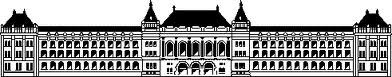
\includegraphics[ width=0.8\textwidth]{bmelogo.png}
\end{figure}
\textbf{\large{Budapesti Műszaki és Gazdaságtudományi Egyetem \\ Építőmérnöki Kar} \\ }
\vspace{3.5cm}

\textbf{\huge {DIPLOMAMUNKA\\}}
\vspace{1 cm}
 \textbf{\Large {Időlépéses módszerek összehasonlító elemzése \\ és hibrid módszer alkalmazása\\}
  \vspace{2cm}														% K\'etsoros c?m eset\'en ?rjuk \'at 4cm-re
  \textbf{\Large{Balla Réka} \\ }}
\vspace{3.5cm}

 \textbf{\large{Konzulensek:\\}} 
 \vspace{0.8 cm}
\begin{tabular}{ccc}  
\textbf{ \large{Dr. Joó Attila László}} & \hspace{1.5 cm} & \textbf{\large{Dr. Németh Róbert}}\\
 \large{egyetemi docens} &   & \large{egyetemi docens}\\
\end{tabular}
 %\normalsize{BME Hidak és Szerkezetek Tanszék} & \normalsize{BME  Tartószerkezetek Mechanikája Tanszék} 
 
 \vspace{3 cm}
\textbf{\Large{2014}}

\end{center}
 
% \maketitle
\newpage

% \pagestyle{headings}
\setcounter{page}{1}
\pagenumbering{roman}
% \pagestyle{empty}

\selectlanguage{magyar}

\begin{abstract}

{\ }

Magyarország, a jelenlegi kutatások szerint, közepes szeizmicitású terület. Korábban kevésbé tartották fontosnak  hazánkban a földrengésre való tervezést, azonban a szeizmikus hatások vizsgálata az Eurocode-8 bevezetésével előtérbe került. A tervezési  igények növekedésével a témára irányuló kutatások  megsokszorozódtak, mivel az új épületek, illetve a már meglévő szerkezetek földrengés elleni védelme új szerkezeti megoldásokat igényel.  

Diplomamunkámban az építőmérnöki szerkezetek  szeizmológiai védelmére irányuló kutatások lehetőségeit mutatom be. Ismertetem a dinamikus számításokhoz alkalmazható numerikus számítási módszereket, valamint egy viszonylag új numerikus számításokkal összekötött kísérleti eljárást,  a hibrid szimulációs módszert.

A szerkezeteket jellemző dinamikus mozgásegyenletek megoldása  a gyakorlatban alkalmazott nagyobb rendszerek esetében analitikusan általában nem lehetséges. A számítógépes kapacitás növekedésével előtérbe kerültek a numerikus időlépéses integráló módszerek, melyekre számos algoritmust fejlesztettek. Dolgozatomban ismertetem elméleti hátterüket, főbb jellemzőiket, és bemutatom a legfontosabb eljárásokat.

Az algoritmusok alapján saját lineáris és nemlineáris megoldó programokat fejlesztek. Bemutatom a lineáris megoldó program használatát gerjesztett rezgések vizsgálatára, valamint szabadrezgés esetében az egyes algoritmusok stabilitásának és pontosságának elemzésére. A nemlineáris megoldó programot alkalmazom statikus probléma vizsgálatára különböző csillapítási tényezők mellet, majd használom dinamikus probléma vizsgálatára is eltérő terhelésekkel, és szemléltetem a nemlinearitás hatását a szerkezet elmozdulásaira. Ezek után elvégzem a programok verifikálását szakirodalmi példákkal.

Dolgozatom második részében  a hibrid szimulációs  eljárást mutatom be. Egy összefoglaló tanulmányban jellemzem az eljárás előnyeit, kivitelezésének lehetőségeit, és a megvalósításának módját. Bemutatom, melyek a szimuláció legfontosabb elemei, és milyen műszerek szükségesek a vizsgálatok elvégzéséhez. 

Egy kiválasztott időlépéses algoritmus alkalmazásával saját hibrid szimulációs programot fejlesztek. A program használatát  bemutatom  egy nemlineáris elemet is tartalmazó szerkezet vizsgálatán keresztül. A feladatban  egy ismert földrengésterhet, az El Centro-t működtetem a szerkezetre, és  leírom a szükséges adatok beolvasásának módját, továbbá elvégzem a hibrid program verifikálását ugyanannak a szerkezetnek a nemlineáris megoldó programban való  számításának eredményeivel. 

Végül bemutatom a hibrid szimulációs eljárás alkalmazását egy képlékeny anyagú szeizmikus szigeteléssel ellátott épület viselkedésének vizsgálatára. Az eredményeket összehasonlítom egy fix megtámasztású épület és egy rugalmas anyagú szeizmikus szigeteléssel ellátott szerkezet  lineáris vizsgálatával kapott eredményekkel. Elvégzem az  eredmények kiértékelését, és ez alapján értékelem a szeizmikus szigetelés szerkezeti viselkedését.





\end{abstract}


\selectlanguage{english}

\begin{abstract}



{\ }

Current research indicates that Hungary is a moderate seismicity area. Earlier in our country earthquake engineering was less important, however, the examination of the seismic effects came to the fore by introducing Eurocode-8. Beside increasing necessity of earthquake engineering, researches relating to the topic have multiplied since  the seismic protection of the new buildings, and existing ones require new structural solutions.

The objective of my thesis is to demonstrate the  opportunities of researching seismic protection of civil engineering structures. Numeric methods used for dynamic calculations is reviewed, and a relatively new method called hybrid simulation  based on connecting numerical calculations with experimental testing is specified as well. 
It is  not generally possible to solve dynamic equation of motion  analytically for larger structures used in practice. Numeric time-stepping methods came to the forefront because of increasing computer capacity. Different integration  algorithms have been developed for structural dynamics. My thesis describes the theoretical background and  the main characteristics of time-stepping process and presents the most relevant integration algorithms.

I developed programs for solving linear and nonlinear problems based on the integration algorithms. I demonstrate how to use the linear solver program to excited vibration tests and to free vibration tests  to examine  the stability and the accuracy of algorithms. The nonlinear solver is used to  test static problem for different damping rates, and it is used to examine a dynamic problem with different loads to show the effect of nonlinearity in displacement  responses. The program is verified by scientific literature examples.

In the second part of my thesis, the hybrid simulation method is presented. The advantages of the process, the options of implementations and the manner of implementation  are summarized in a study. Key components and required instruments  of  simulation  are also introduced.
 
I developed a hybrid simulation program using a selected time-stepping algorithm.  I display  how to use the program through an examination of a  structure containing nonlinear elements. A well-known earthquake load,  namely El Centro, is actuated on the structure and the method of retrieving  necessary data is described. In addition, verification of hybrid program is performed by analysing the same structure with the nonlinear solver program.

Finally  I present the using of  a hybrid simulation method by testing the response of a structure with  base isolation made of ductile material. The results are compared with the results of linear analysis of a fixed-base building and  an isolated building, where base isolation is made of flexible material. Evaluation of the results is performed, and the behaviour of the base isolation is rated according to the results.




\end{abstract}


\selectlanguage{magyar}

\tableofcontents
% \bookmark[dest=tocpage,level=0]{Tartalomjegyzék} 


\listoffigures
% \bookmark[dest=tocpage,level=0]{Ábrák jegyzéke} 



\listoftables
% \bookmark[dest=tocpage,level=0]{Táblázatok jegyzéke} 

\newpage
{~ }\\
\vspace{5cm}

\section*{Köszönetnyilvánítás}
\addcontentsline{toc}{section}{Köszönetnyilvánítás}

Ezúton szeretnék köszönetet mondani tanáromnak, Dr. Németh Róbertnek, hogy a  diplomafélévemben kitartóan ösztönzött, segített, és  munkámat alaposan és kritikusan ellenőrizte. Köszönöm, hogy  tanulmányaim során végig önzetlenül mentorált.

Köszönöm konzulensemnek, Dr. Joó Attilának, hogy felajánlotta ezt az izgalmas témát, lehetőséget biztosított dolgozatom sikeres megírásához, és hasznos szakmai tanácsaival segítette munkámat.

Szeretném megköszönni a családomnak és a barátaimnak diplomamunkám megírásához nyújtott segítségüket, és azt a rengeteg támogatást és bátorítást, amit képzésem ideje alatt kaptam tőlük.

\newpage
\pagestyle{headings}
\setcounter{page}{1}
\pagenumbering{arabic}




\chapter{Bevezetés}                  

{\ }

Magyarországon a földrengés aktivitás a lemezperemi területekhez  képest alacsony, viszont ez koránt sem jelenti azt, hogy elhanyagolható. A jelenlegi kutatások szerint a Kárpát-medence közepes szeizmicitású terület. Az ország területén évente 100-120 alig érezhető, 2,5-nél kisebb magnitúdójú  és  4-5 már jól érezhető, de károkat még nem okozó, 2,5-3 magnitúdójú földrengés fordul elő.  Jelentősebb károkat okozó rengés 15-20 évenként, míg erős, nagyon nagy károkat okozó, 5,5-6 magnitúdójú földrengés 40-50 évenként pattan ki. A legnagyobb ismert, Magyarország területén kipattant  földrengés 1763-ban  Komárom területén keletkezett, 6,3 körüli magnitúdóval. Földrengés szempontjából a legveszélyeztetettebb területek Eger és környéke, Komárom és Mór környéke valamint Jászberény, Kecskemét és Dunaharaszti környéke \cite{mónus,évkönyv}. 

Hazánkban földrengéstervezésre, az Európai Unió tagállamaként,  az Európai Unió egységes földrengésszabványa, az Eurocode-8 (MSZ EN 1998 \cite{ec8}) van érvényben, 2009. január 01. óta. A szabvány célkitűzései az emberélet védelme -a teherbírási követelmények kielégítésével-, az épületek  károsodásának korlátozása -a használhatósági határállapotok kielégítésével-, és a polgári védelem szempontjából létfontosságú épületek (kórház, mentőállomás, telefonközpont, tűzoltósági épület, transzformátorállomás, stb.) működőképességének biztosítása. Nagyon fontos továbbá a földrengésállóság biztosítása veszélyes ipari létesítmények (pl. atomerőmű, kőolaj finomító, gázterminál) esetében  a katasztrófahalmozódás elkerülése érdekében.

A földrengés károsodás kockázatának csökkentése történhet a rezgést csökkentő és elszigetelő szerkezeti rendszerek beépítésével. Ez megvalósítható  aktív vagy passzív kontroll rendszerrel. Aktív kontroll rendszer esetén az épületben dinamikus terhelés hatására számítógép vezérléssel beindul egy lengés-kiegyensúlyozó hidraulikus rendszer, passzív kontroll rendszer  esetében pedig az alapozás és a felmenő szerkezet közé rugalmas-képlékeny energiaelnyelő  szerkezeti rendszer, úgynevezett szeizmikus szigetelés kerül beépítésre. Ezeket a  szerkezeti megoldásokat akár már meglévő épületszerkezeteken is lehet alkalmazni utólagos beépítéssel. 

A kontroll rendszerekre napjainkban egyre több megoldás válik elérhetővé, azonban az így még összetettebbé váló épületszerkezetek viselkedése kevésbé ismert, és nehezen modellezhető. Az ilyen szerkezetek viselkedésének vizsgálata szeizmikus vagy más dinamikus terhelésre  a mai építőmérnök kutatók fontos feladata.%\\[3pt]

A nagyobb szerkezetekre felírt dinamikus mozgásegyenletek megoldása már önmagában is összetett feladat. A többszabadságfokú rendszerek mozgása mátrix - differenciálegyenlettel jellemezhető, melynek megoldására több matematikai metódus is létezik, azonban az analitikus megoldás nem mindig lehetséges a számítógépek kapacitásának véges volta miatt, ezért sokszor a numerikus eljárások kerülnek előtérbe. 

A többszabadságfokú lineáris rendszerek tetszőleges erővel gerjesztett rezgését az alábbi mátrix-differenciálegyenlet írja le:
%
\begin{equation}
\label{rezgegy}
\mathbf{M}\mathbf{\ddot{x}}(t)+\mathbf{C}\mathbf{\dot{x}}(t)+\mathbf{K}\mathbf{x}(t) = \mathbf{p}(t),
\end{equation}
%
ahol $\mathbf{M}$ a  szerkezetre vonatkozó tömegmátrix, $\mathbf{C}$ a csillapítási mátrix, $\mathbf{K}$ a szerkezet merevségi mátrixa, $\mathbf{\ddot{x}}(t)$, $\mathbf{\dot{x}}(t)$ és $\mathbf{x}(t)$ rendre a szerkezet időtől függő gyorsulás-, sebesség- és elmozdulásvektora és $\mathbf{p}(t)$ pedig a tehervektor az idő függvényében.

A nemlineáris rendszerek gerjesztett rezgését pedig a következő differenciálegyenlet jellemzi:
\begin{equation}
\label{rezgegy_nemlin}
\mathbf{M}\mathbf{\ddot{x}}(t)+\mathbf{C}\mathbf{\dot{x}}(t)+f_s(\mathbf{x}) = \mathbf{p}(t),
\end{equation}
%
ahol $f_s(\mathbf{x})$ a szerkezetre vonatkozó, elmozdulástól függő rugalmas visszatérítő erő, a többi pedig rendre megegyezik a \eqref{rezgegy} egyenletnél ismertetett jelölésekkel.

Ezek megoldására adott kezdő időpontbeli elmozdulás- és sebességvektor, azaz $ \mathbf{x}(0) = \mathbf{x}_0$  és $\mathbf{\dot{x}}(0) = \mathbf{v}_0 = \mathbf{\dot{x}}_0$  kezdeti feltételek esetén direkt integrálás alkalmazása elterjedt, mert komplex modálanalízis használata nagyobb rendszerek esetén bonyolult, vagy egyáltalán nem vezet megoldásra. A modálanalízis nagyméretű feladatokra alkalmazásánál kérdés a módusok összegzése és az alkalmazható csillapítási mátrix, a számítás pedig meglehetősen bonyolult.  A kezdő időpontbeli gyorsulások értéke, azaz az $\mathbf{\ddot{x}}(0) = \mathbf{a}_0 = \mathbf{\ddot{x}}_0$ vektor az adott kezdeti feltételekkel az
%
\begin{equation}
\label{first_step_equation}
\mathbf{M}\mathbf{\ddot{x}}_0+\mathbf{C}\mathbf{\dot{x}}_0+\mathbf{K}\mathbf{x}_0=\mathbf{p}_{0}
\end{equation}
lineáris, illetve az
\begin{equation}
\label{first_step_equation_nl}
\mathbf{M}\mathbf{\ddot{x}}_0+\mathbf{C}\mathbf{\dot{x}}_0+f_s(\mathbf{x}_0)=\mathbf{p}_{0}
\end{equation}
%
 nemlineáris egyenletrendszerből számítható. Az eljárás a mátrix-differenciálegyenlet  időbeni  diszkretizálásán alapul. A kezdeti időpontban ismert adatokból $\Delta{t}$ állandó nagyságú lépésközönként számítjuk az elmozdulásokat. A numerikus számításra számos eljárás létezik, és ezek fejlesztése ma is aktuális probléma.
 

 Mivel dolgozatomban elsősorban földrengésteherre vizsgált szerkezetekkel foglalkozom, a továbbiakban az $\mathbf{x}(t)$ elmozdulásvektornak az alábbi, a szerkezetek támaszrezgésénél alkalmazott felbontását használom:
\begin{equation}
\mathbf{x}(t) = \mathbf{u}_g(t)+\mathbf{u}(t)
\end{equation}
ahol az $\mathbf{u}_g$ vektor a statikusan alkalmazott támaszmozgásból származó merevtestszerű elmozdulást leíró elmozdulásvektorral egyezik meg, az $\mathbf{u}$ vektor pedig az alakváltozást eredményező elmozdulásvektorral.
Ekkor felhasználva, hogy a merevtestszerű $\mathbf{u}_g$ vektorból nem származik alakváltozás, így erő sem, a differenciálegyenletet -lineáris esetben- a következő alakban írhatjuk fel:
\begin{equation}
\label{támrezg1}
\mathbf{M}\mathbf{\ddot{u}}(t)+\mathbf{C}\mathbf{\dot{u}}(t)+\mathbf{K}\mathbf{u}(t) = -\mathbf{M}\mathbf{\ddot{u}}_g(t).
\end{equation}
A $-\mathbf{M}\mathbf{\ddot{u}}_g(t)$ kifejezést tekinthetjük teher jellegűnek, így az \eqref{támrezg1} egyenlet átírható a
\begin{equation}
\label{rezgesegy}
\mathbf{M}\mathbf{\ddot{u}}(t)+\mathbf{C}\mathbf{\dot{u}}(t)+\mathbf{K}\mathbf{u}(t) = \mathbf{q}(t)
\end{equation}
alakra. Nemlineáris esetben az \eqref{rezgesegy} egyenlet a következő formulára módosul:
\begin{equation}
\label{rezgesegy_nemlin}
 \mathbf{M}\mathbf{\ddot{u}}(t)+\mathbf{C}\mathbf{\dot{u}}(t)+f_s(\mathbf{u}) = \mathbf{q}(t).
 \end{equation}
Mivel a \eqref{rezgesegy} és \eqref{rezgesegy_nemlin} egyenletek csak a  tehertagban különböznek az eredeti \eqref{rezgegy} és \eqref{rezgegy_nemlin} differenciálegyenletektől, és a mérnököket többnyire csak az igénybevételek és az azokat okozó alakváltozások érdeklik, a továbbiakban a támaszrezgéshez tartozó \eqref{rezgesegy} és \eqref{rezgesegy_nemlin} differenciálegyenleteket használom. 

Az egyenletek megoldása erősen függ a csillapítási mátrix előállításának módjától.
Arányos csillapításnak azt nevezzük, amikor a külső - sebességgel arányos - csillapítás 
mátrixa (vagy a belső csillapításnak megfelelő ekvivalens csillapítási mátrix) a tömegmátrix 
és a merevségi mátrix (vagy ezek hatványai) lineáris kombinációjaként állítható elő:

\begin{equation}
\mathbf{C} = \alpha\mathbf{M}+\beta\mathbf{K}.
\end{equation}
Ekkor a \eqref{rezgesegy} lineáris és \eqref{rezgesegy_nemlin}  nemlineáris egyenlet felírható az alábbi alakban is:
\begin{align}
\mathbf{M}\mathbf{\ddot{u}}(t)+(\alpha\mathbf{M}+\beta\mathbf{K})\mathbf{\dot{u}}(t)+\mathbf{K}\mathbf{u}(t) & = \mathbf{q}(t) \\
\mathbf{M}\mathbf{\ddot{u}}(t)+(\alpha\mathbf{M}+\beta\mathbf{K})\mathbf{\dot{u}}(t)+f_s(\mathbf{u}) & = \mathbf{q}(t).
\end{align}

Arányos csillapítás esetén a modálanalízisnél használt $\mathbf{V}^T\mathbf{C}\mathbf{V}$ szorzat diagonális, Éppen ezért, ha a csillapítás nélküli rendszer sajátvektoraira bontjuk a rezgést,
akkor a differenciálegyenlet-rendszer egyszabadságfokú differenciálegyenletekre esik szét, tehát a feladat megoldása sokkal egyszerűbb. A továbbiakban arányos csillapítást tételezek fel.%\\[6pt]

Több vizsgálati módszer is létezik az épületszerkezetek viselkedésének dinamikus terhelés alatti vizsgálatára. Az építőmérnöki kutatásoknál vizsgált -ismeretlen paraméterekkel vagy anyagtulajdonságokkal rendelkező- dinamikus szerkezetek esetében a legjobb  megoldást a  hibrid szimulációs eljárás jelenti. 

A hibrid szimuláció \cite{hibrid wiki} egy költséghatékony kísérleti módszer a nagyobb építőmérnöki szerkezetek dinamikus teljesítményének kiértékelésére. A módszer alapötlete, hogy a szerkezet frekvenciafüggő  viselkedését - mint a tehetetlenségi és csillapító hatásokat  - numerikusan modellezzük, az elmozdulás-függő viselkedést (mint a merevséget, energia-disszipációt vagy tömeg tulajdonságokat) pedig kísérleti úton értékeljük. A szerkezetet (a teljes vagy referencia-szerkezetet) az alszerkezetek módszerével két részre oszthatjuk: (1) a fizikai vagy kísérleti alszerkezetre,ami általában a bonyolultabb viselkedésű elemeket tartalmazza, és (2) a numerikus (vagy számítógépes, analitikus) alszerkezetre, ami pedig az ismert viselkedésű szerkezeti elemek numerikus modellje.  A kapcsolódás a két alszerkezet között az egyensúly és a kompatibilitás biztosításával érhető el, a határfelületen átviteli rendszert alkalmazva. Ez lehet például egy szervo-hidraulikus aktuátor.

A valós idejű beágyazott rendszerek   számítástechnikai kapacitásának fejlődése lehetővé tette a valós idejű hibrid szimuláció megvalósítását. A hibrid szimulációhoz képest a valós idejű hibrid szimulációs rendszer lehetőséget nyújt a fizikai összetevők  frekvenciafüggő viselkedésének pontos reprezentálására  mind a globális teljesítmény (referencia-szerkezet), mind pedig a lokális viselkedés (fizikai alszerkezet) vizsgálata során. A határfelületi kölcsönhatást az alszerkezetek között átviteli rendszerként működő szervo-hidraulikus aktuátorral vagy rázópaddal biztosítják. A határfelületen a peremfeltételek valós idejű teljesülését irányított átviteli rendszerrel biztosítják. A rendszer teljesítménye négy fő tényezőtől függ: (1) a teljes szerkezet dinamikájától, (2) a numerikus számítás pontosságától, (3) a  teljes szerkezet alszerkezetekre osztásától és (4) a határfelületi peremfeltételek teljesülésétől az átviteli rendszerben.

Dolgozatomban az építőmérnöki gyakorlatban használt főbb időlépéses integráló formulákat és a hibrid szimulációs eljárást elemzem saját készítésű programok segítségével. Először a \ref{chap:idolep_tan}. fejezetben a numerikus integrálás elméleti hátterét és az integráló algoritmusokat  mutatom be lineáris, illetve nemlineáris rendszerek számítására. Ezután  a \ref{chap: lin+nemlin progi}. fejezetben bemutatom a formulák használatára  fejlesztett lineáris és nemlineáris megoldó programokat, és a \ref{chap: lin+nemlin verif.}. fejezetben ezek verifikálását végzem el szakirodalmi példákon keresztül. Ezt követően a \ref{chap:hibrid}. fejezetben a hibrid szimulációs eljárást ismertetem, majd a \ref{chap: hibrid progi}. fejezetben bemutatom és verifikálom a szintén saját fejlesztésű hibrid szimulációs programot. Végül \ref{chap: hibrid alk}. fejezetben a használatát mutatom be egy szeizmikus szigetelést alkalmazó szerkezeten keresztül. Az egyes programok kódjait és a vizsgált feladatok részletes eredményeit a Függelék tartalmazza.





\chapter{Időlépéses megoldó módszerek}\label{chap:idolep_tan} 

{\ }

Az építőmérnöki gyakorlatban használt szerkezeti rendszerek dinamikus terhelésekor  legtöbbször numerikus számítási eljárásokat alkalmazunk. A szerkezeteket térben és időben is diszkretizáljuk. A térbeli diszkretizálás történhet például végeselem módszerrel, az időbeli diszkretizáláshoz pedig időlépéses integráló formulákat használhatunk.  A dinamikus mozgásegyenlet problémája matematikailag egy közönséges differenciálegyenlet kezdetiérték-feladat, melyre számos matematikai eljárást dolgoztak ki, többet kifejezetten építőmérnöki alkalmazásra. A legfontosabb lineáris és nemlineáris módszereket ismertetem dolgozatomban. 

Az időlépéses megoldó módszerek alkalmazásakor diszkrét időpontokban oldjuk meg a \eqref{rezgesegy} mátrix-differenciálegyenletet. Elöljáróban bevezetünk néhány jelölést. A vizsgált időpontokat $t_i$-vel jelöljük, ahol $i = 0,1,...,N-1$. Két időpont között definiáljuk  a lépésközt:
%
\begin{equation*}
t_{i+1}-t_i  = \Delta{t}  
\end{equation*}
Csak olyan eseteket fogunk vizsgálni, amikor $\Delta{t} = konstans$ és $t_i = i\Delta{t}$.

A $t_i$ időpontokhoz tartozó állapotjellemzőkre bevezethetjük a következő rövidített jelöléseket:
%
\begin{align*} 
\label{eq:u_i}
\mathbf{u}_i & = \mathbf{u}(t_i),  & \mathbf{\dot{u}}_i & = \mathbf{\dot{u}}(t_i),  \\
\mathbf{\ddot{u}}_i & = \mathbf{\ddot{u}}(t_i),  & \mathbf{q}_i & = \mathbf{q}(t_i) \\
\mathbf{f}_{s}(\mathbf{u}_{i}) & = \mathbf{f}_{s,i}. 
\end{align*}
%
A $t_i$ időpontban a \eqref{rezgesegy} alatti lineáris mátrix-differenciálegyenlet ezek behelyettesítésével:
%
\begin{equation}
\label{rezgegyi}
\mathbf{M}\mathbf{\ddot{u}}_i+\mathbf{C}\mathbf{\dot{u}}_i+\mathbf{K}\mathbf{u}_i = \mathbf{q}_{i}.
\end{equation}
%
A \eqref{rezgesegy_nemlin} nemlineáris mátrix-differenciálegyenletet  ezeket a jelöléseket használva  $t_i$ időpontban a következőképp írhatjuk fel:
%
\begin{equation}
\label{rezgegyi_nl}
\mathbf{M}\mathbf{\ddot{u}}_i+\mathbf{C}\mathbf{\dot{u}}_i+\mathbf{f}_{s,i} = \mathbf{q}_{i}.
\end{equation}
%
A $t_{i+1}$ időponthoz tartozó állapotjellemzőket a következőképpen jelölhetjük:
%
\begin{align*} 
\label{eq:u_i1}
\mathbf{u}_{i+1} & = \mathbf{u}(t_{i+1}),  & \mathbf{\dot{u}}_{i+1} & = \mathbf{\dot{u}}(t_{i+1}),  \\
\mathbf{\ddot{u}}_{i+1} & = \mathbf{\ddot{u}}(t_{i+1}),  & \mathbf{q}_{i+1} & = \mathbf{q}(t_{i+1}) \\
\mathbf{f}_{s}(\mathbf{u}_{i+1}) & = \mathbf{f}_{s,i+1}. 
\end{align*}
%
Ezeket behelyettesítve, a $t_{i+1}$ időpontban felírva a \eqref{rezgesegy} lineáris egyenletet:
%
\begin{equation}
\label{rezgegyi+1}
\mathbf{M}\mathbf{\ddot{u}}_{i+1}+\mathbf{C}\mathbf{\dot{u}}_{i+1}+\mathbf{K}\mathbf{u}_{i+1}=\mathbf{q}_{i+1}.
\end{equation}
%
A  \eqref{rezgesegy_nemlin} nemlineáris differenciálegyenlet pedig a következőképp alakul:
%
\begin{equation}
\label{rezgegyi+1_nl}
\mathbf{M}\mathbf{\ddot{u}}_{i+1}+\mathbf{C}\mathbf{\dot{u}}_{i+1}+\mathbf{f}_{s,i+1}=\mathbf{q}_{i+1}.
\end{equation}

A továbbiakban a bevezetett jelöléseket és a  \eqref{rezgegyi}, \eqref{rezgegyi_nl}, \eqref{rezgegyi+1}, valamint \eqref{rezgegyi+1_nl} differenciálegyenleteket használjuk. 


\section{Időlépéses módszerek általános ismertetése}

%A módszerek stabilitásának és pontosságának elemzése legegyszerűbben az egyszabadságfokú rendszerek szabad rezgésének vizsgálatával végezhető.

{\ }

A vizsgált rendszerek alapján a feladat lehet lineáris, amit az \eqref{rezgesegy} egyenlet ír le, és nemlineáris ami az \eqref{rezgesegy_nemlin} egyenlettel jellemezhető. A lineáris feladatokra jellemző, hogy sokkal egyszerűbb eljárások alkalmazhatók, és ezek könnyebben is programozhatók. Azonban, mivel a linearitás általában csak egyszerűsítő feltételezés a vizsgált rendszer leírására, a nemlineáris egyenlet megoldása pontosabb közelítést ad a valós szerkezeti viselkedésre.

Az időlépéses módszerek jellemzésére különböző szempontokat alkalmazunk. Megkülönböztetünk explicit és implicit eljárásokat, illetve vizsgálhatjuk az eljárások stabilitását és pontosságát is.

\subsection{Az időlépéses módszerek jellemzése}

{\ }

A numerikus eljárások két csoportra oszthatók \cite{gyorgyi}. Explicit eljárásról beszélünk, ha a $t_{i+1}$ időponthoz tartozó elmozdulások  a $t_i$ időpontban felírt dinamikai egyenletekből meghatározhatók. Az implicit eljárásnál viszont a $t_{i+1}$ időponthoz tartozó elmozdulás meghatározásához a mátrix-differenciálegyenletet a $t_{i+1}$ időpontban kell kielégíteni.

Az explicit eljárások egyszerűbbek és könnyebben programozhatók, viszont hátrányuk, hogy kisebb $\Delta{t}$ integrálási időközre van szükség. Az implicit eljárások esetében az egyes időlépések alatt iterációs számítás történik, ezért nagyobb $\Delta{t}$ lépésköz engedhető meg, viszont így az algoritmus bonyolultabb és nehezebben programozható.

Az eljárásoktól elvárjuk, hogy stabilak és megfelelően pontosak legyenek. 

A módszerek stabilitása azt jelenti, hogy számítás során az amplitúdók nem növekednek korlátlanul (nem tartanak a végtelenbe). Egy eljárás feltétel nélkül stabil, ha bizonyos beállításokkal a módszer stabilitása nem függ $\Delta{t}$ lépésköz nagyságától, és feltételesen stabil, ha az eljárás stabilitása $\Delta{t}$ megfelelő megválasztásától függ.

Általában az implicit eljárások esetében beszélhetünk feltétel nélküli stabilitásról, és az explicit eljárások feltételesen stabilak. Ez alól kivétel az explicit Chen-Ricles  algoritmus, mely a megfelelő paraméterek megválasztásával feltétel nélkül stabil.

A stabilitás biztosítása azonban nem jelenti az eljárás pontosságát is. Különösen fontos ezt a feltétel nélkül stabil eljárásoknál kiemelni.  Az eljárások pontossága azt jelenti, hogy megfelelő hibahatáron belüli közelítést adnak a valós megoldásra.

Általános esetben a megoldás a sajátrezgésalakokhoz tartozó harmonikus rezgések összegzéseként adódik. Ha egy rezgésalak változását ábrázolni akarjuk, akkor egy ökölszabály szerint a hozzátartozó periódusidőt  legalább tíz részre kell osztani ahhoz, hogy a rezgés  harmonikusnak látszódjon. Ebből a megfontolásból kiindulva azt mondhatjuk, hogy a $\Delta{t}$ időlépés a még számításba veendő legmagasabb sajátkörfrekvenciájú rezgés periódusidejének megfelelően, legfeljebb 
%
\begin{equation}
\label{dt max}
\Delta{t} = \frac{T_m}{10}
\end{equation}
% 
értéket veheti fel. 



A modell pontosságából azonban még nem következik az eljárás pontossága. Az ugyanis akkor is kérdéses, ha minden rezgésalak szerepel a megoldásban, és a lépésközt a \eqref{dt max}-nek megfelelően választjuk meg. A numerikus integrálásnál kétféle hibával találkozhatunk. Az egyik hiba a periódus idő meghosszabbodása (Period Elongation, PE), a másik hiba pedig az amplitúdó csökkenése (Amplitude Decay, AD). A \ref{fig:pont} ábrán egy csillapítatlan harmonikus rezgés pontatlanságai láthatók.

  \begin{figure}[h!]
\centering
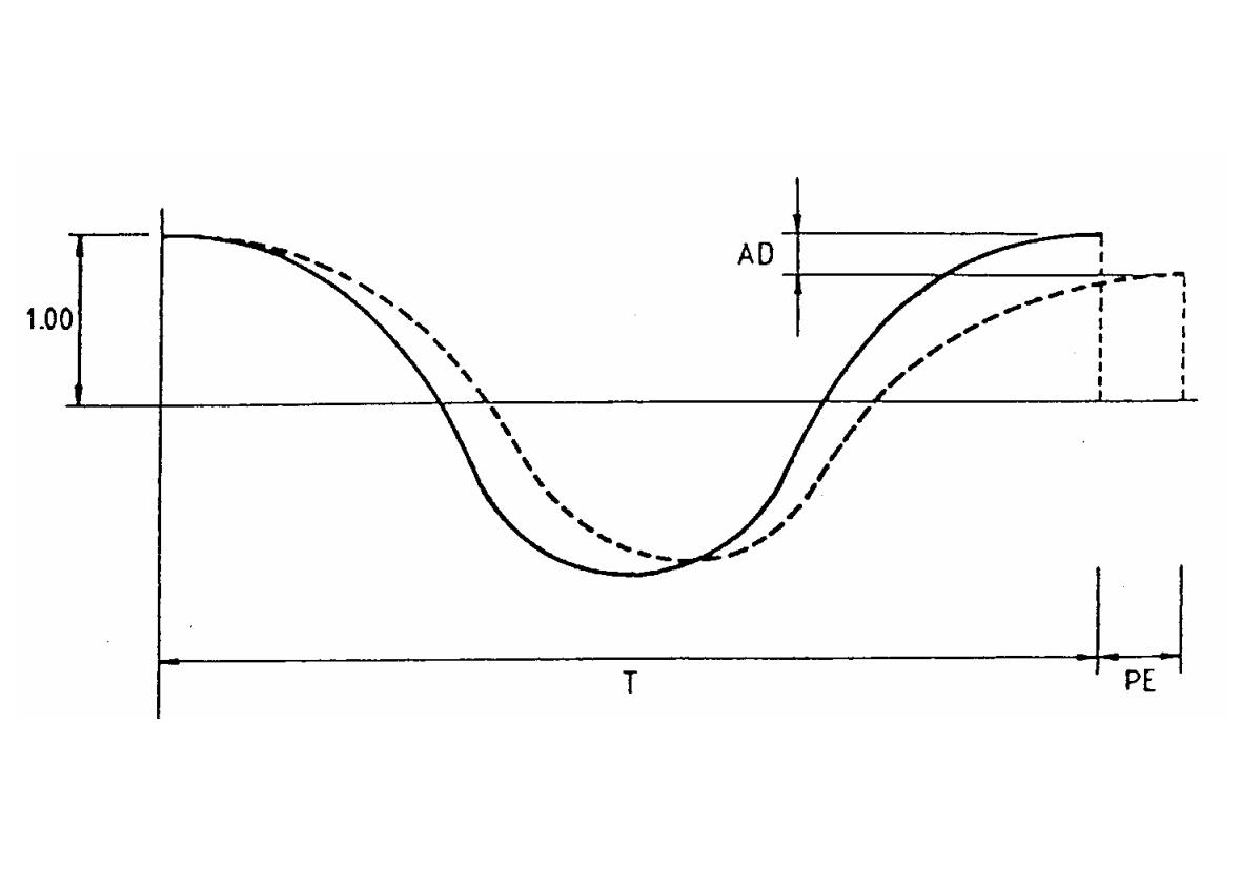
\includegraphics[width=0.75\textwidth]{pontatlansag.pdf}
\caption{A numerikus integrálás pontatlanságai \cite{gyorgyi}.}
\label{fig:pont}
\end{figure}
 
Az ábrán "T" a periódusidőt jelenti. A folytonos vonal a valós elmozdulást, a szaggatott pedig a numerikus számításból adódó elmozdulást  jelöli.


\subsection{Időlépéses módszerek stabilitásának vizsgálata}

{\ }

A numerikus számításoktól elvárjuk, hogy stabilak legyenek. A stabilitás csillapítatlan szabadrezgés esetén szemléltethető a legjobban. Az  integráló formulát akkor tekinthetjük stabilnak, ha a rendszer beáll valamilyen állandósult rezgésre. Ha  azonban a megoldás azt eredményezi, hogy a rendszerben egyre növekvő elmozdulások keletkeznek, az integráló eljárás az adott paraméterekkel nem nevezhető stabilnak. A követezőkben bemutatom az általános stabilitásvizsgálatot.

Először definiáljuk $t_i$ és $t_{i+1}$ időpontpeli mozgásjellemzőket a következő vektorokkal:
\begin{align*}
\mathbf{\hat{u}}_i & = \left[ \begin{array}{cc} \mathbf{u}_i \\ \mathbf{\dot{u}}_i \end{array} \right], & \mathbf{\hat{u}}_{i+1} & = \left[ \begin{array}{cc} \mathbf{u}_{i+1} \\ \mathbf{\dot{u}}_{i+1} \end{array} \right].
\end{align*}
Minden eljárás esetében felírható egy általános összefüggés a $t_{i+1}$ és $t_i$ időpontbeli mozgásjellemzők között:
\begin{equation}
\label{stab}
\mathbf{\hat{u}}_{i+1} = \mathbf{A}\mathbf{\hat{u}}_i.
\end{equation}
Ekkor az $\mathbf{\hat{u}}_t$ vektorban a $t+\Delta{t}$ időponthoz tartozó érték számításához szükséges jellemzők szerepelnek. A kifejezés felírható a következő alakban:
\begin{equation*}
\mathbf{\hat{u}}_{n} = \mathbf{A}\mathbf{\hat{u}}_{n-1} = \mathbf{A}^{n}\mathbf{\hat{u}}_1.
\end{equation*}
Az $\mathbf{A}^n$ mátrix felírható
\begin{equation*}
\mathbf{A}^n = \mathbf{P}\mathbf{J}^n\mathbf{P}^{-1},
\end{equation*}
alakban, ahol a $\mathbf{P}$ mátrixban az $\mathbf{A}$ mátrix sajátvektorai, a $\mathbf{J}$ mátrix főátlójában pedig az $\mathbf{A}$ mátrix sajátértékei helyezkednek el. A kifejezés stabilitásának feltétele, hogy az $\mathbf{A}^n$ mátrix ne a végtelenhez konvergáljon, tehát a sajátértékek  abszolút értéke maximum 1 legyen:
\begin{equation}
\rho\left(\mathbf{A}\right) = max|\lambda_k| \leq 1.
\label{stab felt}
\end{equation}  

A \eqref{stab felt} kifejezést az egyes eljárások esetében megoldva definiálhatjuk a feltételes és a feltétel nélküli stabilitást. Ha azt kapjuk eredményül, hogy az integrálási lépésköz frekvenciafüggő, akkor feltételes stabilitásról beszélhetünk. Ez többnyire az explicit eljárásokra jellemző. Amikor viszont a stabilitási vizsgálatot elvégezve az eredmény nem függ a sajátkörfrekvenciától, az eljárást feltétel nélkül stabilnak nevezzük. Ezeknél az eljárásoknál a stabilitás valamilyen integrálási paraméter függvénye. Többnyire ebbe a csoportba  az implicit módszerek tartoznak. Kivételt képez a Chen-Ricles algoritmus, ami egy feltétel nélkül stabil explicit eljárás.  


\subsection{Időlépéses módszerek alkalmazása modálanalízis esetén}

{\ }

Nagyméretű feladatok esetén előfordulhat olyan eset, hogy a modálanalízis és a numerikus integrálás együttes alkalmazása válik szükségessé \cite{gyorgyi}. 

Arányos csillapítás esetén az ekvivalens csillapítási mátrix felírható formális alakban:
\begin{equation}
\label{csill}
\mathbf{C} = \frac{\gamma}{\omega_{0r}}\mathbf{K},
\end{equation}
ahol $\omega_{0r}$ az $r$-edik sajátkörfrekvencia. A \eqref{csill} kifejezést formálisan behelyettesítve a \eqref{rezgegy} mátrix-differenciálegyenletbe:
\begin{equation*}
\mathbf{M}\mathbf{\ddot{x}}(t)+\frac{\gamma}{\omega_{0r}}\mathbf{K}\mathbf{\dot{x}}(t)+\mathbf{K}\mathbf{x}(t) = \mathbf{p}(t).
\end{equation*}
Ilyenkor a feladat csak modálanalízis és numerikus integrálás együttes alkalmazásával kezelhető.

Bevezetve az $\mathbf{x} = \mathbf{V}\mathbf{y}(t)$ összefüggést, ahol $\mathbf{V}$ a sajátvektorok mátrixa, és megszorozva az egyenletet balról $
\mathbf{V}^T$ mátrixszal az alábbi egyenletet kapjuk:
%
\begin{equation*}
\mathbf{V}^T\mathbf{M}\mathbf{V}\mathbf{\ddot{y}}(t)+\frac{\gamma}{\omega_{0r}}\mathbf{V}^T\mathbf{K}\mathbf{V}\mathbf{\dot{y}}(t)+\mathbf{V}^T\mathbf{K}\mathbf{V}\mathbf{y}(t) = \mathbf{V}^T\mathbf{q}(t)
\end{equation*}
%
Ekkor a mátrix-differenciálegyenlet n számú független egyszabadságfokú rezgés differenciálegyenletére esik szét:
%
\begin{equation*}
\ddot{y}_r(t)+\gamma\omega_{0r}\dot{y}_r(t)+\omega_{0r}^2y_r(t) = \mathbf{v_r}^T\mathbf{q}(t) = f_r(t),
\end{equation*}
%
ahol $f_r(t)$ az idő tetszőleges függvénye. Egyszabadságfokú rendszerre is alkalmazhatók a numerikus integráló eljárások. A számítás $t = 0$ időpontban kezdődik. Az ehhez tartozó kezdeti feltételek:
\begin{align*}
%
y_{0r} & = \mathbf{v}_r^T\mathbf{M}\mathbf{x}_0, & \dot{y}_{0r} =  \mathbf{v}_r^T\mathbf{M}\mathbf{\dot{x}}_0,
\end{align*}
%
és $\ddot{y}_{0r}$ értékek az
%
\begin{equation*}
\ddot{y}_{0r}+\gamma\omega_{0r}\dot{y}_{0r}+\omega_{0r}^2y_{0r} =  f_r(0)
\end{equation*}
%
egyenletből számíthatók. Az egyes időlépésekben az $y_r(t_{i+1}) = y_{r,i+1}$ értékeket kiszámítva az elmozdulásvektor a sajátvektorok segítségével:
%
\begin{equation*}
\mathbf{u}_{i+1} = \sum_{r=1}^{n}\mathbf{v}_r{y}_{r,i+1}.
\end{equation*}

%Fontos kérdés modálanalízis nagyméretű feladatokra alkalmazásánál, hogy mennyi sajátvektort kell figyelembe venni.


\section{Időlépéses módszerek alkalmazása lineáris rendszerek vizsgálatára}\label{sec:idolepmsz}

{\ }

A lineáris  szerkezetek viselkedése jól ismert a különböző hatásokra, mozgásegyenleteik pedig a nemlineáris mozgásegyenletekhez képest jóval egyszerűbbek. Számos numerikus integráló eljárást fejlesztettek lineáris egyenletek megoldására. A következőkben a legfontosabb lineáris  módszereket ismertetem.

\subsection{Euler-Cauchy módszer}

{\ }

Az Euler-Cauchy-, vagy más néven explicit Euler-módszer \cite{nummat}, az elmozdulás görbéjét a $t_i$ és $t_{i+1}$ időpontok között a görbe $t_i$ pontbeli érintőjével közelíti. A módszert  szokás töröttvonalmódszernek is nevezni.

A sebesség függvénye felírható és átalakítható az alábbi módon:
\begin{align*}
\mathbf{\dot{u}}(t) & = f(\mathbf{u}), \\
\frac{d\mathbf{u}(t)}{dt} & = f(\mathbf{u}), \\
d\mathbf{u} & = f(\mathbf{u})dt.
\end{align*}
Az időbeni diszkretizálást követően  a sebesség változása a $\Delta{t}$ intervallumon, a $\Delta{t}$-ben magasabb rendű tagokat elhanyagolva:
\begin{equation}
\label{euler du}
\Delta{\mathbf{u}} = \Delta{t}f(\mathbf{u}).
\end{equation}
A \eqref{euler du} kifejezést felhasználva az elmozdulás a $t_{i+1}$ időpontban:
\begin{equation}
\label{euler ui1}
\mathbf{u}_{i+1}  = \mathbf{u}_i+\Delta{\mathbf{u}}_i,  = \mathbf{u}_i+\Delta{t}\mathbf{\dot{u}}_i.
\end{equation}

A \eqref{euler ui1} kifejezésből látszik, hogy a módszer explicit, mert a $t_i$ időpontbeli értékek ismeretében közvetlenül meghatározhatók a $t_{i+1}$ pontbeli közelítések. 

Az eljárás nem stabil, a közelítésnél egyre nagyobb hibák fognak adódni. A lokális hiba $t^2$-tel arányos.


\subsection{Runge-Kutta típusú módszerek}

{\ }

A Runge-Kutta típusú módszerek \cite{nummat} az egylépéses explicit Euler- módszer "finomításának" mondhatók. Az elmozdulás görbéjét a $t_i$ és $t_{i+1}$ pontok közötti osztópontokba húzott érintőkkel közelítjük, tehát egy időlépés alatt több lépésben számítjuk az elmozdulásgörbét.

A másodrendű módszerek (röviden RK2) közül a legegyszerűbb a javított explicit Euler-módszer: a $t = t_{i}+0.5\Delta{t} = t_{i+0.5}$ felezőpontban explicit Euler-módszerrel kiszámoljuk az $\mathbf{u}(t)$ pontos érték $\mathbf{u}_{i+0.5} = \mathbf{u}_i+0.5\Delta{t}\mathbf{\dot{u}}_i$ közelítését, majd ezzel az értékkel meghatározott irányban egy újabb explicit Euler-módszert írunk fel a teljes intervallumra. Az elmozdulás $t_{i+1}$ időpontban ekkor:
\begin{equation*}
\mathbf{u}_{i+1} = \mathbf{u}_i+ \Delta{t}\mathbf{\dot{u}}_{i+0.5}.
\end{equation*}
A lokális hiba RK2 módszernél $t^3$-nal arányos.

 A harmadrendű módszerek közül  (röviden RK3) az egyik módszer esetén $t = t_{i}+0.3\Delta{t} = t_{i+0.3}$ és $t = t_{i}+0.6\Delta{t} = t_{i+0.6}$ harmadolópontokban határozzuk meg a közelítő érintőket. Ebből a $t_{i+1}$ időpontra az elmozdulás:
\begin{equation*}
\mathbf{u}_{i+1} = \mathbf{u}_i+0.5\Delta{t}\mathbf{\dot{u}}_{i+0.3}+0.5\Delta{t}\mathbf{\dot{u}}_{i+0.6}.
\end{equation*}
A lokális hiba ekkor $t^4$-nel arányos.

Felírhatók magasabb rendű Runge-Kutta módszerek is. Minél magasabb rendű az alkalmazott módszer, annál pontosabb eredményt kaphatunk, viszont egy időlépés alatt annál több közbenső lépést kell kiszámolnunk. A gyakorlatban ezért általában a negyed- és ötödrendű módszer a legmagasabb, ami előfordulhat. Léteznek a programrendszerekben olyan beépített programok, amik  beágyazott módszereket alkalmaznak. Ezek lényege, hogy  kiszámolnak két különböző rendű Runge-Kutta módszert (pl. egy negyed- és egy ötödrendűt), és úgy választanak lépésközt, hogy a hiba az alacsonyabb rendű hibája legyen.

\subsection{Centrális differenciák módszere}

{\ }

A centrális differenciák módszerében \cite{gyorgyi} az elmozdulásvektorok függvényét a $t_{i-1}, t_i$ és $t_{i+1}$ időpontokhoz tartozó $\mathbf{u}_{i-1}, \mathbf{u}_i, \mathbf{u}_{i+1}$ vektorelemek értékein átmenő másodfokú parabolákkal közelítjük (lásd: \ref{fig:centdiff} ábra). Ekkor:
%
\begin{align*}
\label{centdiff_av}
\mathbf{\dot{u}}_i&=\frac{1}{2\Delta{t}}\left(\mathbf{u}_{i+1}-\mathbf{u}_{i-1}\right), \\
\mathbf{\ddot{u}}_i&=\frac{1}{\Delta{t}^2}\left(\mathbf{u}_{i+1}-2\mathbf{u}_i+\mathbf{u}_{i-1}\right).
\end{align*}
%
A differenciahányadosokat behelyettesítve a \eqref{rezgegyi} alatti mátrix-differenciálegyenletbe $\mathbf{u}_{i+1}$-re az alábbi összefüggést kapjuk:
%
\begin{equation}
\label{centdiff long}
\left(\frac{1}{\Delta{t}^2}\mathbf{M}+\frac{1}{2\Delta{t}}\mathbf{C}\right)\mathbf{u}_{i+1} = \mathbf{q}_{i}+\left(\frac{2}{\Delta{t}^2}\mathbf{M}- \mathbf{K}\right)\mathbf{u}_i+\left(\frac{1}{2\Delta{t}}\mathbf{C}-\frac{1}{\Delta{t}^2}\mathbf{M}\right)\mathbf{u}_{i-1}.
\end{equation}
%
Az egyenlet rövidebb alakban a következőképp írható fel:
\begin{equation}
\label{centdiff short}
\mathbf{\hat{M}}\mathbf{u}_{i+1} = \mathbf{\hat{q}}_i,
\end{equation}
%
ahol $\mathbf{\hat{M}}$ a hatékony tömegmátrix, $\mathbf{\hat{q}}_i$ pedig a hatékony tehervektor $t_i$ időpillanatban. A módszer az explicit eljárások közé tartozik.

\begin{figure}[h!]
\centering
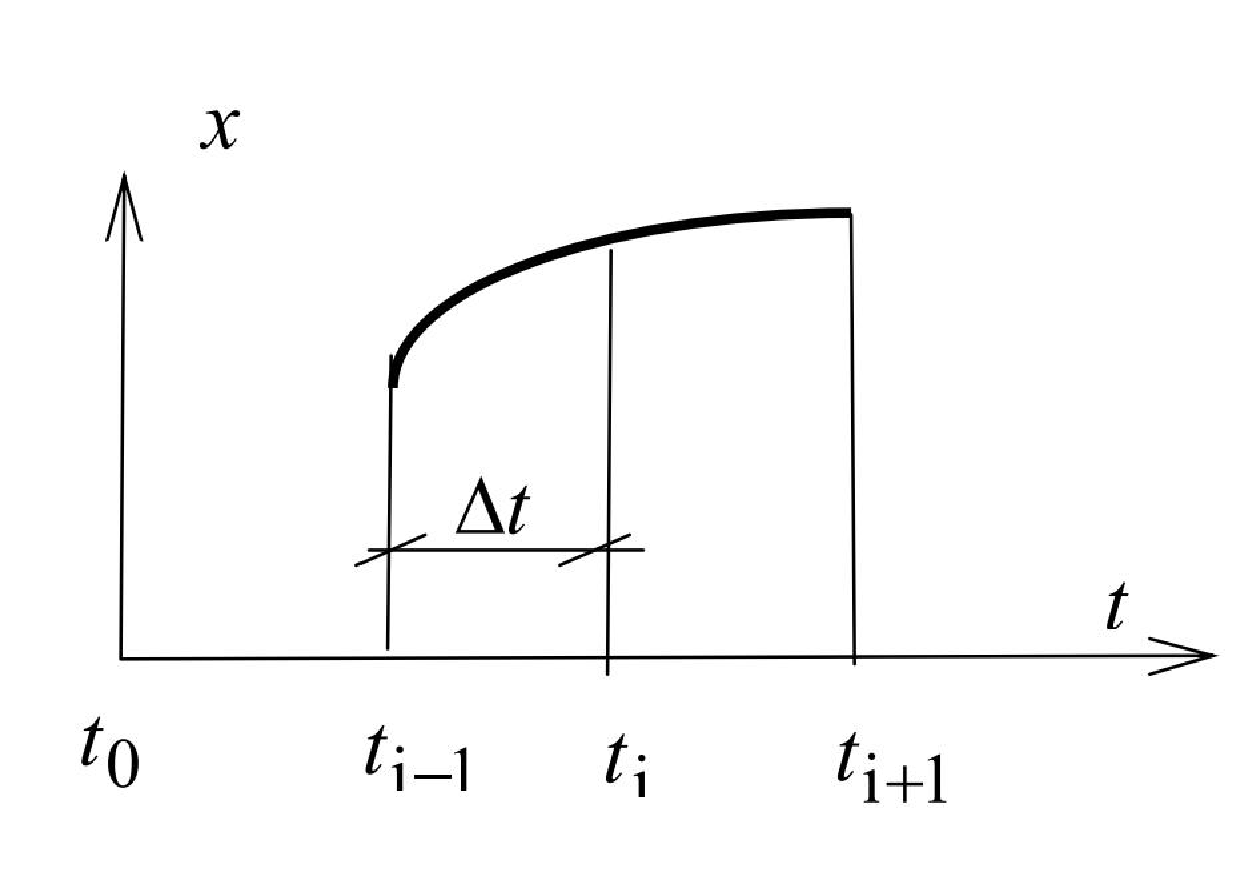
\includegraphics[width=0.5\textwidth]{centdiff.pdf}
\caption{Közelítő elmozdulások a centrális differenciák módszere szerint \cite{gyorgyi}.}
\label{fig:centdiff}
\end{figure}

Adott időpontban az elmozdulás kiszámításához mindig szükség van a megelőző két időpontbeli elmozdulásra, viszont a sebesség és elmozdulásvektorokat nem kell kiszámolni, ezeknek csak a kezdeti időpontbeli értékét használjuk. Az $\mathbf{u}_1$ vektor számításakor az $\mathbf{u}_{i-1}=\mathbf{u}_{-1}$ vektor helyére az
\begin{displaymath}
\label{u_min1}
\mathbf{u}_{-1}=\frac{(\Delta{t})^2}{2}\mathbf{\ddot{u}}_0-\Delta{t}\mathbf{\dot{u}}_0+\mathbf{u}_0
\end{displaymath}
%
összefüggés írható.

A eljárás feltételesen stabil, a szükséges időlépés frekvenciafüggő. A stabilitás feltétele:
\begin{equation*}
\Delta{t} \leq \frac{T_m}{\pi} = \frac{2}{\omega_0}.
\end{equation*}


\subsection{Newmark eljárás}\label{subsec:Newmark_lin}

{\ }

A Newmark eljárás \cite{gyorgyi} a $t_i$ és $t_{i+1}$ időpontok között egy $f(\tau)$ függvény szerinti gyorsulásváltozást feltételez. A gyorsulás ekkor a két időpont között egy $t_i+\tau = t_{i+\tau}$ időpontban:
\begin{equation*}
\mathbf{\ddot{u}}_{i+\tau} = \mathbf{\ddot{u}}_i+f(\tau)(\mathbf{\ddot{u}}_{i+1}-\mathbf{\ddot{u}}_i).
\end{equation*}
Az $f(\tau)$ értéke $\tau = 0$-nál zérus, míg $\tau = \Delta{t}$-nél 1. Az $f(\tau)$ függvénynek az eljárás stabilitásában van szerepe, és a továbbiakban $\gamma = \frac{1}{\Delta{t}}\int_0^{\Delta{t}}f(\tau)d\tau$ és $\beta = \frac{1}{\Delta{t}^2}\int_0^{\Delta{t}}\int_0^{\tau}f(\tau)d\tau$ paraméterekkel jellemezzük. 

Ezek után  a sebesség és gyorsulásvektor $\tau = \Delta{t}$ esetén a $t_{i+1}$ időpontban:
%
\begin{subequations}
\begin{align}
\mathbf{\dot{u}}_{i+1}& =  \mathbf{\dot{u}}_i+[(1-\gamma)\Delta{t}]\mathbf{\ddot{u}}_i+(\gamma\Delta{t})\mathbf{\ddot{u}}_{i+1},   \label{newmark1}\\ 
\mathbf{u}_{i+1}& =  \mathbf{u}_i+\Delta{t}\mathbf{\dot{u}}_i+\left[(0.5-\beta)
(\Delta{t})^2\right]\mathbf{\ddot{u}}_i+\left[\beta(\Delta{t})^2\right]\mathbf{\ddot{u}}_{i+1}. \label{newmark2}
\end{align}
\end{subequations}
% 
Ezeket behelyettesítve az \eqref{rezgesegy} alatti mátrix-differenciálegyenletet az i+1-dik időlépésben teljesítő \eqref{rezgegyi+1} egyenletbe, $\mathbf{u}_{i+1}$-re az alábbi összefüggést kapjuk:
%
\begin{equation}
\label{newmark long}
\begin{split}
\left(\mathbf{K}+\frac{1}{\beta\Delta{t}^2}\mathbf{M}+\frac{\gamma}{\beta\Delta{t}}\mathbf{C}\right)\mathbf{u}_{i+1} = \mathbf{q}_{i+1}+\mathbf{M}\left[\frac{1}{\beta\Delta{t}^2}\left(\mathbf{u}_i+\mathbf{\dot{u}}_i\Delta{t}\right)+\left( \frac{1}{2\beta}-1\right)\mathbf{\ddot{u}}_i\right]        \\ +\mathbf{C}\left[\frac{\gamma}{\beta\Delta{t}}\mathbf{u}_i+\left(\frac{\gamma}{\beta}-1\right)\mathbf{\dot{u}}_i+\left(\frac{\gamma}{2\beta}-1\right)\Delta{t}\mathbf{\ddot{u}}_i\right].
\end{split}
\end{equation}
%
Rövidebb alakban:
\begin{equation}
\label{newmark short}
\mathbf{\hat{K}}\mathbf{u}_{i+1} = \mathbf{\hat{q}}_{i+1},
\end{equation}
% 
ahol $\mathbf{\hat{K}}$ a hatékony merevségi mátrix, $\mathbf{\hat{q}}_{i+1}$ pedig a hatékony tehervektor a $t_{i+1}$ időpillanatban. Az együtthatómátrix lineáris szerkezet esetén időben állandó, ekkor a számítását és invertálását elég egyszer elvégezni.

\begin{figure}[h!]
\centering
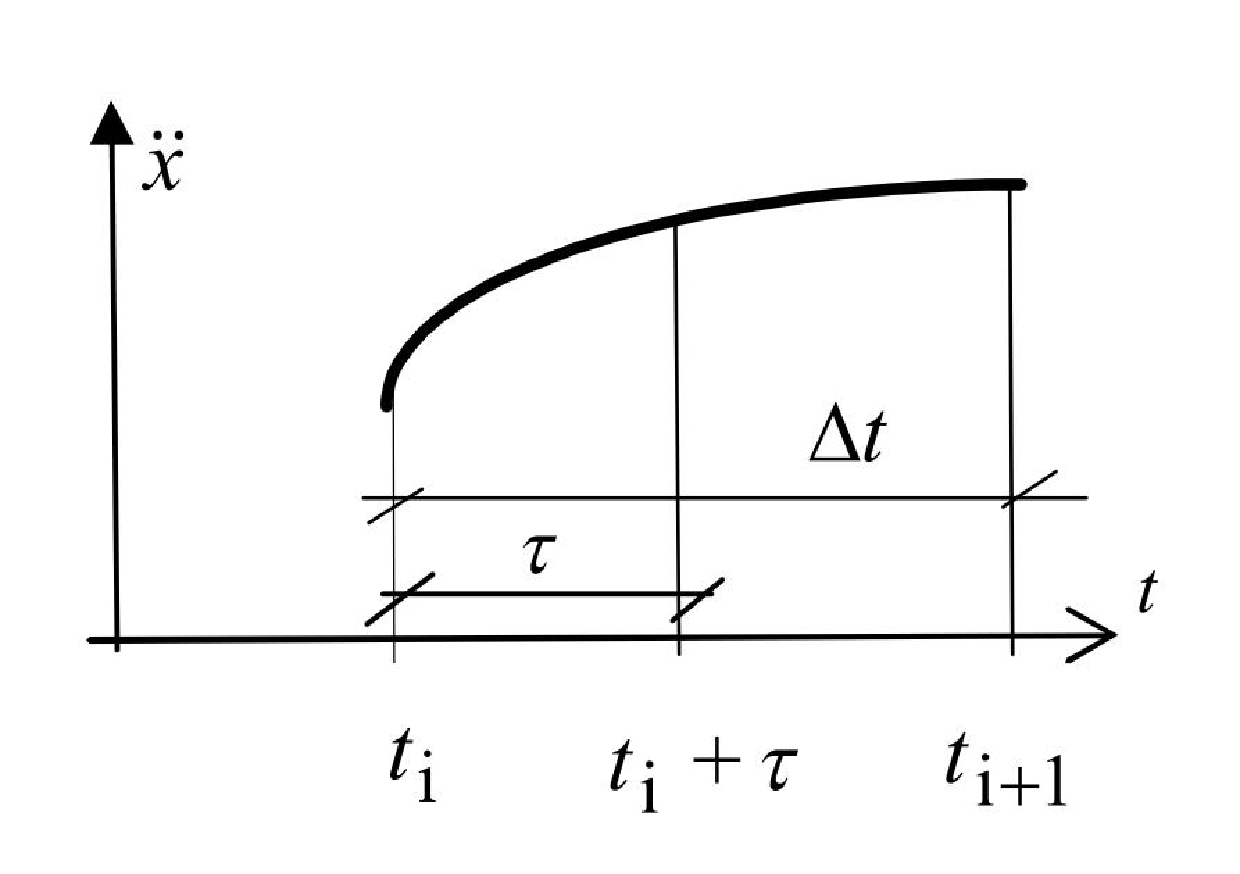
\includegraphics[width=0.45\textwidth]{newmark.pdf}
\caption{A Newmark eljárásnál feltételezett gyorsulás \cite{gyorgyi}.}
\label{fig:newmark}
\end{figure}

Az eljárás implicit, mivel a \eqref{newmark2} egyenlet alapján az i+1-dik  időpontbeli elmozdulás meghatározásához az i+1-dik  időpontbeli gyorsulásra is szükség van.

A $\gamma$ és $\beta$ paraméterek értékétől függően megkülönböztetünk néhány speciális esetet\cite{chopra,crcontthe}. Ha $(\gamma,\beta)=(1/2,1/4)$, akkor két időlépés között a gyorsulás konstans, és az átlagos értékkel egyezik meg, $(\gamma,\beta)=(1/2,1/6)$ értékpár esetén pedig lineáris a gyorsulás. A $(\gamma,\beta)=(1/2,0)$ esetet explicit Newmark eljárásnak nevezzük.

\begin{figure}[h!]
\centering
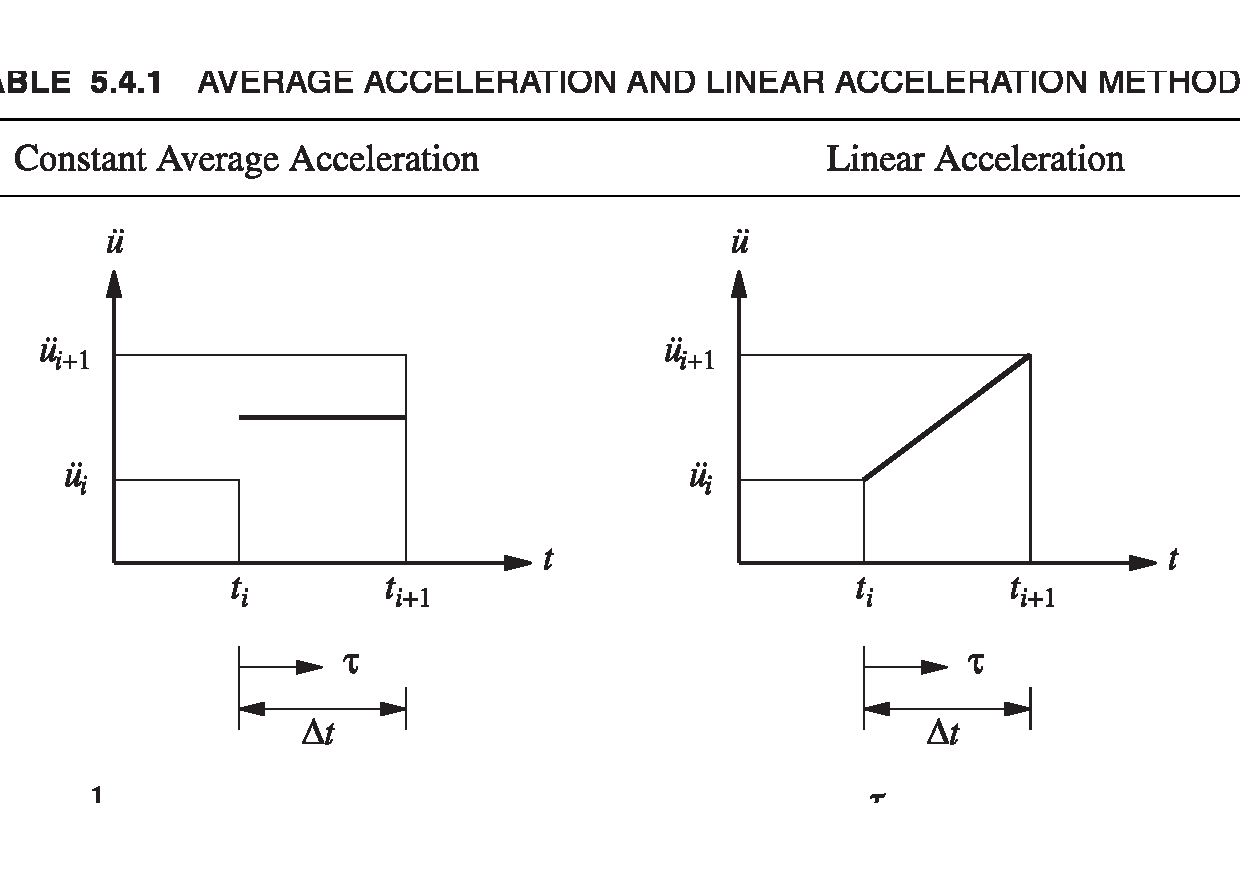
\includegraphics[trim = 0mm 15mm 0mm 20mm, clip, width=\textwidth]{newmark_spec.pdf}
\caption[Konstans átlagos gyorsulás és lineáris gyorsulás feltételezése]{Konstans átlagos gyorsulás (Constant Average Acceleration) és lineáris gyorsulás (Linear Acceleration) feltételezése \cite{chopra}.}
\label{fig:newmark spec}
\end{figure}

Az eljárás stabilitása és pontossága a $\gamma$ és $\beta$ paraméterek függvénye \cite{chopra}. A stabilitás feltétele tetszőleges $\gamma$-ra és $\beta$-ra a következő egyenlet teljesülése:
\begin{equation*}
\frac{\Delta{t}}{T_m}\leq\frac{1}{\pi\sqrt{2}}\frac{1}{\sqrt{\gamma-2\beta}}.
\end{equation*}
 Az eljárás feltétel nélkül stabil, ha
\begin{equation*}
\gamma\geq\frac{1}{2}, \qquad \beta\geq\frac{1}{4}\left(\frac{1}{2}+\gamma\right)^2, 
\end{equation*}
mivel a feltétel ekkor
\begin{equation*}
\frac{\Delta{t}}{T_m}<\infty.
\end{equation*}
Lineáris gyorsulás esetén  az egyenlőtlenségbe behelyettesítve
\begin{equation*}
\frac{\Delta{t}}{T_m}\leq0.551 
\end{equation*}
feltétel adódik az időlépés nagyságára, azonban ennél az eljárás pontossága érdekében a korábban ismertetett \eqref{dt max} képlet alapján kisebb lépésközt érdemes használni.

\subsection{Hilbert-Hughes-Taylor módszer}

{\ }

A Hilbert-Hughes-Taylor (továbbiakban HHT-$\alpha$ \cite{hht, hht_wiki}) módszer a Newmark eljárás módosítása. Alapja a Newmark eljárásnál definiált \eqref{newmark1} és \eqref{newmark2} egyenlet - $\gamma$ és $\beta$ paraméterek ugyanazzal a jelentéssel bírnak -, de a \eqref{rezgegyi+1} egyenlet helyett az alábbi egyenletbe helyettesítünk:
\begin{equation}
\mathbf{M}\mathbf{\ddot{u}}_{i+1}+\alpha\mathbf{C}\mathbf{\dot{u}}_{i+1}+(1-\alpha)\mathbf{C}\mathbf{\dot{u}}_{i}+\alpha\mathbf{K}\mathbf{u}_{i+1}+(1-\alpha)\mathbf{K}\mathbf{u}_i=\mathbf{q}_{i+\alpha},
\end{equation}
tehát a \eqref{rezgesegy} egyenletet a $t_{i+\alpha} = (i+\alpha)\Delta{t}$ időpillanatban elégítjük ki.
Ekkor a \eqref{newmark long} egyenlet a következőképpen módosul:
\begin{equation}
\label{hht long}
\begin{split}
\left(\alpha\mathbf{K}+\frac{1}{\beta\Delta{t}^2}\mathbf{M}+\frac{\gamma}{\beta\Delta{t}}\alpha\mathbf{C}\right)\mathbf{u}_{i+1} = \mathbf{q}_{i+\alpha}+\mathbf{M}\left[\frac{1}{\beta\Delta{t}^2}\left(\mathbf{u}_i+\mathbf{\dot{u}}_i\Delta{t}\right)+\left( \frac{1}{2\beta}-1\right)\mathbf{\ddot{u}}_i\right]        \\ +\alpha\mathbf{C}\left[\frac{\gamma}{\beta\Delta{t}}\mathbf{u}_i+\left(\frac{\gamma}{\beta}-1\right)\mathbf{\dot{u}}_i+\left(\frac{\gamma}{2\beta}-1\right)\Delta{t}\mathbf{\ddot{u}}_i\right]-(1-\alpha)\mathbf{C}\mathbf{\dot{u}}_i-(1-\alpha)\mathbf{K}\mathbf{u}_i,
\end{split}
\end{equation}
ahol
\begin{equation*}
\mathbf{q}_{i+\alpha} = \mathbf{q}(t_i+\alpha\Delta{t}).
\end{equation*}
%
Rövidebb alakban:
\begin{equation}
\label{hht short}
\mathbf{\hat{K}}_{\alpha}\mathbf{u}_{i+1} = \mathbf{\hat{q}}_{i+\alpha},
\end{equation}
ahol $\mathbf{\hat{K}}$ a hatékony merevségi mátrix, $\mathbf{\hat{q}}_{i+\alpha}$ pedig a hatékony tehervektor a $t_{i+\alpha}$ időpillanatban.


A módszer a Newmark eljáráshoz hasonlóan implicit. A stabilitás és pontosság a HHT-$\alpha$ módszernél is az integrálási paraméterektől függ, azonban $\gamma$ és $\beta$ függvénye $\alpha$-nak, melynek értéke $0.67$ és $1.00$ között változhat. Minél kisebb $\alpha$ értéke, annál pontosabb a módszer. Az $\alpha=1.0$ eset a Newmark eljárással egyezik meg. A módszer feltétel nélkül stabil, ha
\begin{equation*}
\beta = \frac{(2-\alpha)^2}{4}, \qquad \gamma = \frac{3}{2}-\alpha
 \end{equation*}

\subsection{Wilson-$\boldsymbol\theta$ eljárás}

{\ }

Az eljárás a $t$ és $t+\theta\Delta{t}$ időpontok között lineáris gyorsulásváltozást tételez fel, és szintén $t+\Delta{t}$ időpontban számítja az elmozdulást. A $\theta$ paraméternek az eljárás stabilitásában van szerepe.
A lineáris gyorsulásváltozás alapján egy $t+\tau$ időpontban felírhatók a gyorsulásvektorra, valamint a vektor integrálásával a sebességvektorra és az elmozdulásvektorra  vonatkozó összefüggések:
\begin{subequations}
\begin{align}
\mathbf{\ddot{u}}_{t+\tau} & = \mathbf{\ddot{u}}_{t}+\frac{\tau}{\theta\Delta{t}}\left(\mathbf{\ddot{u}}_{t+\theta\Delta{t}}-\mathbf{\ddot{u}}_t\right), \label{wilson_tau1}\\
\mathbf{\dot{u}}_{t+\tau} & = \mathbf{\dot{u}}_t+\mathbf{\ddot{u}}_t\tau+\frac{1}{2}\frac{\tau^2}{\theta\Delta{t}}\left(\mathbf{\ddot{u}}_{t+\theta\Delta{t}}-\mathbf{\ddot{u}}_t\right), \label{wilson_tau2}\\
\mathbf{u}_{t+\tau} & = \mathbf{u}_t+\mathbf{\dot{u}}_t\tau+\frac{1}{2}\mathbf{\ddot{u}}_t\tau^2+\frac{1}{6}\frac{\tau^3}{\theta\Delta{t}}\left(\mathbf{\ddot{u}}_{t+\theta\Delta{t}}-\mathbf{\ddot{u}}_t\right).\label{wilson_tau3}
\end{align}
\end{subequations}
A gyorsulásvektor és sebességvektor a $t+\theta\Delta{t}$ időpontban kifejezve:  
\begin{subequations}
\begin{align}
\mathbf{\ddot{u}}_{t+\theta\Delta{t}} & = \frac{6}{(\theta\Delta{t})^2}\left(\mathbf{u}_{t+\theta\Delta{t}}-\mathbf{u}_t\right)-\frac{6}{\theta\Delta{t}}\mathbf{\dot{u}}_t-2\mathbf{\ddot{u}}_t, \label{wilson theta a}\\
\mathbf{\dot{u}}_{t+\theta\Delta{t}} & = \frac{3}{\theta\Delta{t}}\left(\mathbf{u}_{t+\theta\Delta{t}}-\mathbf{u}_t\right)-2\mathbf{\dot{u}}_t-\frac{\theta\Delta{t}}{2} \mathbf{\ddot{u}}_t. \label{wilson theta v}
\end{align}
\end{subequations}
%
Mivel a gyorsulást lineárisnak feltételezzük $t$ és $t+\theta\Delta{t}$ időpontok között, az erőváltozást is lineárisnak kell tekintenünk. A $t+\theta\Delta{t}$ időponthoz tartozó erő:
\begin{equation*}
\mathbf{q}_{t+\theta\Delta{t}} = \mathbf{q}_t+\theta\left(\mathbf{q}_{t+\Delta{t}}-\mathbf{q}_t\right). 
\end{equation*}
Az \eqref{rezgesegy} alatti mátrix-differenciálegyenletet a $t+\theta\Delta{t}$ időpontra felírva $\mathbf{u}_{t+\theta\Delta{t}}$-re az alábbi egyenletet kapjuk:
\begin{equation}
\begin{split}
\label{wilson long}
\left(\mathbf{K}+\frac{3}{\theta\Delta{t}}\mathbf{C}+\frac{6}{(\theta\Delta{t})^2}\mathbf{M}\right)\mathbf{u}_{t+\theta\Delta{t}} = \mathbf{q}_t+\theta\left(\mathbf{q}_{t+\Delta{t}}-\mathbf{q}_t\right)\\+\mathbf{M}\left(\frac{6}{(\theta\Delta{t})^2}\mathbf{u}_t+\frac{6}{\theta\Delta{t}}\mathbf{\dot{u}}_t+2\mathbf{\ddot{u}}_t\right)+\mathbf{C}\left(\frac{3}{\theta\Delta{t}}\mathbf{u}_t+2\mathbf{\dot{u}}_t+\frac{\theta\Delta{t}}{2} \mathbf{\ddot{u}}_t\right).
\end{split}
\end{equation}
Rövidebb alakban felírva az egyenletet:
\begin{equation}
\label{wilson short}
\mathbf{\hat{K}}_{\theta}\mathbf{u}_{t+\theta\Delta{t}} = \mathbf{\hat{q}}_{t+\theta\Delta{t}},
\end{equation}
ahol  $\mathbf{\hat{K}}$ a hatékony merevségi mátrix, $\mathbf{\hat{q}}_{t+\theta\Delta{t}}$ pedig a hatékony tehervektor a $t_{i+\theta}$ időpillanatban. Az együtthatómátrix lineáris esetben időfüggetlen, tehát a számítások során elég egyszer előállítani és invertálni. Az eljárás implicit, mivel az elmozdulás a $t+\Delta{t}$ időpontban  függ a $t+\Delta{t}$ időpontban meghatározott erőtől.

Az $\mathbf{u}_{t+\theta\Delta{t}}$ ismeretében $\mathbf{\ddot{u}}_{t+\theta\Delta{t}}$ meghatározható a \eqref{wilson theta a} képlettel. Az $\mathbf{\ddot{u}}_{t+\theta\Delta{t}}$ valamint $t+\tau = t+\theta\Delta{t}$  a \eqref{wilson_tau1}, \eqref{wilson_tau2} és \eqref{wilson_tau3} képletekbe való behelyettesítésével számíthatjuk az $\mathbf{\ddot{u}}_{t+\Delta{t}}$, $\mathbf{\dot{u}}_{t+\Delta{t}}$ és az $\mathbf{u}_{t+\Delta{t}}$ vektorokat.

A eljárás feltétel nélküli stabilitása $\theta>1.37$ paraméter esetén biztosítható. A periódusidő meghosszabbodása függ az integrálási lépésköztől és a $\theta$ paramétertől, ennek optimális értéke  $1.40$.


\subsection{Chen-Ricles algoritmus}\label{subsec:cr}

{\ }

A Chen-Ricles (továbbiakban CR \cite{crcontthe}) algoritmus szintén a Newmark eljárásnál a \eqref{newmark1} és \eqref{newmark2} pontban ismertetett egyenletekből indul ki. Az eljárást elsősorban hibrid szimulációs módszerhez fejlesztették ki, de az algoritmus használható önálló numerikus számításként is. A sebességvektort és az elmozdulásvektort a következő összefüggések alapján számolja:  
\begin{subequations}
\begin{align}
\mathbf{\dot{u}}_{i+1} & = \mathbf{\dot{u}}_i+\boldsymbol\alpha_1\Delta{t}\mathbf{\ddot{u}}_i, \\
\mathbf{u}_{i+1} & = \mathbf{u}_i+\Delta{t}\mathbf{\dot{u}}_{i}+\boldsymbol\alpha_2\Delta{t}^2\mathbf{\ddot{u}}_i.
\end{align}
\end{subequations}
 Ezeket behelyettesítve a \eqref{rezgegyi+1} egyenletbe számítható a gyorsulásvektor. Az $\mathbf{\dot{u}}_{i+1}$ és $\mathbf{u}_{i+1}$ vektorok csak az $i$-dik időlépésben számolt értékektől függnek, tehát az eljárás explicit. A $t_{i+1}$ időpontbeli gyorsulást a \eqref{rezgegyi+1}  mozgásegyenletből számíthatjuk, $\mathbf{\dot{u}}_{i+1}$ és $\mathbf{u}_{i+1}$ vektorok behelyettesítésével:
\begin{equation}
\mathbf{\ddot{u}}_{i+1} = \mathbf{M}^{-1}(\mathbf{q}_{i+1}-\mathbf{C}\mathbf{\dot{u}}_{i+1}-\mathbf{K}\mathbf{u}_{i+1})
\end{equation} 
  
A módszer stabilitása a legtöbb explicit eljárással ellentétben frekvenciafüggetlen, azaz feltétel nélküli, ha  $\boldsymbol\alpha_1$ és  $\boldsymbol\alpha_2$ értékére teljesül a következő:
\begin{equation}
\label{cr alpha}
\boldsymbol\alpha_1 = \boldsymbol\alpha_2 = 4(4\mathbf{M}+2\Delta{t}\mathbf{C}+\Delta{t}^2\mathbf{K})^{-1}\mathbf{M}.
\end{equation}
Lineáris esetben a \eqref{cr alpha} mátrix időfüggetlen, ezért  előállítását elég egyszer elvégezni.


\section {Időlépéses módszerek alkalmazása nemlineáris rendszerek vizsgálatára}\label{sec:nl idolepmsz}

{\ }

A legtöbb építőmérnöki szerkezet nem csak lineárisan viselkedő elemeket tartalmaz, így viselkedésük leírására nem alkalmazhatók a hagyományos lineáris eljárások. Ilyenkor nemlineáris modellek segítségével sokkal pontosabb számításokat végezhetünk, ezáltal gazdaságosabb, jobban kihasznált szerkezeteket hozhatunk létre. Azonban a nemlineáris számítási módszerek sokkal bonyolultabbak, nehezebben programozhatók, és  a számítás hosszadalmasabb. 

A nemlineáris számításokra \cite{molnar} leggyakrabban a következők miatt lehet szükség:
\begin{itemize}
\item[--] a  felhasznált anyagok viselkedéséből adódó anyagi nemlinearitás (képlékenyedés: keményedés vagy 
lágyulás),
\item[--]  a szerkezet nagy alakváltozásai miatt létrejövő geometriai nemlinearitás hatása,
\item[--]  a szerkezet elmozdulásai miatt  módosuló  támaszrendszer hatása (peremfeltételi 
nemlinearitás).
\end{itemize}
Ezek viszonylag gyakran fordulnak elő az építőmérnöki gyakorlatban. A szerkezetek gazdaságossága miatt  például sokszor alkalmazunk olyan elemeket, amiknek kihasználjuk a képlékeny tartalékait is, a módosult támaszrendszer és a geometriai nemlinearitás kialakulása pedig fennáll a nagyobb dinamikus terhelések esetén, mint például a szélterhelés vagy a szeizmikus terhelés.

A nemlineáris számításokra vizsgált problémától függetlenül igaz, hogy a kiindulási feltételek jelentősen befolyásolják a vizsgálat eredményét, hogy nem alkalmazhatjuk a szuperpozíció elvét, és az, hogy  a teljes terheléstörténetet figyelembe kell vennünk. Ez utóbbi a dinamikus mozgásegyenletek esetében azt jelenti, hogy a $\mathbf{K}\mathbf{u}$ szorzat helyett egy elmozdulástól függő visszatérítő erőt használunk, amit minden időlépésben újra kell számolni. Ez sok esetben azt jelenti, hogy a megoldás együttható mátrixát minden időlépésben újra elő kell állítani és invertálni, ami elég hosszadalmas nagy szerkezetek esetében.

A rugalmas visszatérítő erő függvényének megválasztása a rendszerben alkalmazott nemlineáris anyagmodell alapján nehéz feladat, mert dinamikus terhelésre nem ismerünk jelenleg kellően pontos nemlineáris anyagmodellt. A visszatérítő erő számítása az egyes megoldási módszereknél lehet explicit, amikor  az $\mathbf{f}_{s,i}$ az $\mathbf{u}_i$-től függő mennyiség, illetve implicit, amikor az $\mathbf{f}_{s,i+1}$ az ismeretlen $\mathbf{u}_{i+1}$ függvénye. 

Nagyméretű szerkezetek vizsgálatánál a számítási sebesség szempontjából különösen fontos, hogy az explicit módszereknél kisebb időlépésköz használható az implicit eljárásokhoz képest. Viszont az implicit módszereknél, bár nagyobb időlépésköz a megengedett, és a szerkezet könnyebben kezelhető,  minden időlépésben iterációval közelítjük a megoldást. Az iterációk  számának  növelésével  javítható  az  eredmény  pontossága, azonban ez növeli a számításhoz szükséges időintervallumot is. Számítógépes programokban legtöbbször az implicit módszereket alkalmazzák. A következőkben a két legelterjedtebb módszernek, a centrális differenciák módszerének és a Newmark eljárásnak nemlineáris feladatokra való alkalmazását mutatom be.  





\subsection{Centrális differenciák módszere}

{\ }

A nemlineáris centrális differenciák módszerénél \cite{chopra} az elmozdulásvektorok függvényét a $t_{i-1}, t_i$ és $t_{i+1}$ időpontok között továbbra is  másodfokú parabolákkal közelítjük.

\begin{align*}
\label{centdiff_av}
\mathbf{\dot{u}}_i&=\frac{1}{2\Delta{t}}\left(\mathbf{u}_{i+1}-\mathbf{u}_{i-1}\right), \\
\mathbf{\ddot{u}}_i&=\frac{1}{\Delta{t}^2}\left(\mathbf{u}_{i+1}-2\mathbf{u}_i+\mathbf{u}_{i-1}\right).
\end{align*}
Az elmozdulásvektor pedig a következő alakban írható fel:
\begin{equation}
\mathbf{u}_{i+1} = \mathbf{u}_i+\Delta{\mathbf{u}}_i.
\end{equation}
A differenciahányadosokat behelyettesítve a \eqref{rezgegyi_nl} alatti mátrix-differenciálegyenletbe $\Delta{\mathbf{u}}_{i}$-re az alábbi összefüggést kapjuk:
\begin{equation}
\label{centdiff_nl}
\left(\frac{1}{\Delta{t}^2}\mathbf{M}+\frac{1}{2\Delta{t}}\mathbf{C}\right)\Delta{\mathbf{u}}_{i} = \mathbf{q}_i-\mathbf{f}_{s,i}+\left(\frac{1}{\Delta{t}^2}\mathbf{M}-\frac{1}{2\Delta{t}}\mathbf{C}\right)\Delta{\mathbf{u}}_{i-1}.
\end{equation}
Ezt szintén felírhatjuk rövidebb alakban:
\begin{equation}
\mathbf{\hat{M}}\Delta{\mathbf{u}}_i = \mathbf{\hat{q}}_i,
\end{equation}
ahol $\mathbf{\hat{M}}$ a hatékony tömegmátrix, $\mathbf{\hat{q}}_i$ pedig a hatékony tehervektor $t_i$ időpillanatban. A lineáris \eqref{centdiff long} és \eqref{centdiff short} egyenletekkel összehasonlítva az egyetlen különbség a $\mathbf{\hat{q}}_i$ vektorban található. 

Az $\mathbf{f}_{s,i}$ visszatérítő erő explicit módon származtatható a $t_i$ időpontbeli válaszból. Az együtthatómátrixban  nem szerepel a visszatérítő erő, ezért a vizsgálat ideje alatt állandó, és így elég azt  egyszer előállítani és invertálni, így az iteratív  nemlineáris eljárásokhoz képest a centrális differenciák módszere sokkal gyorsabb számítást tesz lehetővé. Ezáltal a módszer a legegyszerűbb nemlineáris eljárásnak tekinthető, viszont a többi eljáráshoz képest kevésbé pontos, ezért pontosabb számítást igénylő feladatokhoz általában nem ezt alkalmazzák.


\subsection{Statikus nemlineáris vizsgálat Newton-Raphson iteráció segítségével}

{\ }

 Implicit módszereknél, mint a Newmark eljárás, általában a kvázi-Newton-Raphson iterációs módszert \cite{chopra} használjuk a visszatérítő erő meghatározására, így a számítás nagy rendszereknél sokkal több időt vesz igénybe. A következőkben ismertetem a Newton-Raphson  iterációs eljárást statikus nemlineáris szerkezetek vizsgálatára.

A tehetetlenségi és csillapítási tulajdonságok elhanyagolásával a nemlineáris mozgásegyenlet a következő statikus problémaként írható fel:

\begin{equation*}
\mathbf{f}_s(\mathbf{u}) = \mathbf{q}.
\end{equation*}
Tehát a feladat a külső erőből adódó  elmozdulások meghatározása, úgy, hogy a erő és az elmozdulás kapcsolata, az $\mathbf{f}_s(\mathbf{u})$ visszatérítő erő függvény ismert a vizsgált rendszerben. A megoldáshoz iterációs eljárást alkalmazunk. Az iteráció $j$-edik lépésének elején  az ismert $\mathbf{u}^j$-ből számítható a kiegyensúlyozatlan erő:
\begin{equation*}
\mathbf{R} = \mathbf{q}-\mathbf{f}_s(\mathbf{u}^j)
\end{equation*}
 A visszatérítő erőt a   Taylor-sorba fejtjük a Newton-Raphson iteráció $j$-edik lépésében meghatározott $\mathbf{u}^j$ körül, majd a magasabbrendű tagokat elhanyagolva:
\begin{equation}
\label{f_s^j+1}
\mathbf{f}_s^{(j+1)} = \mathbf{f}_s^{(j)}+\mathbf{K}_T^{(j)}\Delta{\mathbf{u}}^{(j)} = \mathbf{q},
\end{equation}
ahol 
\begin{equation*}
\mathbf{K}_T^{(j)} = \left. \frac{\delta\mathbf{f}_s}{\delta\mathbf{u}} \right|_{\mathbf{u}^{(j)}},
\end{equation*}
az érintőmerevség mátrixa a visszatérítő erő $\mathbf{u}$ szerinti deriváltja az $\mathbf{u}^{(j)}$ helyen számítva, és $\Delta{\mathbf{u}}^{(j)} = \mathbf{u}^{(j+1)}-\mathbf{u}^{(j)}$  két egymást követő iteráció különbsége.

A \eqref{f_s^j+1} egyenletet megoldva megkapjuk  $\Delta{\mathbf{u}}^{(j)}$-t, ennek segítségével számíthatjuk $\mathbf{u}^{(j+1)}$ értékét.
%
\begin{equation}
\label{NR_u_j+1}
\mathbf{u}^{(j+1)} = \mathbf{u}^{(j)}+\Delta{\mathbf{u}}^{(j)} =  \mathbf{u}^{(j)}+\mathbf{K}_T^{(j)-1}(\mathbf{q}-\mathbf{f}_s^{(j)})
\end{equation}
Ezt tetszőleges iterációs lépésen keresztül számíthatjuk, az eredmények $\mathbf{u}$-hoz konvergálnak.  A gyorsabb konvergencia érdekében  a $\mathbf{q}$ terhet  $k$ darab $\Delta{\mathbf{q}}$ nagyságú teherlépcsőben szokták felvinni, ilyenkor egy-egy iteráció egy $\mathbf{u}_k$-hoz tart.

A módosított, kvázi-Newton-Raphson módszer abban különbözik az előbb leírtaktól, hogy a $\mathbf{K}_T$ érintőmerevséget nem számítjuk minden egyes  lépésben, csak teherlépcsőnként egyszer. A $k$-adik teherlépcsőn az $\mathbf{u}_{k}$ elmozduláshoz számított értékével vesszük figyelembe. Ennek eredményeképp a számítás sokkal egyszerűbb és gyorsabb, viszont a konvergencia lassabb lesz.

A megoldást minden iteráció után ellenőrizni kell, és ha valamelyik mennyiség eltérése egy hibahatáron belülre kerül, az iterációt nem érdemes tovább folytatni. Általában ennek ellenőrzésére a következő konvergenciakritériumokat használják:
\begin{itemize}
\item a maradék kiegyensúlyozatlan erő kisebb az előírtnál:
\begin{equation*}
\parallel \mathbf{R}^{(j)} \parallel \leq \epsilon_R
\end{equation*}
\item az elmozdulás változása kisebb az előírt értéknél:
\begin{equation*}
\parallel \Delta{\mathbf{u}}^{(j)} \parallel \leq \epsilon_u
\end{equation*}
\item az elmozdulásváltozást előidéző maradék kiegyensúlyozatlan erő által végzett munka kisebb az előírtnál:
\begin{equation*}
\frac{1}{2}\parallel \Delta{\mathbf{u}}^{(j)}\mathbf{R}^{(j)} \parallel \leq \epsilon_w
\end{equation*}
\end{itemize}

\subsection{Newmark eljárás}

{\ }

A  lineáris eljárásnál bemutatott \eqref{newmark1} és \eqref{newmark2} egyenletek továbbra is érvényesek:
%
\begin{align*}
\mathbf{\dot{u}}_{i+1}& =  \mathbf{\dot{u}}_i+[(1-\gamma)\Delta{t}]\mathbf{\ddot{u}}_i+(\gamma\Delta{t})\mathbf{\ddot{u}}_{i+1},   \\ 
\mathbf{u}_{i+1}& =  \mathbf{u}_i+\Delta{t}\mathbf{\dot{u}}_i+\left[(0.5-\beta)
(\Delta{t})^2\right]\mathbf{\ddot{u}}_i+\left[\beta(\Delta{t})^2\right]\mathbf{\ddot{u}}_{i+1}. 
\end{align*}
%
A nemlineáris Newmark eljárásnál \cite{chopra} a nemlineáris statikus vizsgálatnál bemutatott kvázi-Newton-Raphson iterációs módszert alkalmazzuk, azonban az eljárás során nem hanyagolhatjuk el a tehetetlenségi és csillapító tagokat.  Jelölje $\mathbf{\hat{f}}_{s,i+1}$ az $i$-edik időlépés $j$-edik iterációjában számított hatékony visszatérítő erőt. Ekkor:
%
\begin{equation*}
 \mathbf{\hat{f}}_{s,i+1} = \mathbf{M}\mathbf{\ddot{u}}_{i+1}+\mathbf{C}\mathbf{\dot{u}}_{i+1}+\mathbf{f}_{s,i+1} = \mathbf{q}_{i+1}.
\end{equation*}
 % 
 Az $\mathbf{\hat{f}}_{s,i+1}^{(j+1)}$ hatékony visszatérítő erő Taylor sorba fejtését elvégezve, az első két tag figyelembevételével a \eqref{f_s^j+1}   egyenlettel összeegyeztethető alakúra hozható a megoldás:
 %
 \begin{equation}
\label{Newmark_f_s^j+1}
\mathbf{\hat{f}}_{s,i+1}^{(j+1)} = \mathbf{f}_{s,i+1}^{(j)}+\mathbf{\hat{K}}_{T,i+1}\Delta{\mathbf{u}}^{(j)} = \mathbf{q}_{i+1},
\end{equation}
ahol
\begin{equation*}
\mathbf{\hat{K}}_{T,i+1} = \frac{\delta\mathbf{\hat{f}}_s}{\delta\mathbf{u}_{i+1}} = \frac{1}{\beta\Delta{t}^2}\mathbf{M}+\frac{\gamma}{\beta\Delta{t}}\mathbf{C}+\mathbf{K}_{T,i+1},
\end{equation*}
vagyis a hatékony érintőmerevség mátrixa a visszatérítő erő $\mathbf{u}_{i+1}$ szerinti deriváltja, és $\Delta{\mathbf{u}}^{(j)} = \mathbf{u}_{i+1}^{(j+1)}-\mathbf{u}_{i+1}^{(j)}$  két egymást követő iteráció különbsége.  

A \eqref{Newmark_f_s^j+1} egyenletet megoldva az egyes iterációs lépéseknél  megkapjuk $\Delta{\mathbf{u}}^{(j)}$-t, ennek segítségével számíthatjuk $\mathbf{u}_{i+1}^{(j+1)}$ értékét.
%
\begin{equation}
\label{Newmark_u_j+1}
\mathbf{u}_{i+1}^{(j+1)} = \mathbf{u}_{i+1}^{(j)}+\Delta{\mathbf{u}}^{(j)} =  \mathbf{u}_{i+1}^{(j)}+\mathbf{\hat{K}}_{T,i+1}^{-1}(\mathbf{q}_{i+1}-\mathbf{\hat{f}}_{s,i+1}^{(j)})
\end{equation}

Egy másik megközelítés alapján a gyorsulást fejezzük ki  a mozgásegyenletből. (A \ref{sec: nemlin progi} pontban bemutatásra kerülő nemlineáris megoldóprogramban mindkét megközelítés algoritmusa szerepel.)
\begin{equation}
\begin{split}
\left( \mathbf{M}+\Delta{t}\gamma\mathbf{C}+\Delta{t}^2\beta\mathbf{K}_{T,i+1}\right)\mathbf{\ddot{u}}_{i+1}^{(j+1)} = \mathbf{q}_{i+1} + \mathbf{r}_{i+1}^{(j)}-\mathbf{f}_{s,i+1}^{(j)}\\-\left(\mathbf{u}_i^{(j)}+\Delta{t}(1-\gamma)\mathbf{\ddot{u}}_i^{(j)}\right)\mathbf{C}-\left(\Delta{t}\mathbf{\dot{u}}_i^{(j)}+(0,5-\beta)\Delta{t}^2\mathbf{\ddot{u}}_i^{(j)}\right)\mathbf{K}_{T,i+1},
\end{split}
\end{equation}
ahol $\mathbf{r}_{i+1}^{(j)}$ a $j$-edik iterációnál keletkező, még kiegyensúlyozatlan erő. Az egyes iterációs lépésekben $\mathbf{u}_i^{(j)}$ elmozdulás- és $\mathbf{\dot{u}}_i^{(j)}$ sebességvektorokat a \eqref{newmark1} és \eqref{newmark2} egyenletekből, az $\mathbf{f}_{s,i+1}^{(j)}$ visszatérítő erőt pedig  $\mathbf{u}_i^{(j)}$ elmozdulásvektorból számíthatjuk.

Látható, hogy a nemlineáris Newmark eljárás a nemlineáris centrális differenciák módszeréhez képest sokkal bonyolultabb, és az iterációs számítás nagy rendszerek esetében jelentősen hosszabb. Viszont az eljárás előnyei közé tartozik, hogy feltétel nélkül stabil a \ref{subsec:Newmark_lin} pontban ismertetett integráló paraméterértékek esetén, illetve hogy  sokkal  pontosabb megoldásokkal szolgál, mint a centrális differenciák módszere. A Newmark eljárást sokszor alkalmazzák nemlineáris problémák megoldására.



\section{Az időlépéses módszerek alkalmazása}

{\ }

A tárgyalt lineáris és nemlineáris integráló formulákat a különböző, numerikus számításokat végző  programok használják közönséges differenciálegyenletek kezdetiérték feladatainak megoldására.  Különböző alkalmazási területeken más-más módszerek preferáltak. A legtöbbször a hagyományos eljárásokat, mint például  az Euler és a Runge-Kutta módszereket, illetve az építőmérnöki gyakorlatban a Newmark eljárást alkalmazzák.

Az általános matematikai számításokra használt szoftverek, mint például a MATLAB, a Maple vagy a Wolfram Mathematica általában a klasszikus formulákat alkalmazzák. Ezek vagy az utasításkészletbe beépített  függvényként találhatók, vagy könnyen beprogramozhatók. Léteznek a numerikus integráló formulákat tartalmazó függvénykönyvtárak is, amelyeket más programokban is lehet használni. A MATLAB programrendszerben az Ode rutinok alkalmazhatók közönséges differenciálegyenletek megoldására. Ezek között találhatók olyan egyszerűbb  módszerek, mint az Euler-Cauchy vagy a Runge-Kutta, vagy kicsivel bonyolultabb módszerek is, mint a beágyazott Runge-Kutta módszerek. Az Ode45 rutin például egy egylépéses, váltakozó lépésközű  beágyazott Runge-Kutta módszer, ami kiszámol egy negyed- és egy ötödrendű Runge-Kutta módszert, és úgy számol lépésközt, hogy a hiba a negyedrendű módszer hibája legyen. Az Ode megoldók nevében a számok sokszor azt jelzik, hogy hányad rendű módszereket alkalmaznak. 

A mérnöki gyakorlatban használt végeselemes programok általában vagy egy egyszerűbb explicit formulát alkalmaznak mint a centrális differenciák módszere, vagy egy pontosabb implicit formulát használnak, mint a Newmark eljárás. A centrális differenciák módszerét alkalmazzák például az LS/DYNA és az ABAQUS/Explicit szoftverek \cite{chopra}. Az explicit módszerek általában nem praktikusak nagyméretű szerkezetek elemzésére, mert  kisebb időlépések alkalmazását igénylik, viszont nagy előnyük, hogy jól használhatók a párhuzamosan több számítógépen futó számításokra. A végeselemes programok közül  azonban a legtöbb  a Newmark eljárást alkalmazza lineáris és nemlineáris számításokra, ilyen például az ANSYS és az AxisVM programcsomag. A NONSAP szoftver Wilson-$\boldsymbol\theta$ és Newmark eljárást is használ. Az implicit eljárások előnye, hogy nagyobb időlépésköz a megengedett, így a  nagy szerkezetek is könnyebben kezelhetők.

A mérnökszeizmológiai kutatásokhoz fejlesztett   végeselemes  szoftver  az OpenSEES (Open System for Earthquake Engineering Simulation). A programban az összes korábban ismertetett direkt integráló formula kiválasztható a dinamikus számításokhoz.

Az ismertetett integráló formulákat használva lineáris, nemlineáris és hibrid szimulációs programokat fejlesztettem MATLAB szoftver segítségével, melyeket a \ref{chap: lin+nemlin progi}. és a \ref{chap: hibrid progi}. fejezetekben mutatok be. A programokban nem  az Ode rutinokat, hanem saját megoldó algoritmusokat alkalmaztam. Azért döntöttem a MATLAB szoftver  mellett, mert fő jellemzői közé tartozik, hogy gyorsan számol nagy mátrixokkal, és hogy feladatspecifikusan alkalmazható, ezért laboratóriumi számításokhoz könnyen használható.


\chapter[Időlépéses program fejlesztése]{Időlépéses módszereket alkalmazó program fejlesztése}\label{chap: lin+nemlin progi}

{\ }

A következőkben az általam fejlesztett lineáris és nemlineáris időlépéses megoldó programokat mutatom be. A programokat MATLAB szoftverrel fejlesztettem, mert ez a programcsomag optimális választás a nagyméretű mátrixok gyors számítását igénylő feladatok esetében. Az egyes programokat eleve műveleti blokkokra osztottam, hogy a később bemutatásra kerülő hibrid módszert alkalmazó program elemeit könnyebb legyen beilleszteni. Az egyes műveleti blokkok a  feladatuk tekintetében megfeleltethetők egymásnak a  lineáris időlépéses megoldó, a nemlineáris időlépéses megoldó és a hibrid szimulációs  programban is. A lineáris és nemlineáris  időlépéses megoldó programok verifikálása a következő  fejezetben   olvasható.  Az egyes programok forráskódjait a Függelék tartalmazza.

\section{Lineáris feladatok megoldására fejlesztett program bemutatása}\label{sec: lin progi}

{\ }

A lineáris feladatok megoldására alkalmazható időlépéses megoldó módszereket használó program feladata elsősorban a \ref{sec:idolepmsz} pontban ismertetett időlépéses módszerek alkalmazása adott feladatokra, illetve az ezen algoritmusok összehasonlítása a módszer stabilitása, a megoldás pontossága valamint a számítások lefutásának sebessége szerint. A programban saját megoldó algoritmusokat használok.

\subsection{A program szerkezete}\label{subsec: lin prog szerk}

{\ }

A program folyamatábrája a \ref{fig:linprog} ábrán látható. Az indítást megelőzően szükséges  a szerkezeti rendszert leíró mátrixok és a kezdeti feltételek kézi megadása, valamint az egyes algoritmusokhoz tartozó integrálási paraméterek beállítása. Az indítást követően a program először létrehozza a  vizsgált rendszert leíró mátrixokat. Ezután egy felugró menüben ki kell választani az alkalmazni kívánt integráló algoritmust. A program ezt követően inicializálja a kiválasztott módszerhez tartozó integrálási paramétereket (ha van ilyen), majd létrehozza, illetve kiszámítja a módszerhez szükséges, a vizsgálat közben állandó (így csak egyszer előállítandó, esetleg invertálandó) segédmátrixokat, továbbá lefoglalja a helyet az időlépésenként  számítandó mátrixoknak. Ekkor egy for ciklusban az előre megadott vizsgálati időintervallumban, előre beállított lépésközökkel időlépésenként kiszámítja az elmozdulásvektort a kiválasztott módszer algoritmusával, majd el is tárolja azt. Végül a program kirajzolja az eredményül kapott diszkrét elmozdulásvektorokat a vizsgálat teljes időintervallumára.  
 
\begin{figure}[h!]
\centering
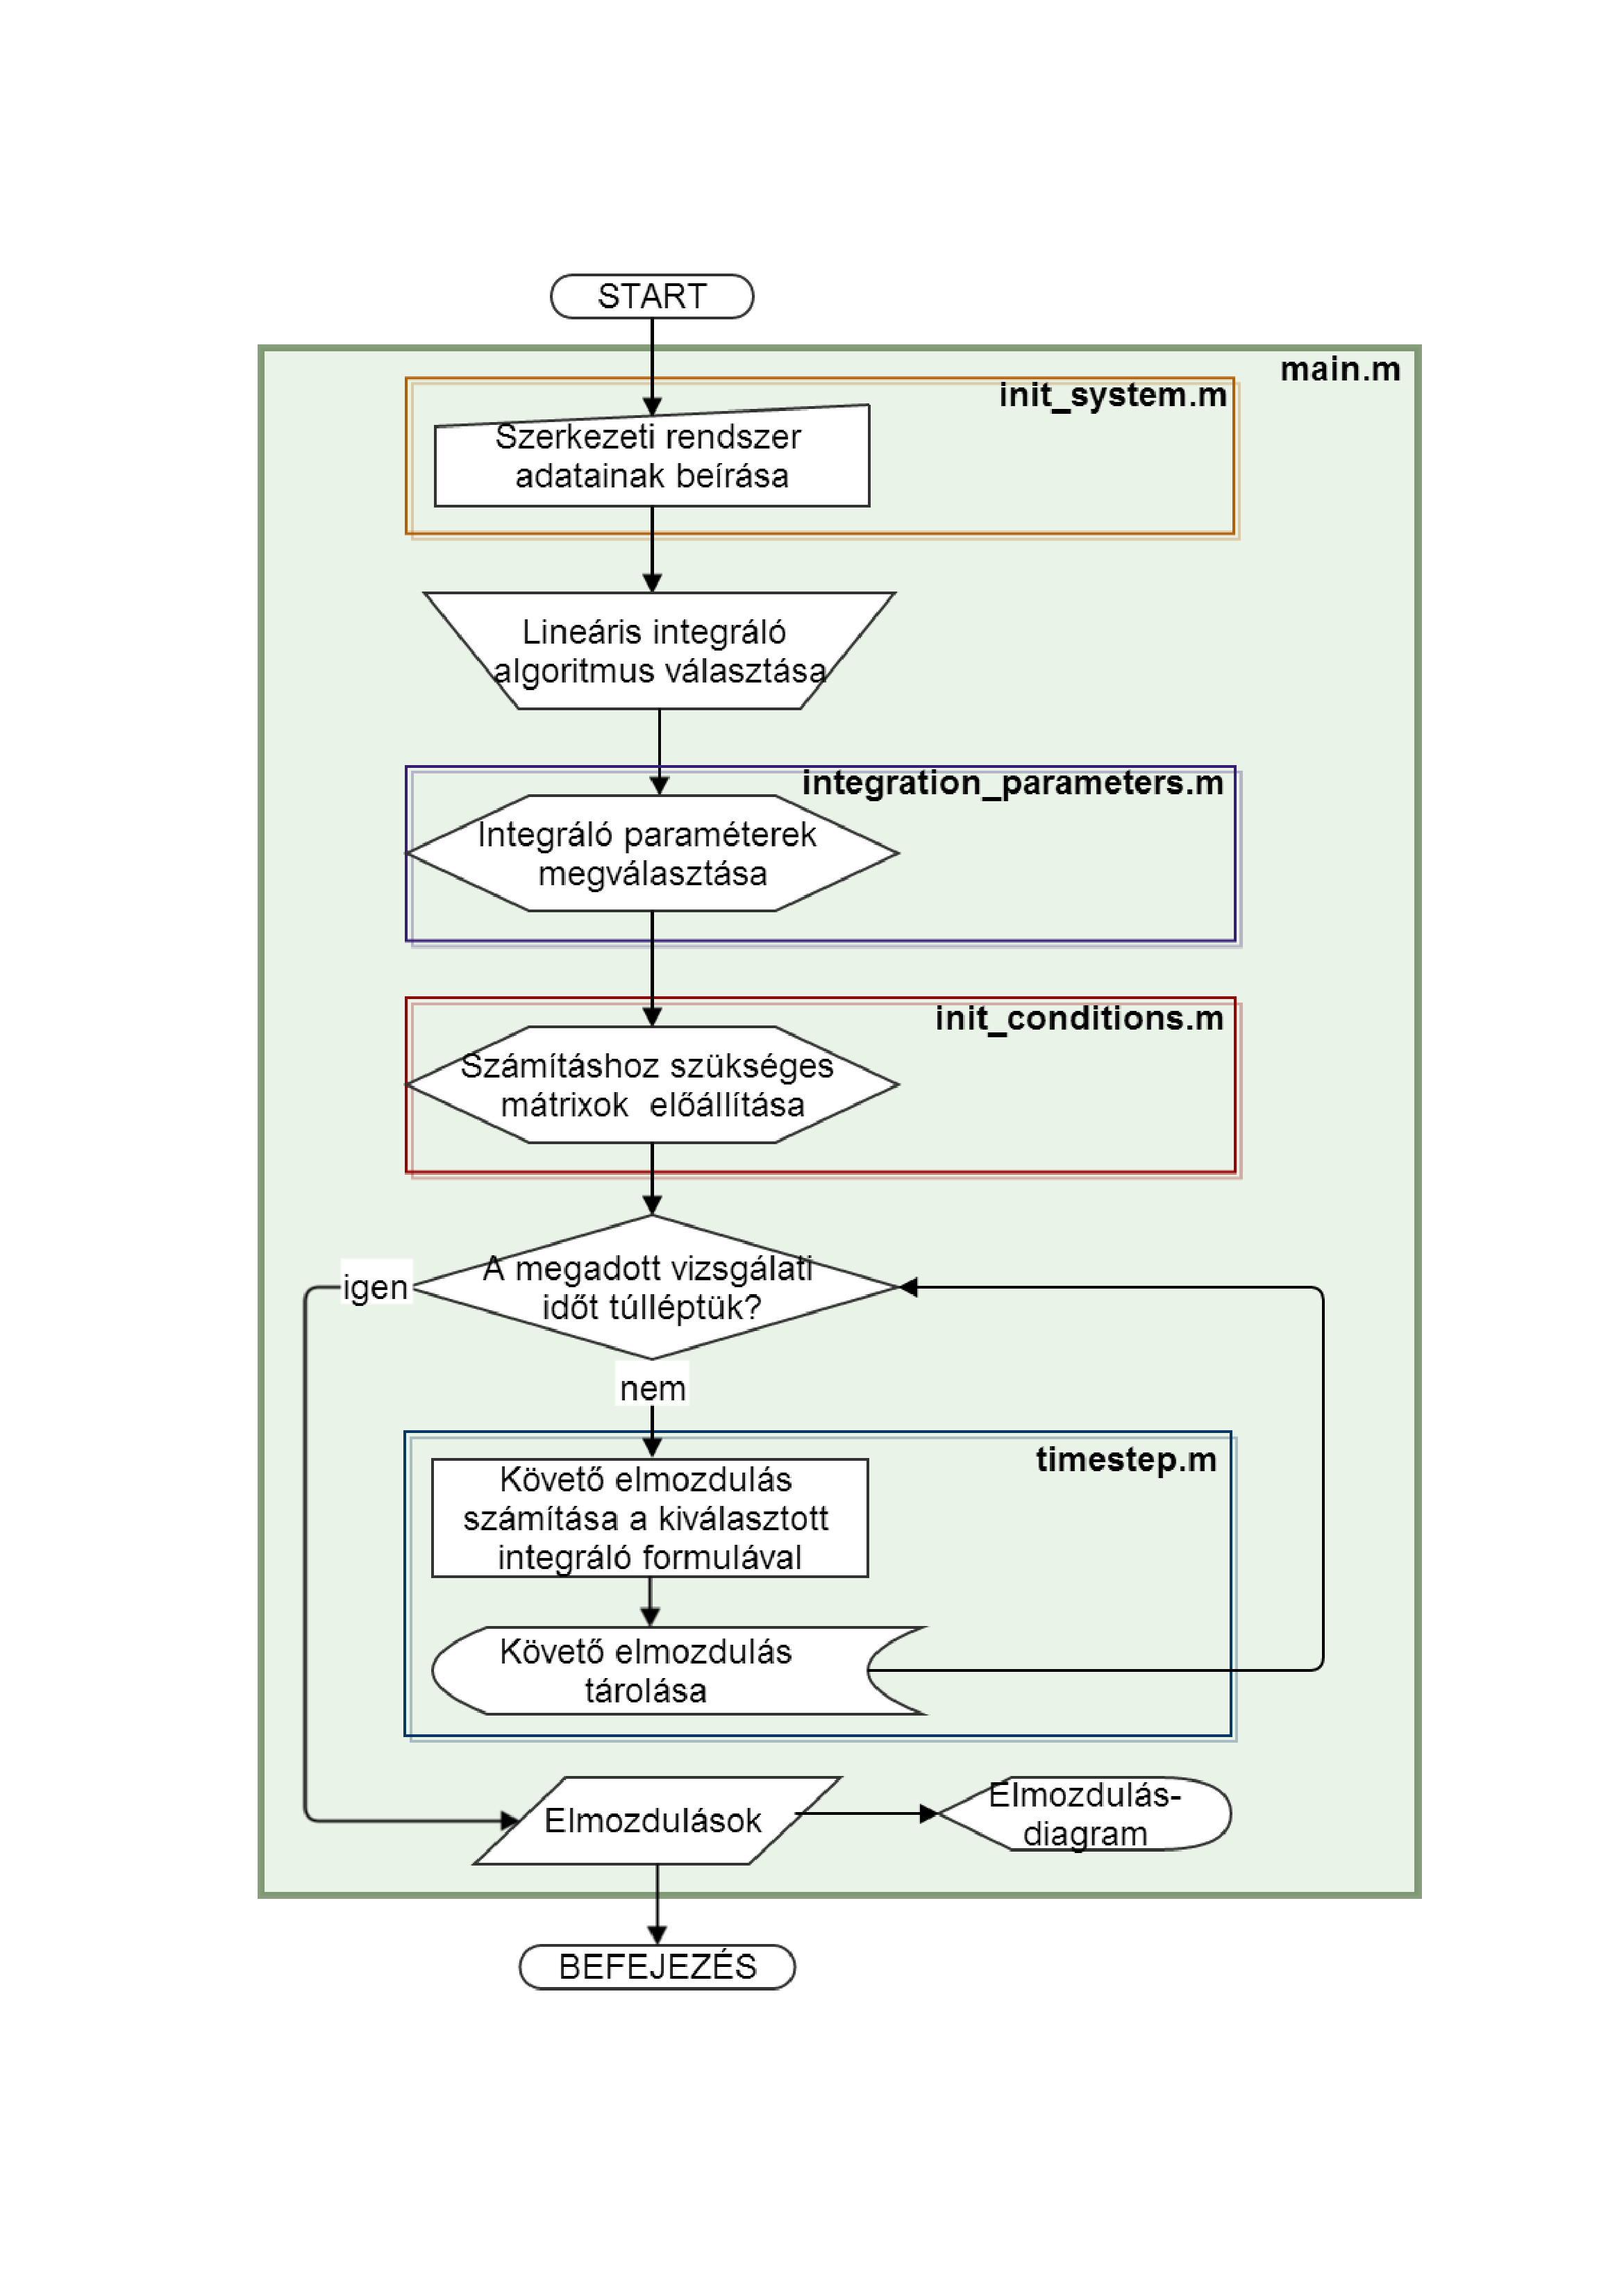
\includegraphics[trim = 0mm 50mm 0mm 50mm, clip, width=\textwidth]{linearis_folyamatabra.pdf}
\caption{A lineáris időlépéses megoldó program folyamatábrája.}
\label{fig:linprog}
\end{figure}

A program műveleti blokkokból áll. Teljes kódja a Függelék \ref{chap: függ linprog}. pontjában található. A szkript típusú \verb|main.m| fájl tartalmazza a műveleti parancssort és a beillesztett inicializáló és számító blokkokat egyaránt.  Először egy biztonsági törlés elvégzését követően meghívja az \verb|init_system.m| fájlt a szerkezet alapadatainak beolvasásához. A main tartalmazza a felugró menüt, amiben a numerikus algoritmust választhatjuk ki. A módszer kiválasztása után futtatja az \verb|integration_parameters.m| valamint \verb|init_conditions.m| szkripteket, melyek az algoritmus futásához szükséges előkészületeket végzik. Ezt követően egy for ciklusban hívja a \verb|timestep.m| fájlt az elmozdulások számításához, majd kirajzolja az eredményt egy elmozdulás-idő grafikonon. 

A szerkezetet leíró mátrixokat és a kezdeti feltételeket az \verb|init_system.m| fájlban kell megadni. Ezek a vizsgálat időtartama, a diszkrét időpillanatok lépésköze, a szerkezetet leíró tömeg-, merevségi és csillapítási mátrixok, a tehervektor, illetve az $\mathbf{u}_0$ és  $\mathbf{\dot{u}}_0$  kezdeti feltételek. Ha az adott feladatban szükséges, számítjuk a szerkezet sajátkörfrekvenciáit és sajátrezgésalakjait.

Az egyes módszerekhez tartozó integrálási paraméterek értékeit (ha van ilyen) az \verb|integration_parameters.m| fájlban lehet beállítani. Ezek a  Newmark eljárásnál  $\gamma$ és $\beta$, a Wilson-$\theta$ eljárásnál $\theta$, a HHT-$\alpha$ módszernél $\gamma$, $\beta$ és $\alpha$, valamint a CR algoritmus esetében $\boldsymbol\alpha_1$ és $\boldsymbol\alpha_2$ paraméterek. Az egyes módszerek stabilitásához szükséges értékeket kommentként feltüntettem.
 
Az \verb|init_conditions.m| szkript tartalmazza a helyfoglaló mátrixokat, mint az elmozdulás-, sebesség- és gyorsulásvektorok mátrixait, továbbá elvégzi az egyes módszerekhez szükséges előre elvégezhető mátrixszámításokat, például a hatékony tömeg- vagy merevségi mátrix invertálását. 

 A \verb|timestep.m| fájlban pedig  az elmozdulásvektorok számítására  és tárolására vonatkozó, minden időlépésben végrehajtandó parancsok találhatók a \ref{sec:idolepmsz} pontban ismertetett algoritmusok alapján.
 
A program használatát két példán keresztül mutatom be. Mindkét esetben csak az \verb|init_system.m| fájlt kell a feladathoz igazítani és a "main" paranccsal meghívni a főprogramot, majd kiválasztani az integrálási algoritmust. 


\subsection{A program használata gerjesztett rezgés vizsgálatára}\label{subsec:lingerj}

{\ }

Ezen a példán keresztül három dolgot prezentálok. Bemutatom, hogyan adhatunk meg a programban  gerjesztést, hogyan állíthatunk be egy lecsengő szakaszon csillapított szabadrezgést, valamint hogy hogyan vizsgálhatjuk a gerjesztés és a csillapítás hatását. 

\begin{figure}[h!]
\centering
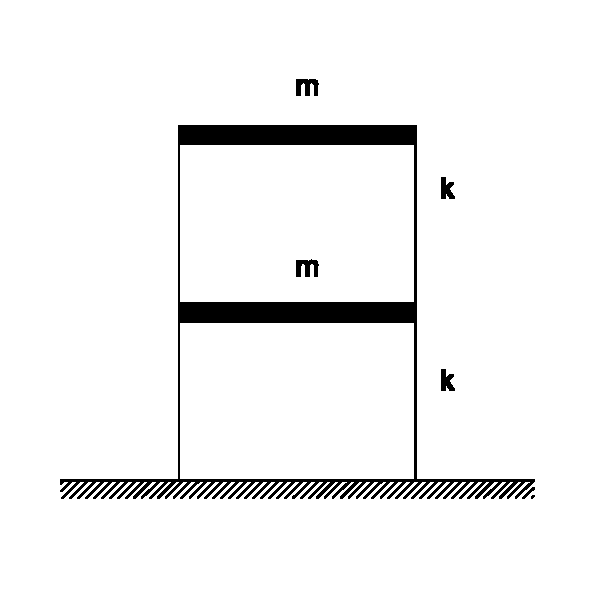
\includegraphics[width=0.4\textwidth]{ketzsintes.pdf}
\caption{A gerjesztéses példában vizsgált kétszintes keret.}
\label{fig:ketszabfok}
\end{figure}

A feladatban egy kétszabadságfokú rendszert gerjesztünk 6 másodpercig harmonikus gerjesztőerővel zérus kezdeti feltételek mellett, ekkor megszüntetjük a terhelést, és megvárjuk, amíg a szerkezet szabadrezgéssel lecsillapodik. Így az első szakaszban a  gerjesztés hatását, a második szakaszban pedig a csillapítás hatását tudjuk szemügyre venni. 

A modell egy kétszintes szerkezet, az egyes szintek tömege 45 tonna. Az egyes szintek merevsége 18000 kN/m. A  szerkezeten arányos csillapítást alkalmazunk, $\alpha$ és $\beta$ értékét úgy vesszük fel, hogy mindkét módban $\xi$ tényező értéke $5\%$ legyen. A lépésközt úgy választjuk meg, hogy megfeleljen az erre vonatkozó ökölszabálynak, és a 6 másodperc osztója legyen. Ez alapján a $dt = 0.02 s$ értéket vesszük fel. A teherfüggvény  az első 6 másodpercben mindkét szinten $10\sin(20t)$, utána zérus. A rendszert leíró bemeneti értékek képletekkel megadva a következők:
  \begin{align*}
  & t_{max}  = 12 sec  & & \Delta{t} = 0,02 sec   & \\
  & \mathbf{M}  = \left[\begin{array}{rr}  45 & 0 \\ 0 & 45 \end{array} \right]t   &  & \mathbf{K} = \left[\begin{array}{rr} 36 000 & -18 000 \\ -18 000 & 18 000 \end{array} \right]\frac{kN}{m}  &  \\
  & \mathbf{C}  = \alpha\mathbf{M}+\beta\mathbf{K}  &  & \xi = 0,05  & \\
  & \mathbf{q}_1  = \left[\begin{array}{c} 10 \\ 10 \end{array} \right]\sin{20t}  & & \mathbf{q}_2 = \left[\begin{array}{c} 0 \\ 0 \end{array} \right]  & \\
  & \mathbf{u}(0)  = \left[\begin{array}{c} 0 \\ 0 \end{array} \right]  & & \mathbf{\dot{u}}(0) = \left[\begin{array}{c} 0 \\ 0 \end{array} \right] & 
  \end{align*}
  %& \left[ \begin{array}{c} \alpha \\ \beta \end{array} \right] =  \left[ \begin{array}{c} \frac{2\xi\omega_{01}\omega_{02}}{\omega_{01}+\omega_{02}} \\ \frac{2\xi}{\omega_{01}+\omega_{02}} \end{array} \right], &

A programban ez alapján a  feladathoz tartozó \verb|init_system.m| fájl a következő: 
\lstinputlisting{"MATLAB/linear_system_312/init_system.m"}

A program az elmozdulásokat rajzolja ki az idő függvényében. A feladat Newmark eljárással való megoldása látható a \ref{fig:lingerjeredm_newmark} ábrán. A grafikon alapján elmondható, hogy a rendszer a gerjesztés alatt közel beáll egy állandósult rezgésre. Majd mikor megszüntetjük a gerjesztőerőt, kap egy nagyobb sebességet, aminek következtében megjelenik egy nagyobb kitérés. Ezt egy lecsengő szakasz követi, a csillapított szabadrezgésnek megfelelően. 
\begin{figure}[h!bt]
\centering
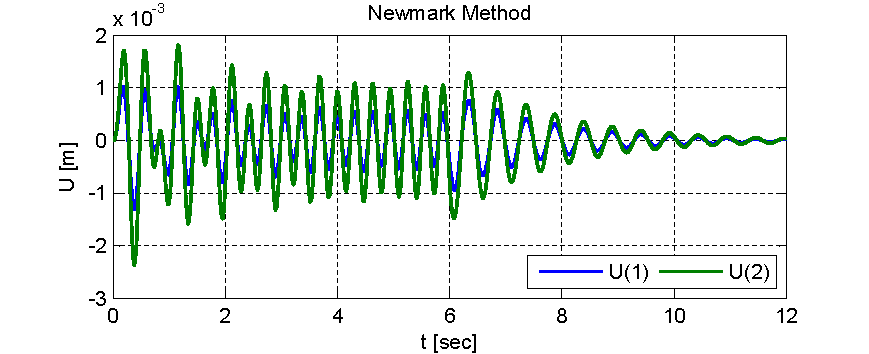
\includegraphics[width=\textwidth]{312_Newmark.pdf}
\caption{A \ref{subsec:lingerj} gerjesztett rezgéses példa elmozdulásai Newmark módszerrel.}
\label{fig:lingerjeredm_newmark}
\end{figure}

A számítás eredményei a többi módszerrel  a Függelék \ref{sec:függ_lingerj} pontjában találhatók. Ezeket a \ref{subsec: lin eredmény gerj} pontban hasonlítom össze.


\subsection{A program használata csillapítatlan szabadrezgés vizsgálatára}\label{subsec:szabrezg}

{\ }


E feladat célja az egyes módszerek jellemzése stabilitás és pontosság szempontjából. A csillapítás megszüntetésével az egyes módszerek stabilitása közelítő módon, numerikusan vizsgálható. Ahhoz, hogy az egyes rezgésmódok ne zavarják a szerkezet viselkedését, a  kezdeti feltételt valamelyik sajátalakként célszerű felvennünk.

Csillapítatlan szabadrezgés vizsgálatához a \ref{subsec:lingerj} pontban bemutatott kétszabadságfokú rendszert választottam. A feladatban a csillapítás és a tehervektor értéke egyaránt zérus, kezdeti feltételnek pedig az egyik sajátvektorral arányos kitérést adtam meg. A rendszert leíró bemeneti értékek a következőképp módosulnak a  gerjesztett rezgéshez képest:
  \begin{align*}
    & \mathbf{C}  = 0  & & \mathbf{q} = \left[\begin{array}{c} 0 \\ 0 \end{array} \right]  & \\
  & \mathbf{u}(0)  = \mathbf{v}_1  & & \mathbf{\dot{u}}(0) = \left[\begin{array}{c} 0 \\ 0 \end{array} \right]  & 
  \end{align*}
  
A bemeneti adatokat tartalmazó \verb|init_system.m| a következőkben módosul:
\lstinputlisting{"MATLAB/linear_system_313/init_system.m"}
 

\begin{figure}[h]
\centering
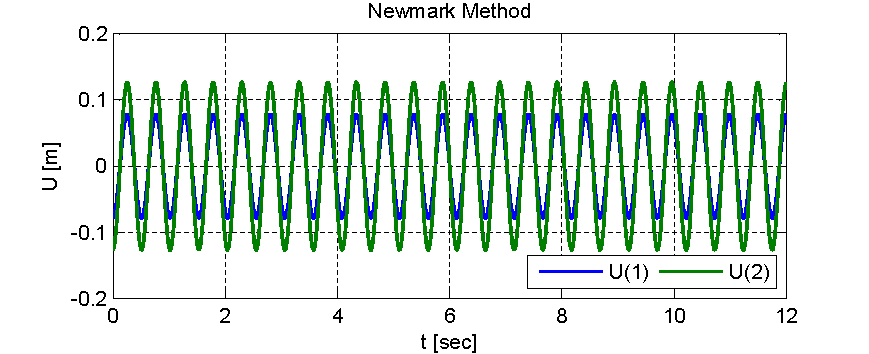
\includegraphics[width=\textwidth]{313_Newmark.pdf}
\caption{A \ref{subsec:szabrezg} szabadrezgéses példa elmozdulásai Newmark módszerrel.}
\label{fig:szabrezg_er_newmark}
\end{figure}

A \ref{fig:szabrezg_er_newmark} ábrán a feladat megoldásaként az elmozdulás-idő diagram látható, Newmark eljárással számítva. 
A pontosság szemléltetésére  a diagram nem feltétlenül alkalmas, mert az amplitúdó csökkenése a legtöbb esetben a görbén nem látszik egyértelműen, azonban a többi módszer eredményeivel összehasonlítva megfigyelhető rajta a periódusidő meghosszabbodása.  A programmal az elmozdulás-idő grafikon mellett kirajzoltattuk a mechanikai energia-idő diagramot, valamint a szerkezet két szintjének egymáshoz viszonyított  elmozdulását fázistérben. Erre egy-egy  példát  láthatunk Newmark módszerrel számítva a \ref{subsec: lin eredmény szabrezg} pontban.

 

\section{Nemlineáris feladatok megoldására fejlesztett program bemutatása}\label{sec: nemlin progi}

{\ }

A nemlineáris feladatok megoldására használható  programot szintén MATLAB programnyelven fejlesztettem. A program feladata  a \ref{sec:nl idolepmsz} pontban bemutatott időlépéses integráló formulák alkalmazása nemlineáris szerkezetekre, illetve ezen algoritmusok pontosságának. Ebben a programban is saját megoldó algoritmusokat használok.


\subsection{A program szerkezete}\label{subsec: nemlin prog szerk}
 
{\ }

A program folyamatábráját mutatja a \ref{fig:nemlinprog} ábra. A szerkezeti rendszer adatait és a kezdeti feltételeket a nemlineáris programban is az indítást megelőzően, kézzel kell  megadni. A Newmark algoritmusok használata esetén ekkor kell beállítani az integráló paraméterek értékét is. A program az indítását követően először létrehozza a szerkezeti rendszert leíró mátrixokat. Ezt követően egy felugró menüben kiválaszthatjuk az integráló algoritmust. Ekkor a Newmark algoritmusok esetében a integrálási paraméterek inicializálása következik, majd a választott módszer algoritmusához időlépésenként számítandó mátrixok helyfoglalása  és  a vizsgálat közben állandó kifejezések segédmátrixainak előállítása és tárolása történik. Ezután az időlépésekhez tartozó for ciklus következik. Minden lépésnél frissítjük a visszatérítő erőt és a Newmark formulák esetében az érintőmerevség értékét is, kiszámítjuk a következő időpillanatbeli elmozdulást, és eltároljuk az eredményt. Az utolsó lépés az eredményül kapott  elmozdulásvektor-diagramok kirajzolása a vizsgálat teljes idejére. 
 
\begin{figure}[h!]
\centering
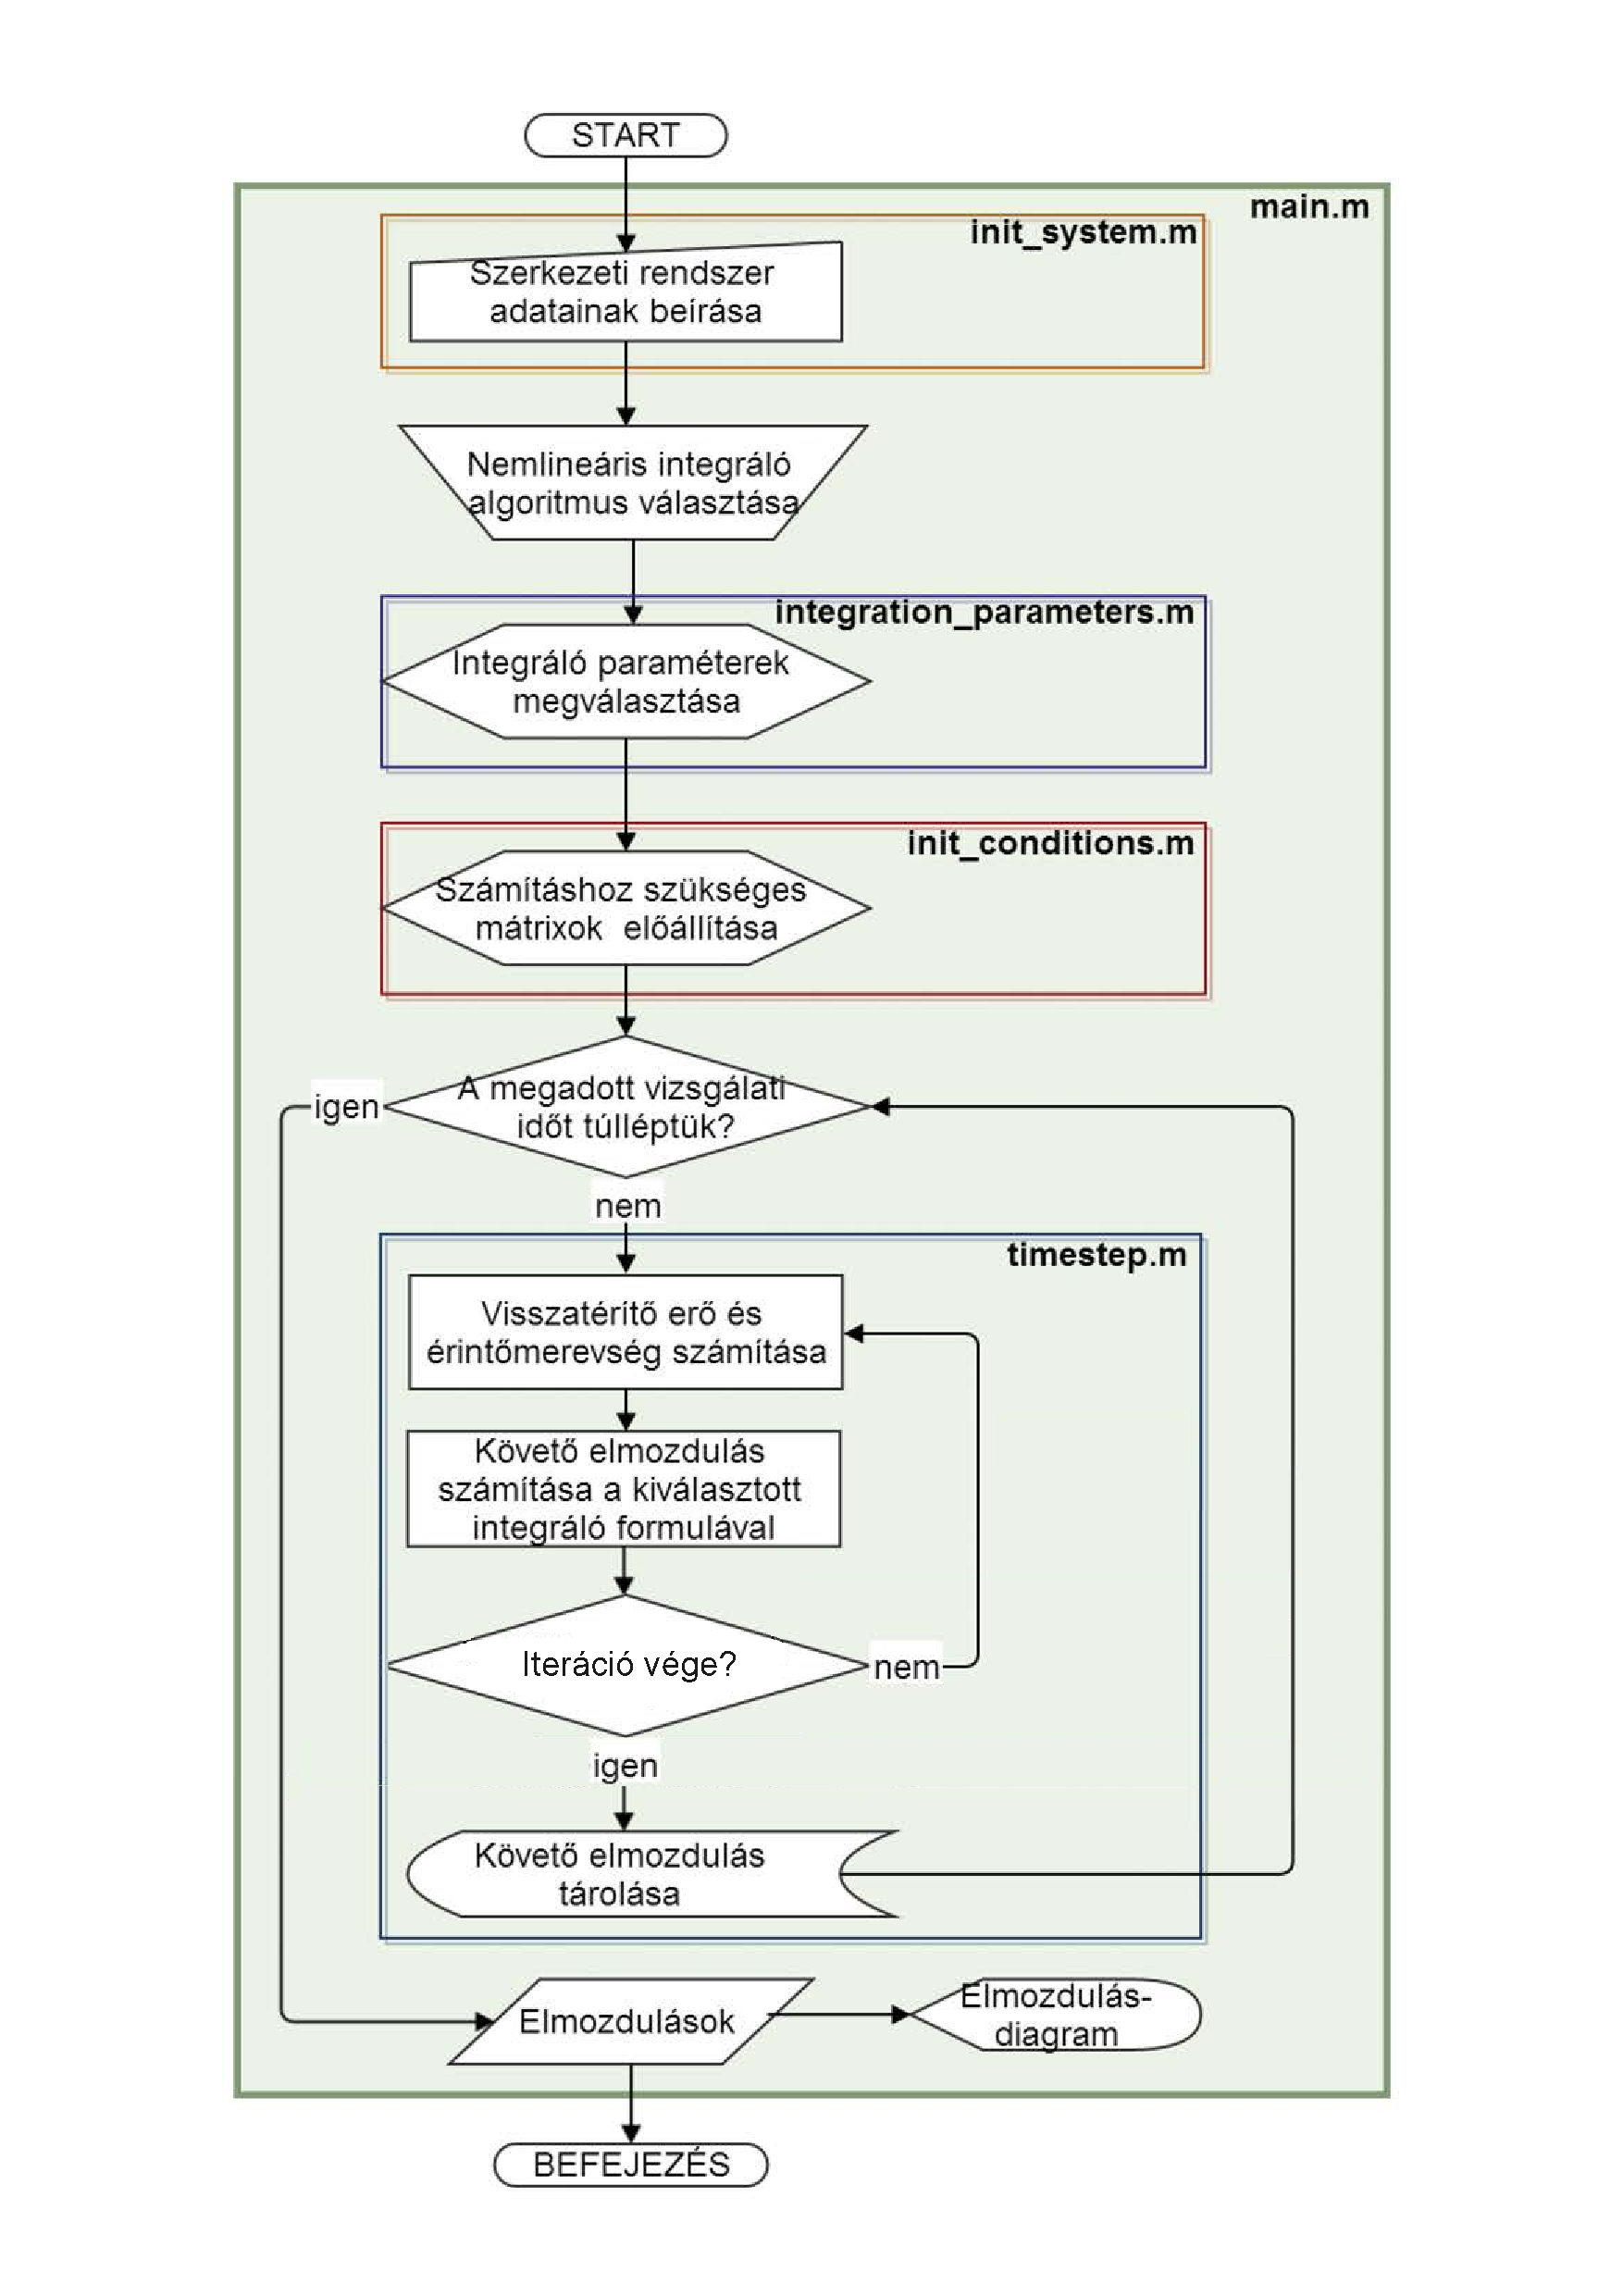
\includegraphics[ width=\textwidth]{nemlinearis_folyamatabra.pdf}
\caption{A nemlineáris időlépéses megoldó program folyamatábrája.}
\label{fig:nemlinprog}
\end{figure}

A nemlineáris megoldó program szintén műveleti blokkokból áll, ezek közül néhány blokk feladata összeegyeztethető a lineáris programnál a \ref{subsec: lin prog szerk} pontban bemutatott szkriptekével. A teljes programkód a Függelék \ref{chap: függ nemlinprog}. pontjában található. A  műveleti parancssort és az inicializáló és számító blokkokat a \verb|main.m| fájl tartalmazza. Indításkor egy biztonsági törlés elvégzése után meghívja az \verb|init_system.m| szkriptet a szerkezet adatainak beolvasására. Ezt követi a felugró menü, amiben a használandó nemlineáris integráló algoritmust választhatjuk ki. A main az egyik Newmark eljárás választása esetén futtatja  az integráló paraméterek és az iterációk adatainak inicializálására az \verb|integration_parameters.m| szkriptet az integráló paraméterek és az iterációk adatainak inicializálására, majd hívja az \verb|init_conditions.m| fájlt a kiválasztott algoritmushoz tartozó helyfoglaló és  előre definiálható segédmátrixok előállítására. Ezt az időlépésekhez tartozó for ciklus követi. A ciklusban a \verb|timestep.m| szkript számolja az időlépésenkénti érintőmerevséget, és (Newmark eljárásoknál kvázi-Newton-Raphson iterációt alkalmazva) a visszatérítő erőt is, valamint ezek segítségével a következő időpontbeli elmozdulást. Végül a main kirajzolja az eredményeket egy elmozdulás-idő diagramon.

 A vizsgált szerkezet adatai az \verb|init_system.m| fájlban találhatók. Ezek a vizsgálat időtartama, a diszkrét időpillanatok lépésköze, a szerkezetet leíró tömeg-, merevségi és csillapítási mátrixok, a tehervektor,  az $\mathbf{u}_0$ és  $\mathbf{\dot{u}}_0$  kezdeti feltételek, valamint a visszatérítő erő és az érintőmerevség számításokhoz szükséges kezdeti értékek és globális változók. Ha az adott feladatban szükséges, szintén itt számítjuk a szerkezet sajátkörfrekvenciáit és sajátrezgésalakjait.
 
 A Newmark algoritmusoknál használt integrálási paramétereket, valamint  a kvázi-Newton-Raphson iteráció adatait  az \verb|integration_parameters.m| fájlban lehet beállítani.  Ezek a $\gamma$ és a $\beta$ paraméterek,  az iterációk száma és az iteráció leállásához szükséges  kritérium feltétel. 
 
 Az \verb|init_conditions.m| szkript hozza létre a kiválasztott algoritmushoz tartozó helyfoglaló mátrixokat mint az elmozdulás-, a sebesség- és a gyorsulásvektorok mátrixát, és az  előre definiálható segédmátrixokat. Centrális differenciák módszere esetén elvégzi a hatékony tömegmátrix invertálását.
 
 A \verb|timestep.m| szkriptben az időlépésekhez tartozó számítások parancssora található. A fájl végzi a visszatérítő erő és  az érintőmerevség frissítését. A Newmark formulák esetében kvázi-Newton-Raphson iterációval számítja a következő  időpillanatbeli elmozdulásokat, és az iterációt követően  tárolja  az eredményeket.

A nemlineáris program futásához szükség van a visszatérítő erő és az érintőmerevség időlépésenkénti számítására. A visszatérítő erő számítása a  \verb|resisting_force.m|, az érintőmerevségé pedig a  \verb|tangent_stiffness.m| függvényfájlokkal történik, ezek tartalmazzák  a nemlineáris  viselkedést leíró függvényeket. A nemlineáris anyagmodell módosítása  ebben a két fájlban egyszerűen megoldható. A számításhoz szükséges globális változókat az \verb|init_system.m| szkriptben adjuk meg.

A program használatát bemutatom statikus probléma vizsgálatára, több csillapítási tényező értéket figyelembe véve, majd  alkalmazom a programot dinamikus probléma vizsgálatára különböző terhelések mellett. 
 
\subsection{A program használata statikus  probléma vizsgálatára} \label{subsec:nemlinstat}

Nem írtam külön programot a statikus nemlineáris feladatok vizsgálatára, de a dinamikus vizsgálatra fejlesztett program is használható erre a célra. Ehhez a teherfüggvényt konstans értékűre kell felvenni, és megfelelően nagy csillapítást kell alkalmazni. A feladat a teherszintek nemlineáris hatásának összehasonlítására alkalmazható.

A feladatban a \ref{subsec:lingerj} pontban bemutatott kétszabadságfokú szerkezetet vizsgáljuk, azonban a csillapítás és a teherfüggvény eltérő, és a szintenkénti merevség  nemlineáris. A megfelelően nagy csillapítás bemutatására különböző $\xi$ paramétereket alkalmaztam.
\begin{align*}
\mathbf{q} & = \mathbf{q}_0 \cos{0t} \\
\mathbf{C} & = \alpha\mathbf{M}+\beta\mathbf{K}  &   \xi & = 0,1 ; 0,5 ; 1,1 
\end{align*}

Az anyagi nemlinearitást  egy arkusz tangens függvénnyel vettem figyelembe.  Azért ezt választottam, mert látványosan nemlineáris, de rugalmas modell, és a lineáris modellhez képest nagyon nagy eltérést mutat nagy alakváltozások esetében. Azonban megjegyezném, hogy ez az anyagmodell  fiktív. A visszatérítő erő és az érintőmerevség: 
\begin{align*}
f_s(\Delta{l}) & = a \arctan{b\Delta{l}}, \\
k_T & = \frac{\delta\mathbf{f}_s}{\delta\Delta{l}} = \frac{ab}{1+b^2\Delta{l}^2},
\end{align*}
ahol $a$ és $b$ paramétert úgy választottuk, hogy a kezdeti időpillanatban az érintőmerevség mindkét szinten $k_{T,0} = 18000 \frac{kN}{m}$, azaz a lineáris rendszer merevségével megegyező legyen. 

Az \verb|init_system.m| fájlban a következő eltérések vannak:

\lstinputlisting{"MATLAB/nonlinear_system_322/init_system.m"}

A \verb|resisting_force.m| és a \verb|tangent_stiffness.m| függvények a következők:

\lstinputlisting{"MATLAB/nonlinear_system_322/resisting_force.m"}
\lstinputlisting{"MATLAB/nonlinear_system_322/tangent_stiffness.m"}



\begin{figure}[h!]
\centering
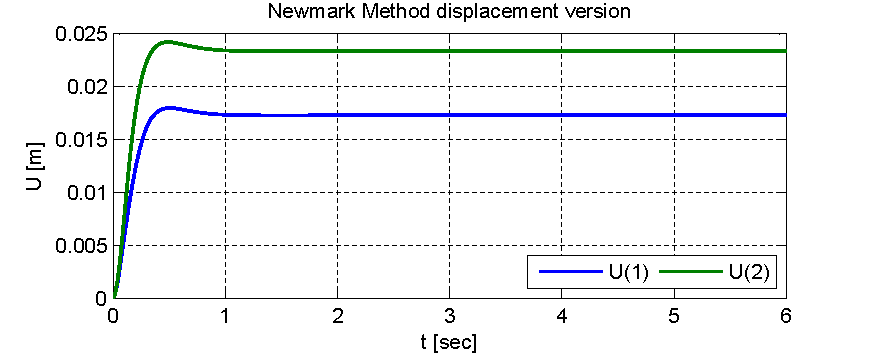
\includegraphics[width=\textwidth]{322_newmark_disp_kszi_0_5.pdf}
\caption{A \ref{subsec:nemlinstat} statikus probléma elmozdulásai a Newmark módszer elmozdulásos változatával, $\xi = 0,5$  esetén.}
\label{fig:322_newmark_disp_0_5}
\end{figure}

A feladat megoldása a Newmark módszer elmozdulásos változatával a \ref{fig:322_newmark_disp_0_5} elmozdulás - idő grafikonon látható. A csillapítás értéke $\xi = 0,5$-del van figyelembe véve. Ez kellően nagy csillapításnak számít, ekkora  mellett már gyorsan lecsillapodik a rezgés. Az eredményeket a \ref{subsec: nemlin eredmény stat} pontban elemzem. A többi csillapításértékkel számított elmozdulások grafikonjai is ebben a  pontban láthatók. 


\subsection{A program használata dinamikus probléma vizsgálatára} \label{subsec:nemlindin}

Ebben a feladatban a dinamikus nemlineáris viselkedést szeretném bemutatni. A  példában szintén a \ref{subsec:lingerj} pontban bemutatott kétszabadságfokú szerkezetet vizsgáljuk. Az anyagmodell megegyezik a \ref{subsec:nemlinstat} statikus problémánál ismertetettel. A szerkezetet különböző amplitúdójú szinuszos terhelésre vizsgáljuk, és összehasonlítjuk az elmozdulásait a terhek függvényében. Az amplitúdók rendre 10, 20, 40 és 80kN. A csillapítás $\xi = 0,05$ paraméterrel van figyelembe véve. 
 
\begin{align*}
\mathbf{q} & = \left[\begin{array}{cc}\mathbf{q}_0\\ \mathbf{q}_0 \end{array}\right] \sin{20t} & \mathbf{q}_0 & = 10; 20; 40; 80 kN\\
\mathbf{C} & = \alpha\mathbf{M}+\beta\mathbf{K}  &   \xi & = 0,05 
\end{align*}

% \lstinputlisting{"MATLAB/nonlinear_system_323/init_system.m"}
% \lstinputlisting{"MATLAB/nonlinear_system_323/resisting_force.m"}
% \lstinputlisting{"MATLAB/nonlinear_system_323/tangent_stiffness.m"}

\begin{figure}[h!]
\centering
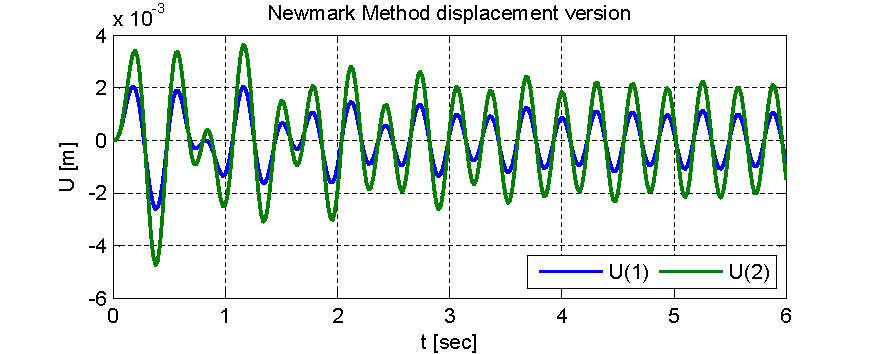
\includegraphics[width=\textwidth]{323_Newmark_disp.pdf}
\caption{A \ref{subsec:nemlindin} dinamikus probléma elmozdulásai a Newmark módszer elmozdulásos változatával, $\mathbf{q}_0 = 20$ esetén.}
\label{fig:323_newmark_disp}
\end{figure}

A \ref{fig:323_newmark_disp} ábrán az elmozdulás - idő diagram látható a Newmark módszer elmozdulásos változatával számolva, $\mathbf{q}_0 = 20$ amplitúdójú teherrel. A program kirajzolja a különböző terhelésekkel számolt elmozdulásokat egy ábrára is, így megfigyelhető, milyen összefüggés van a terhelés és az elmozdulás amplitúdója között. Az eredményeket a \ref{subsec: nemlin eredmény din} pontban mutatom be. 


\section{Az időlépéses módszerek összehasonlítása a programok eredményei alapján}\label{sec: msz összehasonlítás}

\subsection{A lineáris időlépéses megoldó program eredményei gerjesztett rezgés esetén}\label{subsec: lin eredmény gerj}

{\ }

A \ref{subsec:lingerj} gerjesztéses feladat alapján összehasonlíthatók az egyes időlépéses módszerek. Az eredmények a Függelék \ref{sec:függ_lingerj} pontban találhatók. 

Az Euler - módszer ábráján az látszik, hogy a megoldás instabillá vált, az elmozdulások a végtelenbe tartanak. A többi grafikon nagyjából hasonló eredményt mutat, nincs másik kirívó eset.

A dinamikus hatás szemléltetésére kirajzoltattam az elmozdulást az $\mathbf{u}_{st}(t) = \mathbf{K}_0^{-1}\mathbf{q}(t)$ statikus elmozdulással együtt az idő függvényében (\ref{fig:lingerjeredm_newmark_Ku} ábra). Az ábrán jól látható, hogy a szerkezet a terheléssel ellentétes fázisban rezeg, hiszen $\omega > \omega_{01}$, és főleg az első alak van gerjesztve a teherfüggvénnyel.

\begin{figure}[H]
\centering
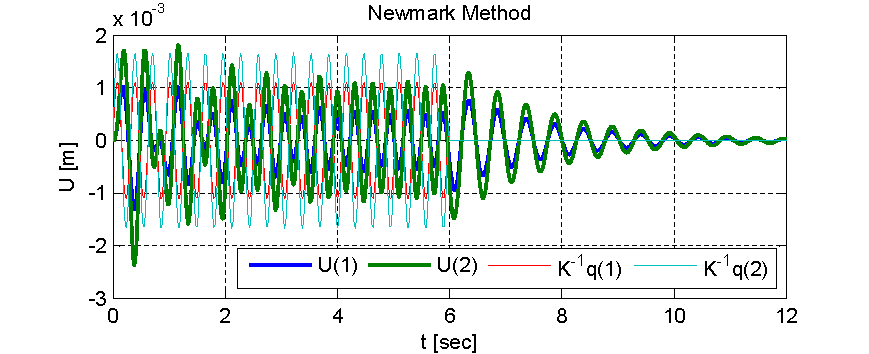
\includegraphics[width=\textwidth]{312_Newmark_Ku.pdf}
\caption{A \ref{subsec:lingerj} gerjesztett rezgéses példa elmozdulásai Newmark módszerrel és a statikus elmozdulás.}
\label{fig:lingerjeredm_newmark_Ku}
\end{figure}



\subsection{A lineáris időlépéses megoldó program eredményei csillapítatlan szabadrezgés esetén}\label{subsec: lin eredmény szabrezg}

{\ }

 A \ref{subsec:szabrezg} szabadrezgéses feladat alapján vizsgálható az egyes időlépéses módszerek stabilitása és pontossága. A \ref {fig:szabrezg_erek_newmark-a} ábrán a rendszer mechanikai energiája, a \ref{fig:szabrezg_erek_newmark-b} grafikonon pedig a fázistérben ábrázolt elmozdulásai láthatók. Az program által kirajzolt  eredmények  a többi módszerrel a Függelék \ref{sec:függ_szabrezg}.  pontjában találhatók. 
 
 A feladatban vizsgálhatjuk az elmozdulást az idő függvényében, és  következtethetünk a periódusidők meghosszabbodására. Azonban a diagramon az amplitúdó változások kicsik,  és a maximumok pontos értéke nehezen érzékelhető, ezért   nehéz ezeket  leolvasni.  A probléma megoldására kirajzoltattam  a mechanikai energiát diszkrét $t_i$ időpontokban, valamint a szabadságfokok elmozdulásának arányát. A mechanikai energiának ekkor nem szabad növekednie stabil rendszereknél, az elmozdulások arányának pedig a fázistér vetületében egyenesnek kell lennie.  
 
A szerkezet mechanikai energiáját a következő képlettel számíthatjuk:
\[ E_m = \frac{1}{2}\mathbf{u}_i^T\mathbf{K}\mathbf{u}_i+\frac{1}{2}\mathbf{u}_i^T\mathbf{M}\mathbf{u}_i\]
Ennek számítását a programkódban a  \verb|main.m| fájlban a következőképp deklaráltam:

  \mcode{ME(:,i) = 1/2*(U(:,i).'*K*U(:,i))+1/2*(dU(:,i).'*M*dU(:,i));}.
  

\begin{figure}[h!b]%
\centering
\subfigure[][]{%
\label{fig:szabrezg_erek_newmark-a}%
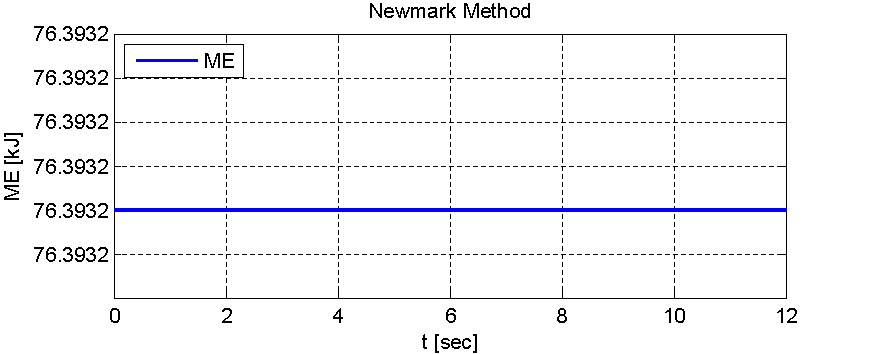
\includegraphics[width=\textwidth]{313_Newmark_mechen.pdf}}%
\\
\subfigure[][]{%
\label{fig:szabrezg_erek_newmark-b}%
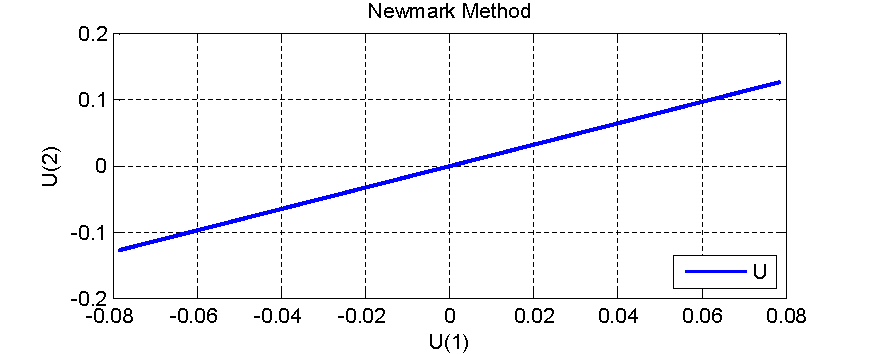
\includegraphics[width=\textwidth]{313_Newmark_elm.pdf}}%
\caption[A \ref{subsec:szabrezg} szabadrezgéses példa megoldásai Newmark módszerrel.]{A \ref{subsec:szabrezg} szabadrezgéses példa megoldásai  Newmark módszerrel:
\subref{fig:szabrezg_erek_newmark-a} a rendszer mechanikai energiája;
\subref{fig:szabrezg_erek_newmark-b} az elmozdulások fázistérben ábrázolva.}%
\label{fig:szabrezg_erek_newmark}
\end{figure}


 A grafikonokat elemezve láthatjuk, hogy az Euler-módszerrel az elmozdulások számítása elszáll, a rendszer mechanikai energiája minden határon túl nő, és az elmozdulások egymáshoz viszonyított előjele is hibás. A Runge-Kutta módszernél a csillapítás negatív előjelű a mechanikai energia növekszik, a Wilson-$\theta$ és HHT-$\alpha$ módszereknél pedig pozitív előjelű csillapítás érzékelhető. A periódusidő meghosszabbodása a Wilson-$\theta$ eljárásnál a legkisebb, és  Newmark,  HHT-$\alpha$, valamint CR algoritmusokkal számolva ehhez képest csak minimálisan növekszik. A legnagyobb meghosszabbodás a Runge-Kutta módszernél keletkezik.
 





\subsection{A nemlineáris időlépéses megoldó program eredményei statikus  probléma esetén}\label{subsec: nemlin eredmény stat}


A \ref{subsec:nemlinstat} statikus nemlineáris feladatban bemutatom, hogy a különböző $\xi$ értékek milyen mértékben befolyásolják az elmozdulások kialakulását. A \ref{fig:322_newmark_disp} ábrán az elmozdulás - idő függvények láthatók $\xi = 0.1, 0.5,$ és $1.1$ értékekre, a Newmark módszer elmozdulásos változatával számolva. A $\xi = 0.1$ értéknél (\ref{fig:322_newmark_disp-a} ábra) kialakul egy gyorsan lecsengő rezgés az állandósult érték körül. A $\xi = 0.5$ paraméter esetében (\ref{fig:322_newmark_disp-b} ábra) még kialakul rezgés (hiszen túlmegy a statikus helyzeten), de nagyon gyorsan lecseng. A $\xi = 1.1 > 1$ esetén (\ref{fig:322_newmark_disp-c} ábra) már nagy csillapításról beszélünk, ekkor nem alakul ki rezgés, és az elmozdulás értéke nem éri el az állandósult értéket.

A végső elmozdulás az első szinten $17 mm$, a második szinten pedig $23 mm$.  Az eredmények alapján a csillapítási tényezőre a  $\xi = 0,5$ értéket javaslom használni.

Az egyes módszerekkel számolt megoldások grafikonjait a Függelék \ref{sec:függ 322} pontja tartalmazza.


\begin{figure}%
\centering
\subfigure[][]{%
\label{fig:322_newmark_disp-a}%
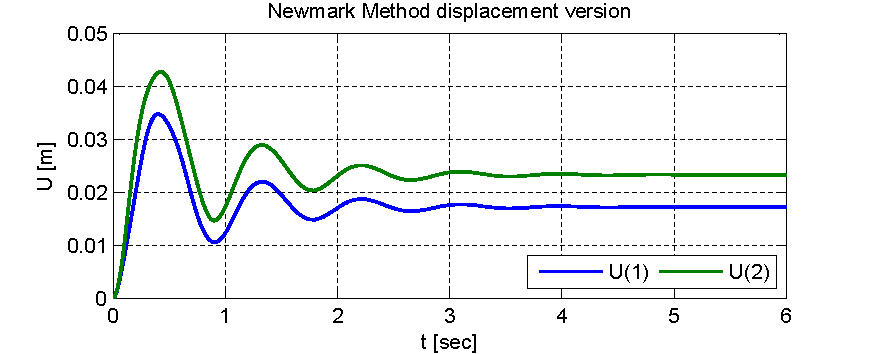
\includegraphics[width=0.75\textwidth]{322_newmark_disp_kszi_0_1.pdf}}%
\\
\subfigure[][]{%
\label{fig:322_newmark_disp-b}%
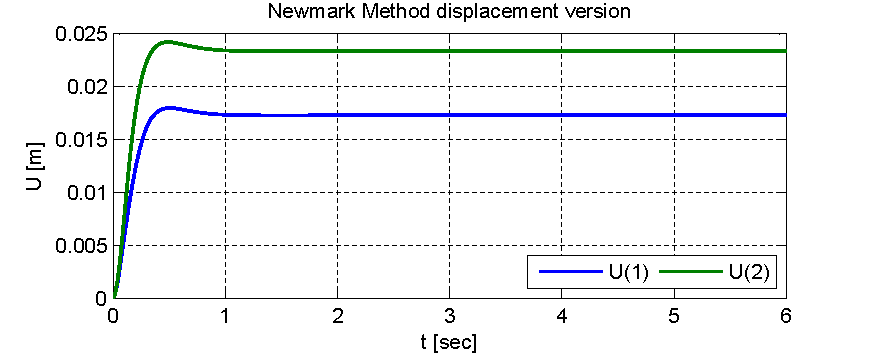
\includegraphics[width=0.75\textwidth]{322_newmark_disp_kszi_0_5.pdf}}%
\\
\subfigure[][]{%
\label{fig:322_newmark_disp-c}%
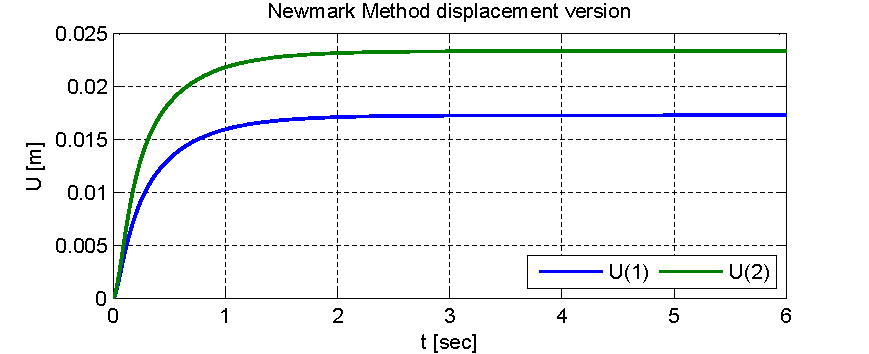
\includegraphics[width=0.75\textwidth]{322_newmark_disp_kszi_1_1.pdf}}%
\caption[A \ref{subsec:nemlinstat} statikus probléma elmozdulásai a Newmark módszer elmozdulásos változatával.]{A \ref{subsec:nemlinstat} statikus probléma elmozdulásai a Newmark módszer elmozdulásos változatával:
\subref{fig:322_newmark_disp-a} $\xi = 0.1$;
\subref{fig:322_newmark_disp-b} $\xi = 0.5$; 
\subref{fig:322_newmark_disp-c}  $\xi = 1.1$.}%
\label{fig:322_newmark_disp}%
\end{figure}
 


\subsection{A nemlineáris időlépéses megoldó program eredményei dinamikus probléma esetén}\label{subsec: nemlin eredmény din}

{\ }

A \ref{subsec:nemlindin} dinamikus nemlineáris feladat kapcsán  megfigyelhetjük a nemlineáris viselkedést. Most különböző terhelés hatására vizsgáljuk az elmozdulásokat. A tapasztalat szerint a teherfüggvényben az $\omega$  értéke meghatározza az időbeli lefutást.

A \ref{fig:323_newmark_disp_q_var_1} ábrán az elmozdulások láthatók az idő függvényében, különböző terhelések hatására a Newmark módszer elmozdulásos változatával számítva.  A grafikonról leolvasható, hogy a válasz a periodikus alakot megtalálja, viszont a maximum elmozdulás értékek nem a terhek arányát tükrözik. Az egyes módszerekkel számolt megoldások grafikonjait a Függelék \ref{sec:függ 323} pontja tartalmazza. 



\begin{figure}[h!p]
\centering
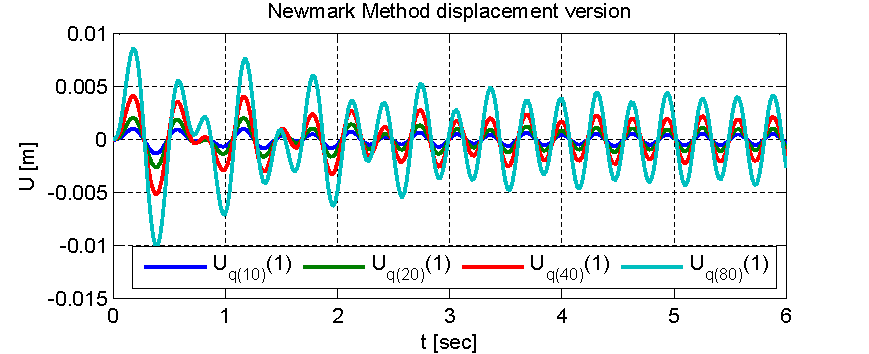
\includegraphics[width=0.75\textwidth]{323_Newmark_disp_q_var.pdf}
\caption{A \ref{subsec:nemlindin} dinamikus probléma megoldásai az első csomópontra a Newmark módszer elmozdulásos változatával különböző terhelésekre.}
\label{fig:323_newmark_disp_q_var_1}
\end{figure}


\chapter[Időlépéses program verifikálása]{Időlépéses módszereket alkalmazó program verifikálása}\label{chap: lin+nemlin verif.}

{\ }

A következőkben a \ref{chap: lin+nemlin progi}. fejezetben ismertetett lineáris  és a nemlineáris megoldó programok verifikálását végzem el szakirodalmi példákkal. A példák mindkét program esetében  Chopra könyvében \cite{chopra}  találhatók. A lineáris megoldó programban a 16.1 példát, a nemlineáris megoldóban pedig a 16.4 feladatot számoltam.


\section{A lineáris időlépéses megoldó program verifikálása gerjesztett rezgésre}\label{sec:linver}

{\ } 

A lineáris megoldó program verifikálását Chopra könyvének \cite{chopra} 16.1 példája alapján végeztem.   A könyvben az angolszász mértékegységek használatosak, így a verifikálás során a könnyebb átláthatóság érdekében én is ezeket használtam. A nehézségi gyorsulást mindenhol $386 in./sec^2$ értékkel számoltam. A feladatban egy ötszintes épületet vetünk alá egy teljes periódus szinuszos talajgyorsulásnak, és ennek vizsgáljuk a válaszát Newmark módszerrel, lineáris gyorsulást feltételezve. A  gyorsulást az $\mathbf{\ddot{u}}_{g,0}\sin{2\pi{t}}$ függvény írja le, az amplitúdója  $\mathbf{\ddot{u}}_{g,0} = 0.5 g$ , periódusideje 1 sec. A támaszrezgéshez tartozó teher ez alapján számítható. Az egyes szintek tömege 100 kips/g, a szintenkénti merevség pedig 100 kips/in.; a csillapítási tényező minden módban 5\%. A feladatban a klasszikus modális csillapítással számolunk. A vizsgálat 2 sec-ig tart, az időlépések nagysága 0.1 sec. A szerkezet geometriája a \ref{fig:ex3-a} ábrán, a talajgyorsulások függvénye pedig a \ref{fig:ex3-a} grafikonon látható.



\begin{figure}%
\centering
\subfigure[][]{%
\label{fig:41-a}%
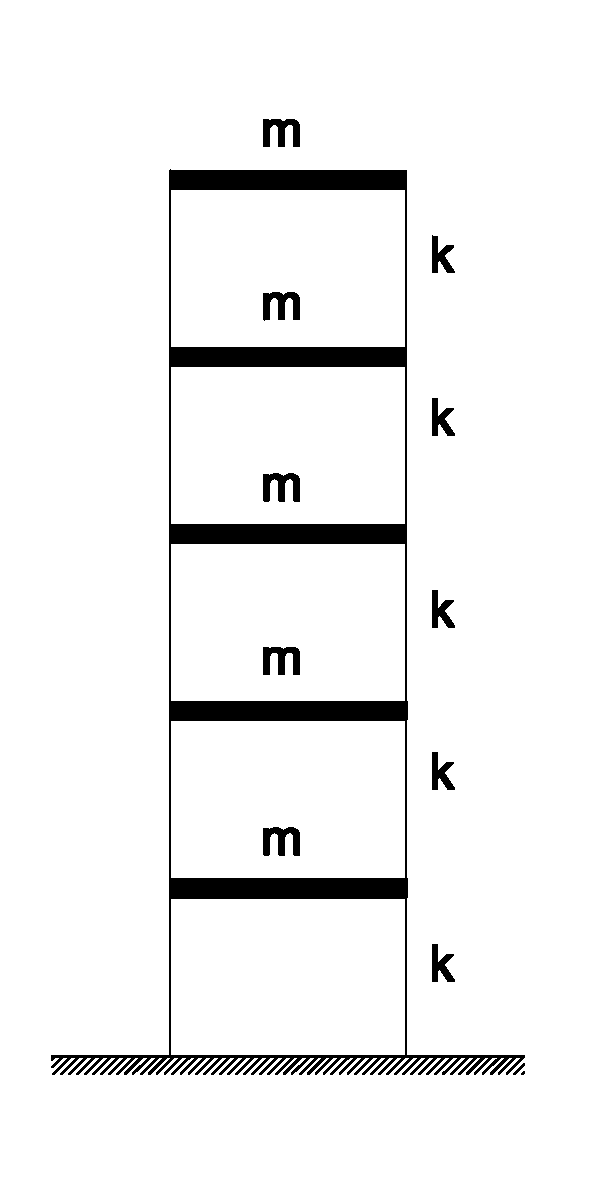
\includegraphics[width=0.25\textwidth]{otszintes_keret.pdf}}%
\hspace{8pt}%
\subfigure[][]{%
\label{fig:41-b}%
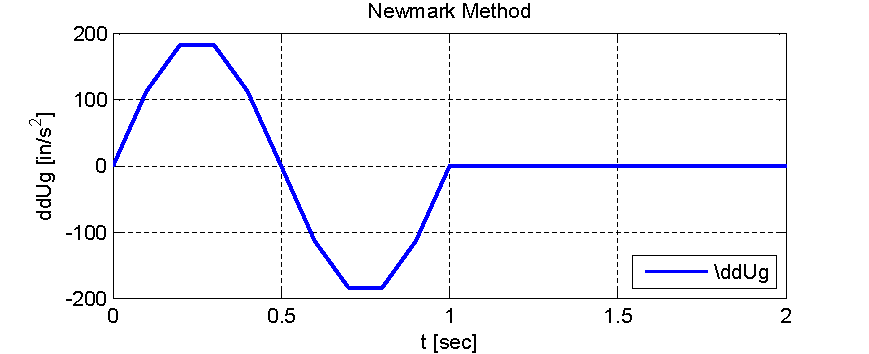
\includegraphics[width=0.7\textwidth]{41_ddUg.pdf}}%
\caption[A \cite{chopra} 16.1 feladatban vizsgált ötszintes keret és a  talajgyorsulás.]{\subref{fig:41-a} A \cite{chopra} 16.1 feladatban vizsgált ötszintes keret és \subref{fig:41-b}  a  talajgyorsulás}
 \label{fig:41}%
\end{figure}

A szerkezet analíziséhez modálanalízist és direkt integrálást együttesen alkalmaztunk. A számításhoz csak az első két módot használtuk, a többit elhanyagoltuk, így a rendszert kétszabadságfokúra redukáltuk. 

A rendszert leíró mátrixok a következők:
\begin{align*}
  & t_{max}  = 2 sec  & & \Delta{t} = 0,1 sec   & \\
  & \mathbf{M}  = 100\left[\begin{array}{rrrrr}  1 & 0 & 0 & 0 & 0  \\ 0 & 1 & 0 & 0 & 0 \\ 0 & 0 & 1 & 0 & 0 \\ 0 & 0 & 0 & 1 & 0 \\ 0 & 0 & 0 & 0 & 1  \end{array} \right] \frac{kips}{g}   &  & \mathbf{K} = 100 \left[\begin{array}{rrrrr} 2 & -1 & 0 & 0 & 0  \\ -1 & 2 & -1 & 0 & 0 \\ 0 & -1 &2 & -1 & 0 \\ 0 & 0 & -1 & 2 & -1 \\ 0 & 0 & 0 & -1 & 1 \end{array} \right]\frac{kips}{in.}  &  \\
  & \mathbf{C}_n  = \xi_n(2\mathbf{M}_n\omega_n)  &  & \xi = 0,05  & \\
  & \mathbf{q}_1  = -100\left[\begin{array}{c} 1 \\ 1 \\ 1 \\ 1 \\ 1 \end{array} \right]\mathbf{\ddot{u}}_{g}(t) & & \mathbf{\ddot{u}}_{g}(t) = \mathbf{\ddot{u}}_{g,0}\sin{2\pi{t}}  &  \\
  & \mathbf{u}(0)  = \left[\begin{array}{c} 0 \\ 0 \\ 0 \\ 0 \\ 0  \end{array} \right]  & & \mathbf{\dot{u}}(0) = \left[\begin{array}{c} 0 \\ 0 \\ 0 \\ 0 \\ 0 \end{array} \right] & 
  \end{align*}

A számítást Newmark módszerrel, lineáris gyorsulás feltételezésével végeztem. A módszerhez tartozó paraméterek értékei: $\gamma = \frac{1}{2}$ és $\beta = \frac{1}{6}$.

A szerkezetet bemeneti adatai az \verb|init_system.m| fájlban:
\lstinputlisting{"MATLAB/linear_system_41/init_system.m"}


A számított elmozdulások grafikonjai a \ref{fig:ex3} ábrán láthatók. A számítás az első modális szinten pontosnak tekinthető, mivel a lépésközök nagysága $\Delta{t} = 0,01 sec$, a sajátperiódusidő pedig $T_1 = 2\pi/5,592 = 1,12 sec$, tehát a lépésköz kisebb a természetes periódus tizedénél, teljesül az ökölszabály. Ugyanakkor a második modális szinten $\Delta{t}/T_2 = 0,16$ - ra adódik, ami nem felel meg a kritériumnak, ezért a második szint eredményei kevésbé pontosak. Ez a különbség megfigyelhető a  \ref{fig:ex3-a} és   \ref{fig:ex3-b} grafikonokon is. A modális elmozdulás görbéje az első szinten folytonosnak látszik, viszont a második szint modális elmozdulása inkább törött vonallal ábrázolható. 
 
\begin{figure}[h!b]%
\centering
\subfigure[][]{%
\label{fig:ex3-a}%
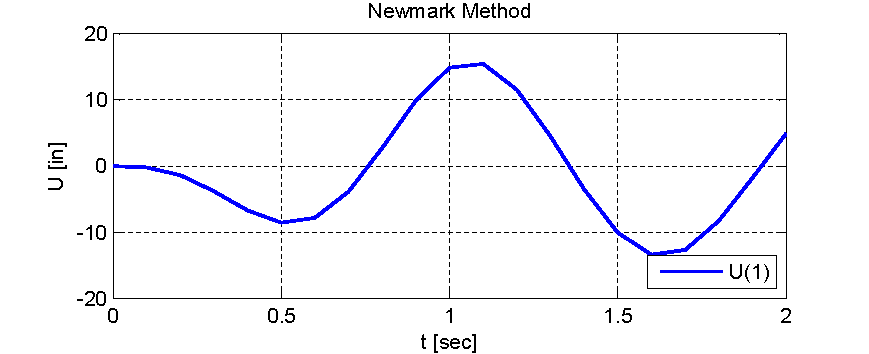
\includegraphics[width=0.75\textwidth]{41_U_1.pdf}}%
\\
\subfigure[][]{%
\label{fig:ex3-b}%
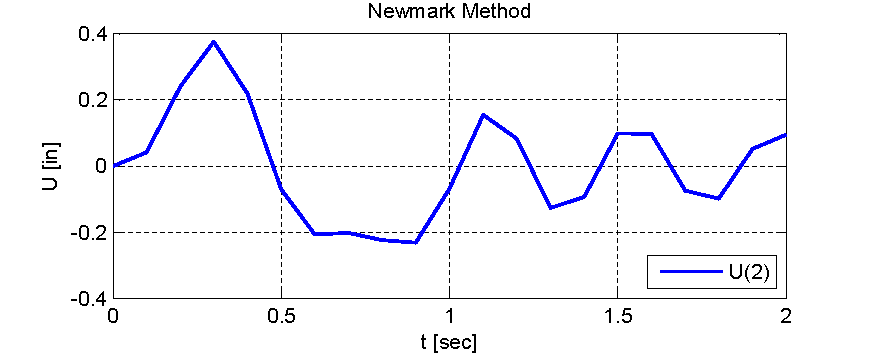
\includegraphics[width=0.75\textwidth]{41_U_2.pdf}}%
\\
\subfigure[][]{%
\label{fig:ex3-c}%
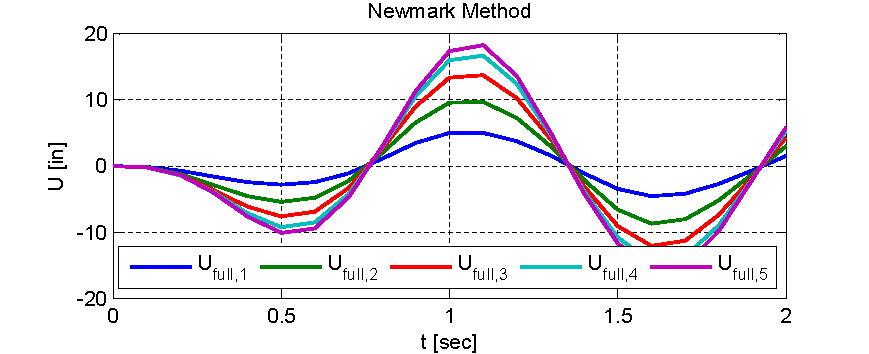
\includegraphics[width=0.75\textwidth]{41_U_full.pdf}}%
\caption[A \cite{chopra} 16.1 feladat eredményei a lineáris megoldó programmal.]{A \cite{chopra} 16.1 feladat eredményei a lineáris megoldó programmal:
\subref{fig:ex3-a} és \subref{fig:ex3-b}  modális elmozdulások;
\subref{fig:ex3-c} elmozdulások.}%
\label{fig:ex3}%
\end{figure}

A lineáris megoldó program számításainak eredményei négy tizedesjegy pontosan megegyeznek a könyvben közzétett eredményekkel. A számítás eredményei a \ref{161_table saját}, a könyvben ismertetett eredmények pedig a \ref{161_table} táblázatokban olvashatók. A \ref{161_table} referencia eredmények táblázatában a harmadik oszlop, ami modális elmozdulások  értékeit tartalmazza második szinten, feltehetőleg hibásan lett beírva, mivel ez megegyezik az első szint modális elmozdulásait mutató második oszloppal. Ettől a nyomdai hibától eltekintve a két táblázat megegyezik. A lineáris megoldó program verifikálása sikeresnek tekinthető.

\begin{table}[p]
\centering
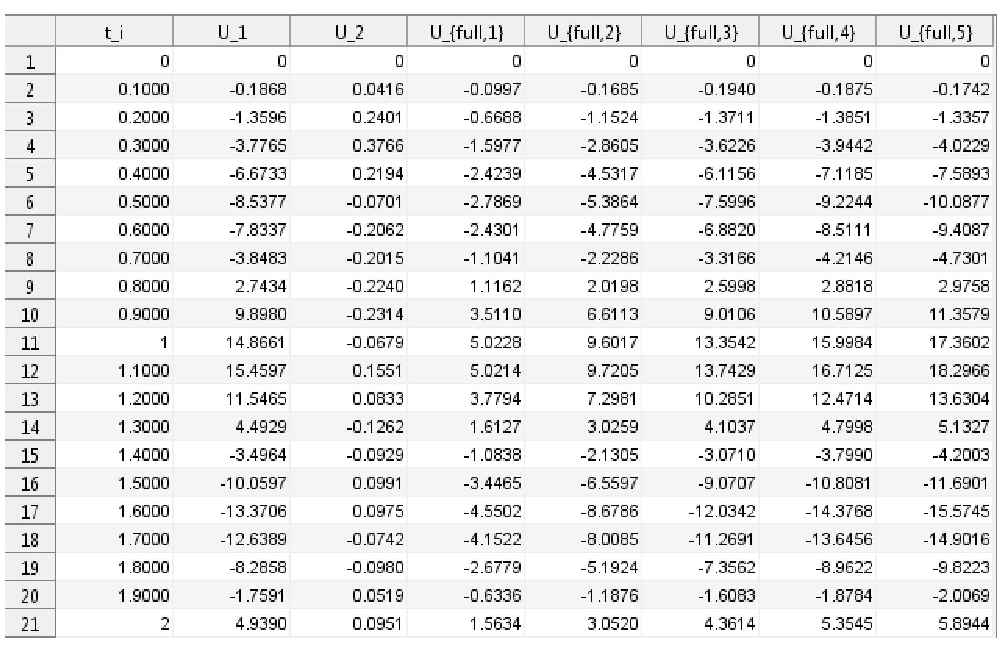
\includegraphics[width=\textwidth]{41_table.pdf}
\caption{A \cite{chopra} 16.1 példa megoldásai a lineáris megoldó programmal.}
\label{161_table saját}
\end{table}

\begin{table}[p]
\centering
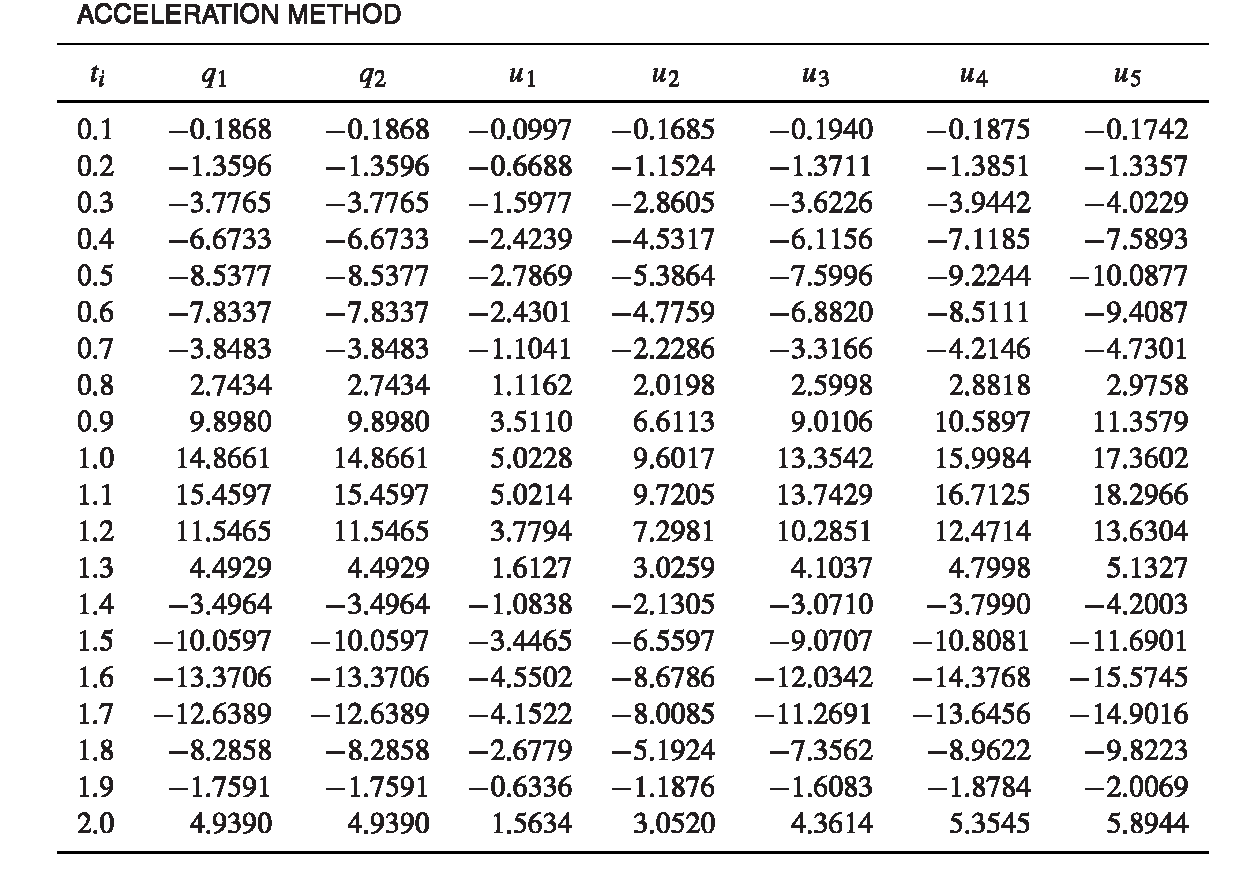
\includegraphics[trim = 0mm 0mm 0mm 7mm, clip, width=\textwidth]{41_chopra_table.pdf}
\caption{A \cite{chopra} 16.1 példa referencia  megoldásai.}
\label{161_table}
\end{table}




\newpage
\section{A nemlineáris időlépéses megoldó program verifikálása dinamikus problémára}

{\ }

A nemlineáris megoldó programot  Chopra könyvének \cite{chopra} 16.4 példája alapján verifikáltam.  Ebben a feladatban is az angolszász mértékegységekkel dolgoztam. A feladat szerint a könyv 16.1 példájából ismert  ötszintes keretet vizsgáljuk (\ref{fig:41-a} ábra), amire ugyanaz az 1 sec periódusidejű teljes szinuszhullám talajgyorsulás hat. A gyorsulás grafikonja a \ref{fig:41-b} ábrán látható. A mozgásegyenlet megoldását ezúttal a  konstans átlagos gyorsulást feltételező nemlineáris Newmark módszerrel oldottuk meg, az egyes időlépésekben kvázi-Newton-Raphson iterációval közelítve a megoldást. Az integrálási paraméterek értékei: $\gamma = \frac{1}{2}$ és $\beta = \frac{1}{4}$. 

A szerkezet anyagmodellje ezúttal a könyv 16.2 példájában alkalmazott  bilineáris  anyagmodell, $k = 100 kips/in.$ kezdeti merevséggel és $\alpha = 0.05$ utólagos merevség csökkenéssel. A határnyíróerő $V_{jy} = 125 kips$. Az anyagmodell diagramja a \ref{fig:nemlinpassz amodell} ábrán látható. Az anyagmodell ismertetése a könyvben hiányos, nem derül ki, hogy a felkeményedést követő visszaterhelésnél hogyan viselkedik az anyagunk. Az ismert adatok alapján egy lineárisan rugalmas - lineárisan felkeményedő anyagmodellt alkalmaztam.

\begin{figure}[h!]
\centering
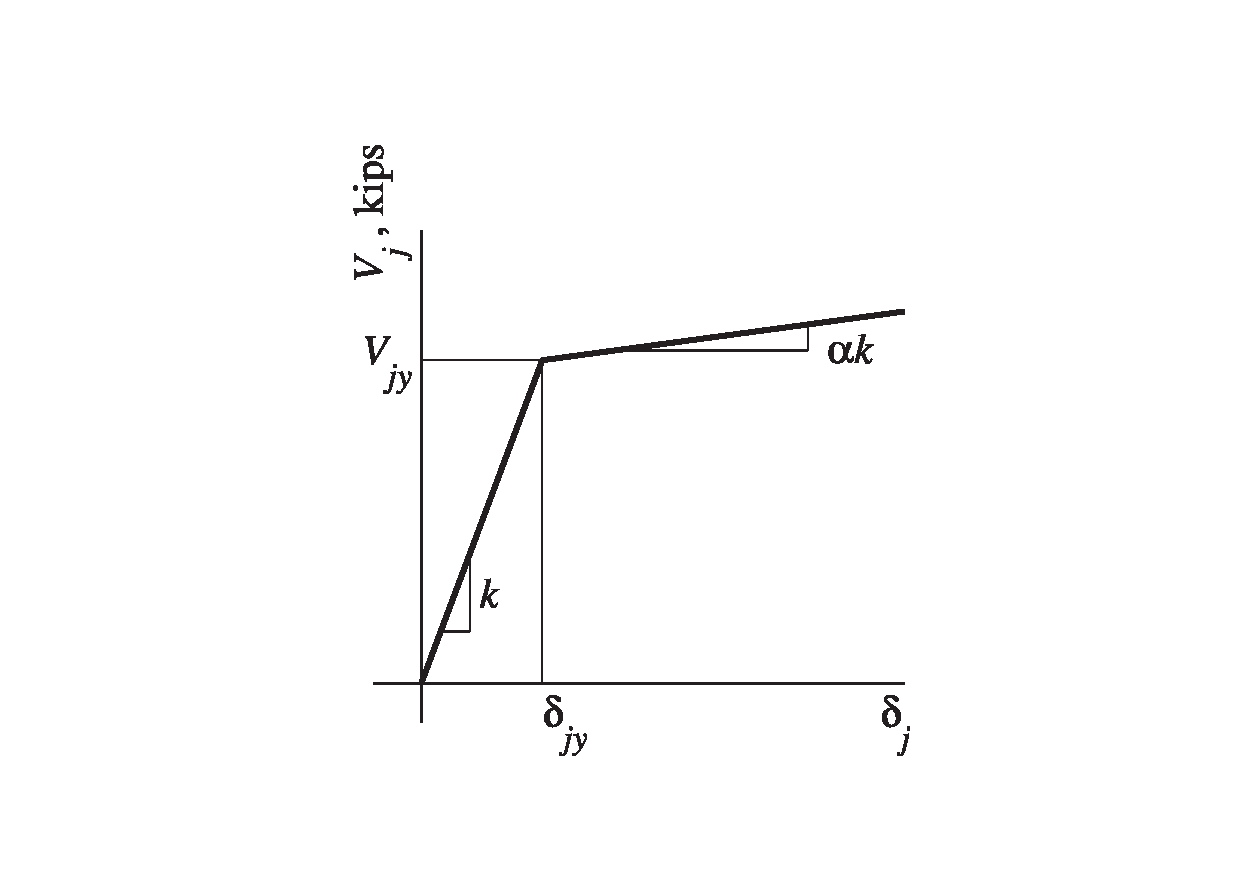
\includegraphics[width=0.75\textwidth]{bilin_amod.pdf}
\caption{A feladatban alkalmazott bilineáris anyagmodell \cite{chopra}}
\label{fig:nemlinpassz amodell}
\end{figure}

 A szerkezet tömeg- és merevségi mátrixát már korábban előállítottuk a \ref{sec:linver} pontban. A vizsgálat időlépése $0.1 sec$, a kezdeti feltételek zérus értékűek,  a csillapítási tényező minden módban 5\%.Ezúttal a teljes szerkezeten futtatjuk  a számításokat. A csillapítási mátrixot a példában  a modális csillapítási mátrixok szuperpozíciójával vettük figyelembe. Ez egy alternatív módszer a modális csillapítási tényezőkből előállított klasszikus csillapítási mátrix számítására. A csillapítási mátrixot a következő összefüggés alapján számítottuk:
\begin{equation*}
     \mathbf{C}  = \mathbf{M}(\sum_{n = 1}^{N}\frac{2\xi_n\omega_n}{M_n}v_nv^t_n)\mathbf{M}     
\end{equation*}

Az \verb|init_system.m| fájlban a szerkezet csillapítási mátrixának számítása és a visszatérítő erő számításához szükséges állandók: 

\lstinputlisting[firstline=44, lastline=58]{"MATLAB/nonlinear_system_42_keplekeny/init_system.m"}
\lstinputlisting[firstline=83, lastline=101]{"MATLAB/nonlinear_system_42_keplekeny/init_system.m"}

A visszatérítő erő és az érintőmerevség számítása a \verb|resisting_force.m| és \verb|tangent_stiffness.m| függvényekben:

\lstinputlisting{"MATLAB/nonlinear_system_42_keplekeny/resisting_force.m"}
\lstinputlisting{"MATLAB/nonlinear_system_42_keplekeny/tangent_stiffness.m"}

A \ref{fig:ize} ábrán az elmozdulások láthatók az idő függvényében. A   16.1 példa \ref{fig:ex3-c} ábrán látható elmozdulásaival összehasonlítva látható, hogy a képlékeny szerkezet ugyanazt  a terhelést a képlékenyedés megjelenését követően lassabban követi a lineáris szerkezetnél, viszont a maximális elmozdulások a képlékeny szerkezet esetében kisebbek. 

 
\begin{figure}[h!]
\centering
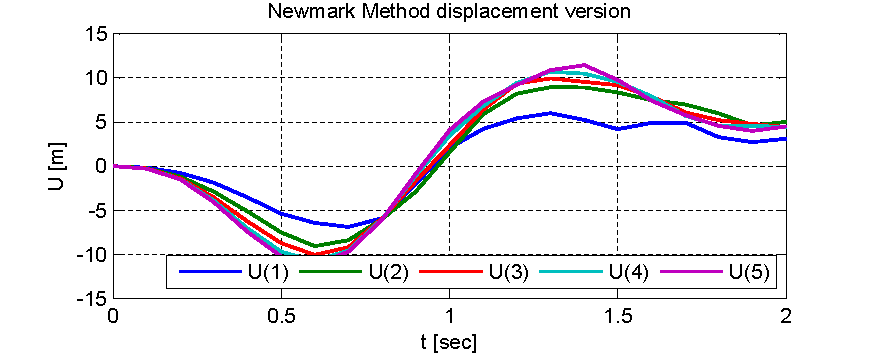
\includegraphics[width=\textwidth]{42_ufull.pdf}
\caption[A \cite{chopra} 16.4 feladat elmozdulásai a nemlineáris megoldó programmal.]{A \cite{chopra} 16.4 feladat elmozdulásai a nemlineáris megoldó programmal.}
\label{fig:ize}
\end{figure}


A \ref{164_table saját} és \ref{164_table} táblázatokban látható, hogy a nemlineáris megoldó programmal számított eredmények az első 6 sorban  négy tizedesjegy pontosan megegyeznek a könyvben ismertetett eredményekkel. Ezt követően azonban eltérések jelentkeznek a két táblázatban. Az első eltérés a 7. időpillanatban van, ez megegyezik a visszaterhelés kezdetével, vagyis  az különbségek a visszaterhelést követő számításokban jelennek meg. Ennek oka  az, hogy a példában az anyagmodell  hiányos leírása miatt  a könyv számításaihoz használt és az általam a nemlineáris programban alkalmazott anyagmodell eltérően veszi figyelembe a képlékenyedés utáni visszaterhelés hatását. Az első szakaszon számított megegyező eredmények miatt, és mert a második szakasz eredményeiben észlelt különbségek okát ismerjük, kijelenthetjük, hogy a nemlineáris megoldó program jól működik, a verifikálás sikeres.

\begin{table}[p]
\centering
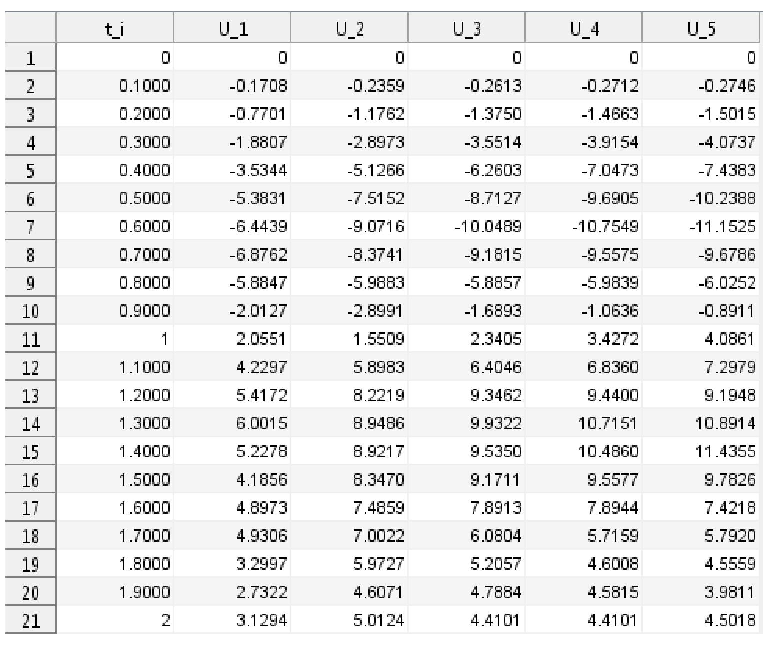
\includegraphics[width=0.8\textwidth]{42_table.pdf}
\caption{A \cite{chopra} 16.4 példa megoldásai a nemlineáris megoldó programmal.}
\label{164_table saját}
\end{table}

\begin{table}[p]
\centering
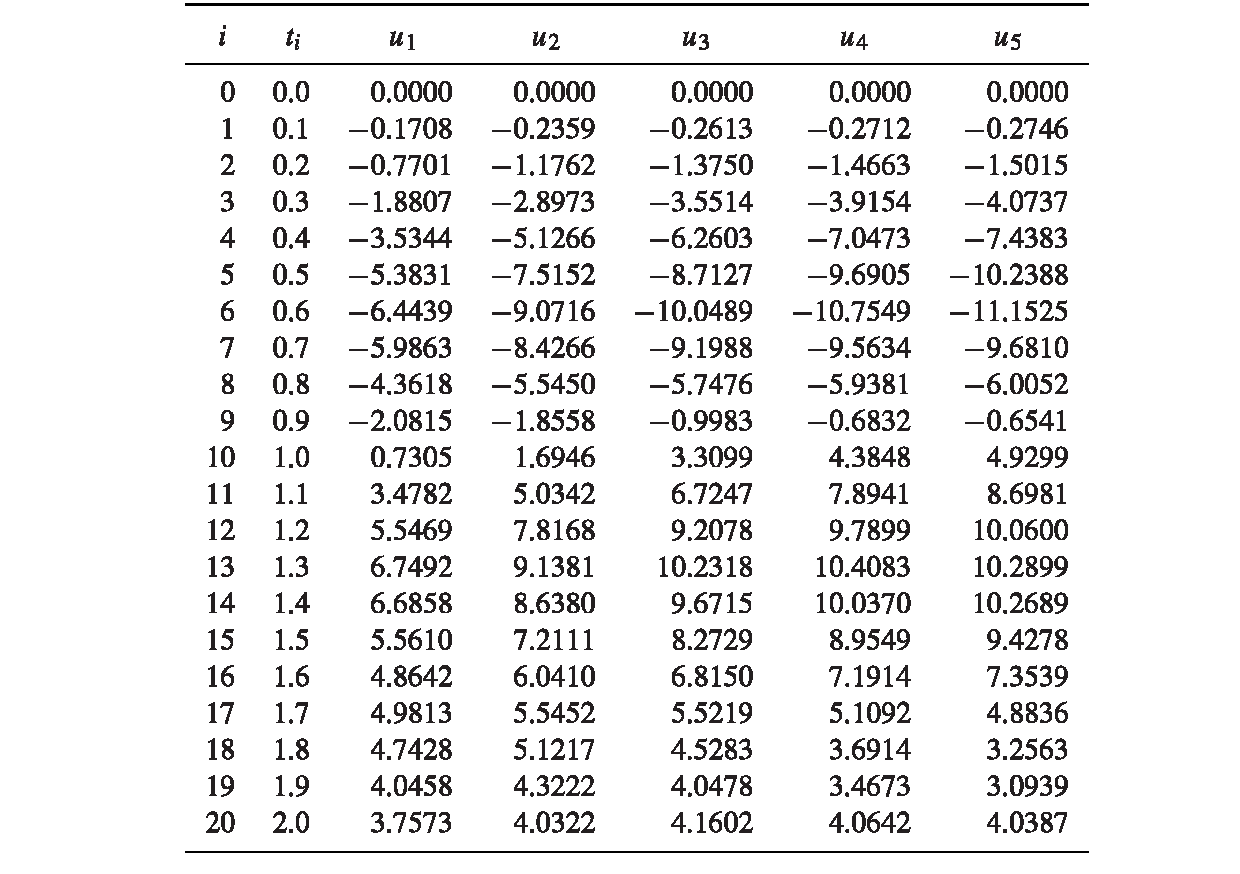
\includegraphics[width=\textwidth]{42_chopra_table.pdf}
\caption{A \cite{chopra} 16.4 példa referencia  megoldásai.}
\label{164_table}
\end{table}



\chapter{Hibrid szimulációs módszer}\label{chap:hibrid}

{\ }


A hibrid szimulációs módszer a numerikus számítások és a kísérleti eljárások előnyeinek ötvözésén alapul.  A módszer alapötlete még a '70-es évekből származik, azonban az irányítástechnikai fejlettség és a számítógépek  kapacitása csak  nagyjából a 2000-es évektől tette lehetővé elterjedését. A fejlődésben nagy előrelépést jelentett a CR algoritmus megjelenése és sikeres alkalmazása a hibrid vizsgálatokra.  Napjainkban az igény is megnőtt rá, mivel a földrengésre vonatkozó tervezési alapelvek sokkal szigorúbb követelményeket támasztanak, és a védekezési és kockázatcsökkentési módszerek között előtérbe kerültek  az olyan összetett viselkedésű szerkezeti  megoldások, mint az aktív és passzív kontroll rendszerek. Ezek  vizsgálatára a legjobban  a hibrid módszer alkalmas, mivel nagy fölénnyel bír más módszerekhez képest a bonyolult, nemlineáris viselkedésű elemeket is tartalmazó szerkezetek vizsgálatában, a numerikus és a kísérleti vizsgálati eljárások ilyen esetekben nem alkalmazhatók hatékonyan.

A numerikus számítások egyik nagy hátránya, hogy időigényesek, ha nemlineáris módszert kell alkalmazni. Mint azt a \ref{sec:nl idolepmsz} pontban is bemutattuk, a nemlineáris időlépéses módszerek sokkal bonyolultabbak a lineáris algoritmusoknál. Ilyenkor a merevségi mátrix helyett az elmozdulásfüggő visszatérítő erővel számolunk, amit minden egyes időlépésben felül kell írnunk, így jelentősen megnő a számítás ideje.
 
A numerikus számítások ellen szól az is, hogy a szerkezetekben sokszor alkalmaznak olyan másodlagos teherviselő elemeket (pl. merevítők, vékonyfalú  szelemenek, kihajlásbiztos rudak), amelyeknek a gazdaságosság végett kihasználják a képlékeny tartalékait. Jelenleg a képlékeny vizsgálatokra még nincs kellően pontos dinamikus modellünk, ezért a kísérleti analízis több és biztosabb információval szolgálhat.

A nemlineáris vizsgálatok előtérbe kerülésének még egy oka az építőiparban felhasznált anyagok fejlődése. Egyre nagyobb szilárdságú anyagokat alkalmazunk, ezáltal karcsúbbak a  szerkezetek, és a másodrendű hatások szerepe megnő. Mivel a másodrendű hatásokra  sincsenek kellőképp jól alkalmazható modellünk, az ilyen szerkezetek viselkedését is kísérleti módszerekkel célszerű vizsgálni.

Azonban nem hagyhatjuk figyelmen kívül, hogy a kísérleti eljárásoknak is megvannak a hátrányai. A legfőbb probléma, hogy dinamikus terhelés esetén  általában 1:1 arányú modellt célszerű  vizsgálni, ezért a teljes szerkezet megépítése meglehetősen költséges  és helyigényes. A megfelelő laboratóriumi körülmények megteremtése is bonyolult  feladat, mivel nagy és drága  mozgató szerkezetet kell biztosítani. Esetenként ennek vonzata lehet a laboratórium tartószerkezetének megerősítése is, ráadásul a vizsgáló berendezések kezelése szakképzett munkaerőt igényel. 

További hátrányt jelent, hogy fenntartási szempontból  olyan szerkezetet célszerű tervezni, amiben a képlékeny alakváltozások lokalizáltak és könnyen ellenőrizhetők. Ezért a szerkezetek többségében csak néhány elem rendelkezik képlékeny, nemlineáris tulajdonságokkal, a többi elem általában lineárisan viselkedik. Ezek modellezése és numerikus analízise egyszerűbb, a lineáris megoldókkal nem jelent kihívást. A teljes szerkezeti modell vizsgálata ezért feleslegessé válik, hiszen csak a képlékeny tartalékkal bíró elemek viselkedését lenne szükséges megfigyelni.  

Ezek az érvek együttesen egy olyan kísérleti  módszer igényét mutatják, ahol a szerkezet elemzését felosztják párhuzamosan futó laboratóriumi vizsgálatra és  numerikus analízisre.  Erre fejlesztették a hibrid szimulációs módszert, melynek lényege, hogy  a lineáris viselkedésű szerkezeti részeket numerikusan modellezzük, a nemlineáris, nem ismert viselkedésű elemeket pedig laborban kísérleti úton vizsgáljuk. A szerkezetet az alszerkezetek módszerével osztjuk fel a numerikus és a kísérleti alszerkezetre, és a két rész között folyamatos adatátvitelt biztosítunk. 

A hibrid szimulációnak több alkalmazási módja is elterjedt. Ezek osztályozhatók például  földrajzi helyzetük és  vizsgálati sebességük szerint is. Földrajzi elhelyezkedésük tekintetében beszélhetünk helyi szimulációról, amikor a numerikus és fizikai szerkezeti részek mind egy laboratóriumban helyezkednek el, illetve földrajzilag megosztott hibrid szimulációról, amikor a numerikus és kísérleti analízis egyszerre több részletben több  laboratóriumban zajlik.

Egy másik osztályozási lehetőség a szimuláció sebessége alapján történő besorolás. A vizsgálat időléptéke  a valós időléptéknél kétszer lassabb, és sokszor gyorsabb intervallum között változhat. Ezek alapján megkülönböztethetünk lassú, gyors és valós idejű vizsgálatokat. A lassú vizsgálatok előnye, hogy könnyebben megfigyelhetők a vizsgált  folyamatok, viszont a sebesség csökkentéséből adódóan a vizsgálat pontossága is csökken. A valós idejű szimulációk ezzel szemben pontos vizsgálatot tesznek lehetővé, de a rendszert leíró mozgásegyenletek ekkor bonyolultabbá válnak, megoldásuk nehezebb, és a szimuláció végrehajtása számos  irányítástechnikai problémát is felvet. 

A következőkben a hibrid szimuláció legfontosabb kérdéseit járom körül Schellenberg, Mahin és Fenves  munkája alapján \cite{hibrid}. Először a főbb, mai gyakorlatban alkalmazott kísérleti módszereket ismertetem, utoljára hagyva a hibrid szimulációs eljárást.   Ezután a hibrid szimuláció előnyeit és a szimulációval kapcsolatos legfontosabb kihívásokat foglalom össze, majd  a szimuláció kulcselemeit és folyamatát vázolom. Végül a különböző osztályozási lehetőségeit ismertetem a kísérlet földrajzi megosztottsága és a szimuláció gyorsasága szerint. 
 
\section{A legtöbbet alkalmazott kísérleti eljárások}

{\ }
 
Jelenleg számos bevált laboratóriumi kísérleti módszer létezik a szerkezeti rendszerek vagy azok összetevőinek szeizmikus  viselkedésének vizsgálatára. A legelterjedtebb módszer a kvázi-statikus vizsgálati módszer, ahol a vizsgált szerkezetet előre meghatározott teher- vagy elmozdulástörténetnek vetik alá valamilyen aktuátor segítségével. Azáltal, hogy ugyanazt a terhet vagy elmozdulást több mintadarabon működtetjük, az anyagi tulajdonságok, részletek, peremfeltételek, terhelési arányok és más tényezők szisztematikus változásai könnyen beazonosíthatók. Ez a vizsgálati módszer gazdaságos és viszonylag egyszerű, azonban  a   próbatestekre vonatkozó általános követelmények nem kapcsolódnak közvetlenül a megfigyelt károkhoz, ami kérdéseket vet fel terv-specifikus helyzetekben, továbbá az alkalmazott terhelésminták általában nem alkalmasak a szeizmikus hatás okozta terhelés szimulációjára. Az \ref{fig:quasi} ábrán egy falazaton végzett kvázi-statikus vizsgálat felállása látható.  A kísérlet előtt a kutatócsoport tagjai, A. Salmanpour, N.  Mojsilovic és J. Schwartz láthatók. A  kísérletet a Zürichi Szövetségi Műszaki Intézetben (ETH) végezték. A képen jól  megfigyelhetők a vizsgálóberendezés  méretei. 

\begin{figure}[h!bt]
\centering
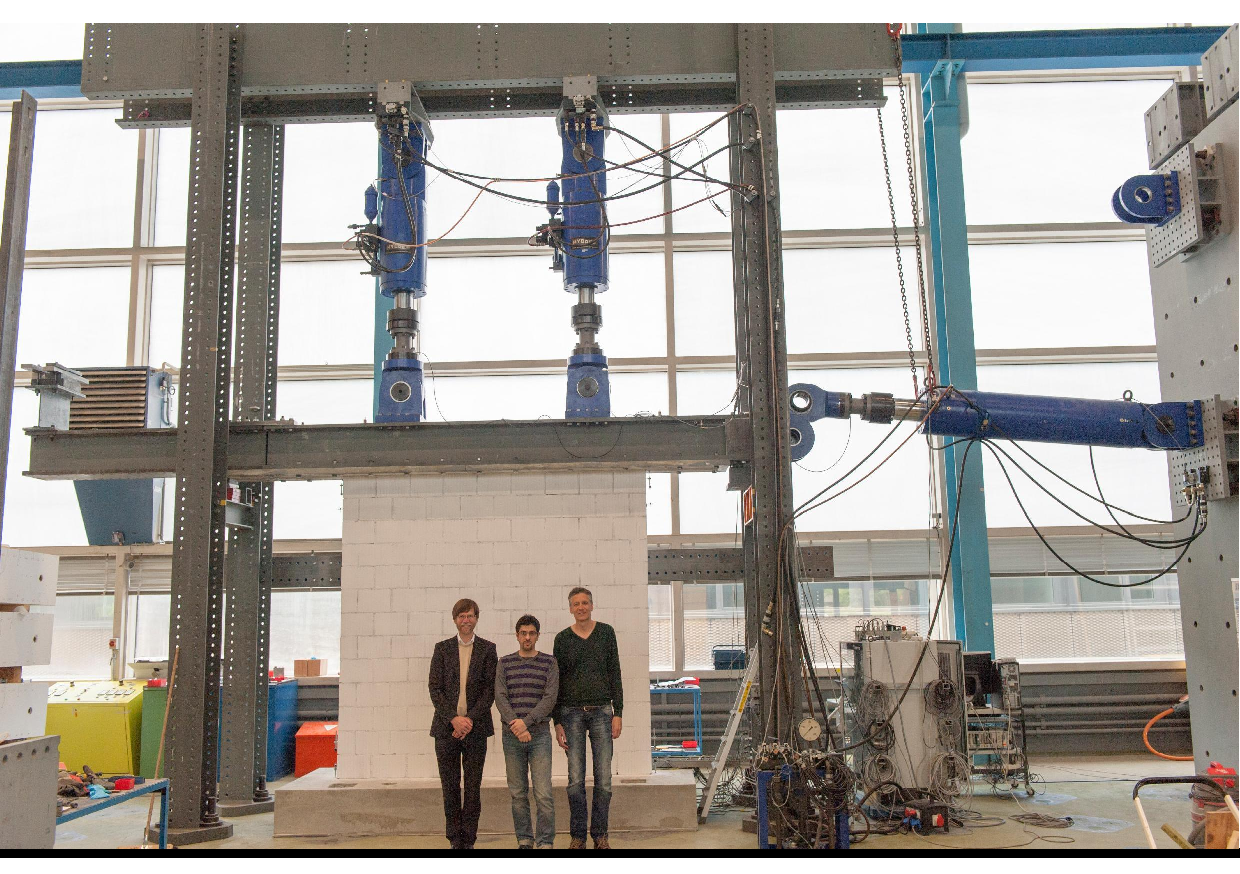
\includegraphics[width=\textwidth]{quasi_stati.pdf}
\caption{Falazat kvázi-statikus vizsgálata \cite{quasi}.}
\label{fig:quasi}
\end{figure}


A rázópad-vizsgálat a második legelterjedtebb formája a laborkísérleteknek. A valós földrengések alatti állapotokhoz hasonlót lehet szimulálni a vizsgálattal. A rázópad-kísérletek fontos adatokat szolgálnak a földrengésekre adott dinamikus válaszokról, figyelembe véve a vizsgált szerkezet inerciáit és energia-disszipációit, valamint a geometriai nemlinearitások, a korlátozott alakváltozások  és a szerkezeti elemek meghibásodásának következményeit. A módszer hátránya, hogy a teljes szerkezeti rendszert gondosan fel kell építeni. Másrészt viszont a  valós idejű dinamikus elem vizsgálat számos lehetőséget tartogat, azonban irányítása komoly kihívást jelent, mert a rázópad mozgatását ekkor aktuátorok végzik.  A rázópadok korlátozott méretei és kapacitása miatt a próbatestek mérete, súlya és teherbírása is jelentősen korlátozott, ennek eredményeként gyakran csökkentett méretű vagy nagyon leegyszerűsített próbadarabok válnak szükségessé, és ezért sokszor megkérdőjelezhetővé válnak a vizsgálati eredmények.
Az \ref{fig:shaking} ábrán egy hatszabadságfokú rázópad látható. A szerkezet a George Washington Egyetem (GWU) laboratóriumában található.

\begin{figure}[h!bt]
\centering
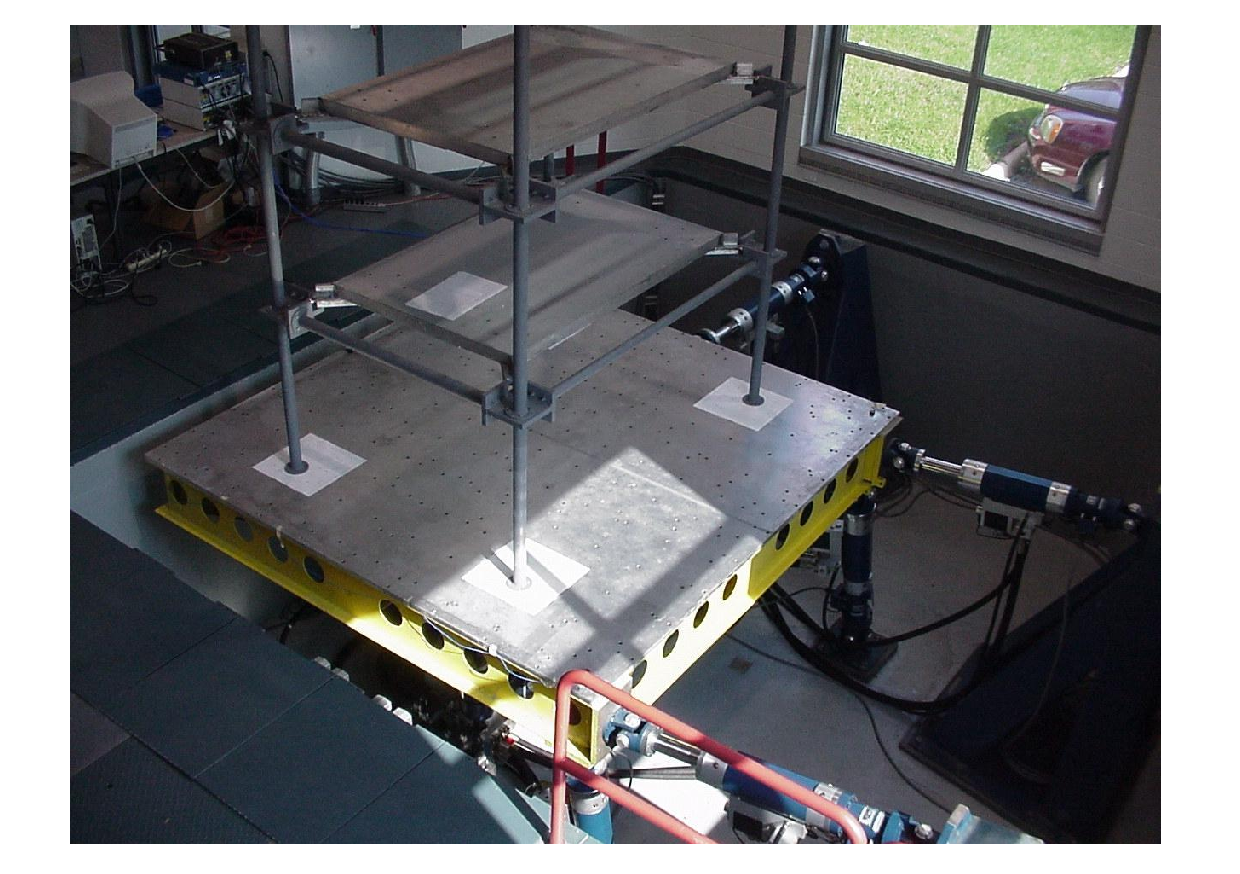
\includegraphics[width=\textwidth]{Shake_Table.pdf}
\caption{Hatszabadságfokú rázópad \cite{shaking}.}
\label{fig:shaking}
\end{figure}

A harmadik módszer a hibrid szimuláció, más néven pszeudo-dinamikus vagy csatolt számítógép-irányított vizsgálati módszer. Ebben a  kísérleti eljárásban a szimuláció egy olyan modellen van végrehajtva, ami figyelembe veszi a szerkezet numerikus és fizikai komponenseit is, és az erre felírt mozgásegyenletek  időlépéses numerikus megoldásán alapul. A hagyományos számítógépes modellezéssel és szimulációval ellentétben, ahol az egész szerkezet analitikusan van elemezve, a hibrid szimulációs módszerben  a szerkezeti rendszer erőjellegű mennyiségei dinamikus terhelés esetén (mint a merevség, energia-disszipáció vagy tömeg tulajdonságok)  a teljes szerkezetnek vagy egyes részeinek laboratóriumi vizsgálatával válnak ismertté. Ha a hibrid szimuláció egy szokványos kvázi-statikus elmozdulásalapú vizsgálatként van végrehajtva, a próbatest tömeg- és viszkózus csillapításjellemzői numerikusan modellezhetők, és a szerkezet meghatározott dinamikus gerjesztésének hatására keletkező elmozdulásnövekmények minden lépésnél a fizikai és numerikus modellek alapján számíthatók. A szimuláció során a teljes hibrid modell fizikai részei egy vagy több laboratóriumban vizsgálhatók számítógép-irányított aktuátor segítségével, és egyidejűleg a numerikus részek egy vagy több számítógépen analizálhatók. Mivel a szimuláció dinamikus aspektusai numerikusan vannak kezelve, az ilyen vizsgálatok kvázi-statikusan végezhetők hagyományos számítógép-irányított aktuátort használva. A hibrid szimulációt ezért úgy is lehet tekinteni, mint egy speciális aktuátor alapú vizsgálatot, ahol a terheléstörténet egy kísérlet során van meghatározva, melyben a szerkezet adott földmozgásnak van alávetve. Másrészről a hibrid szimuláció felfogható hagyományos végeselemes vizsgálatnak is, ahol a numerikus modellbe be van ágyazva a szerkezet egyes részeinek fizikai modellje. Az \ref{fig:hibridkep} képen egy hibrid szimulációs vizsgálat elrendezése látható két egymástól függetlenül mozgatható próbatest esetén, a \ref{fig:lehigh_szerk} képeken  pedig a Lehigh Egyetemen végzett kísérlet felállítása látható, ahol   magnetoreológiai csillapítók (MR dampers) beépítésének hatását vizsgálták acélvázas épületek viselkedésében.

\begin{figure}[h!bt]
\centering
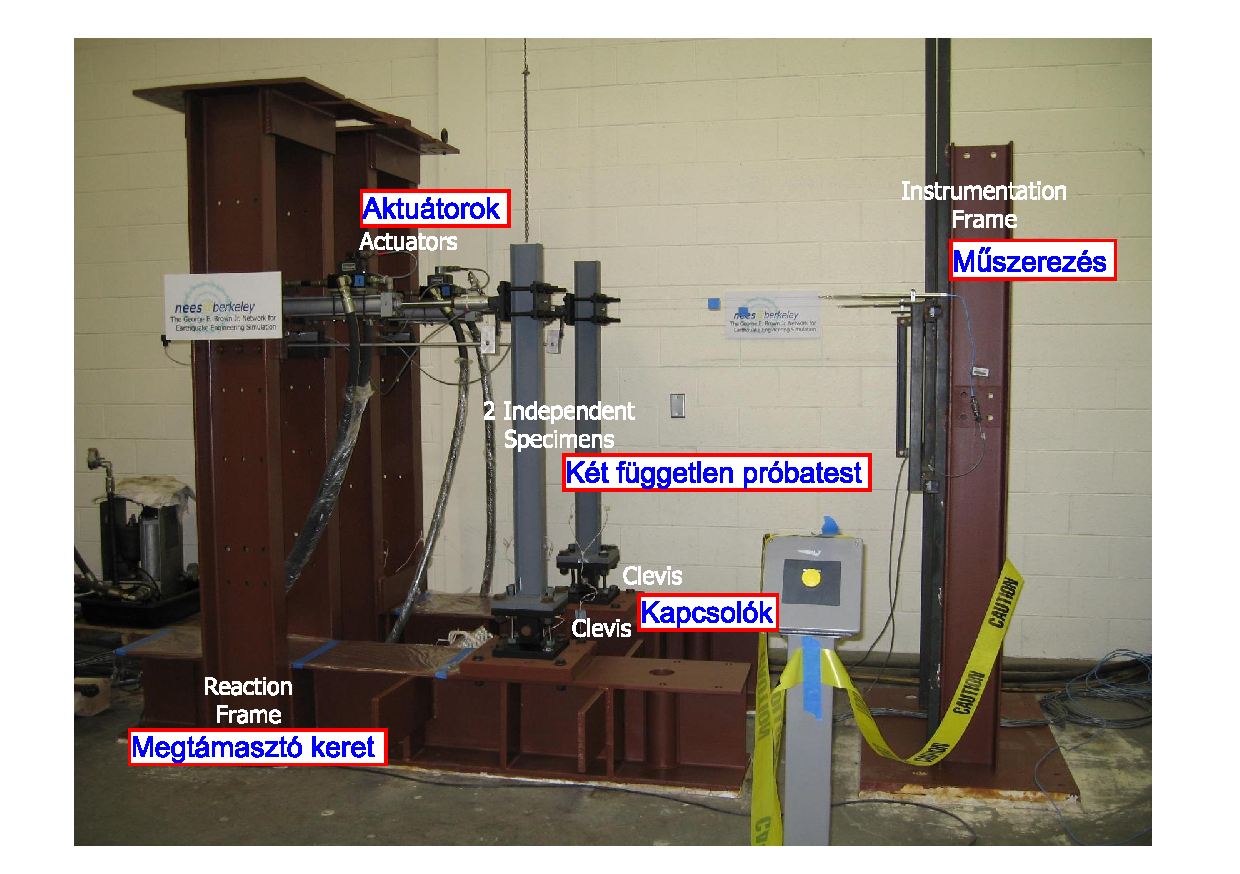
\includegraphics[width=\textwidth]{hibrid_alkalmazas.pdf}
\caption{Hibrid szimulációs kísérlet \cite{hibrid}.}
\label{fig:hibridkep}
\end{figure}


\begin{figure}[p]%
\centering
\subfigure{%
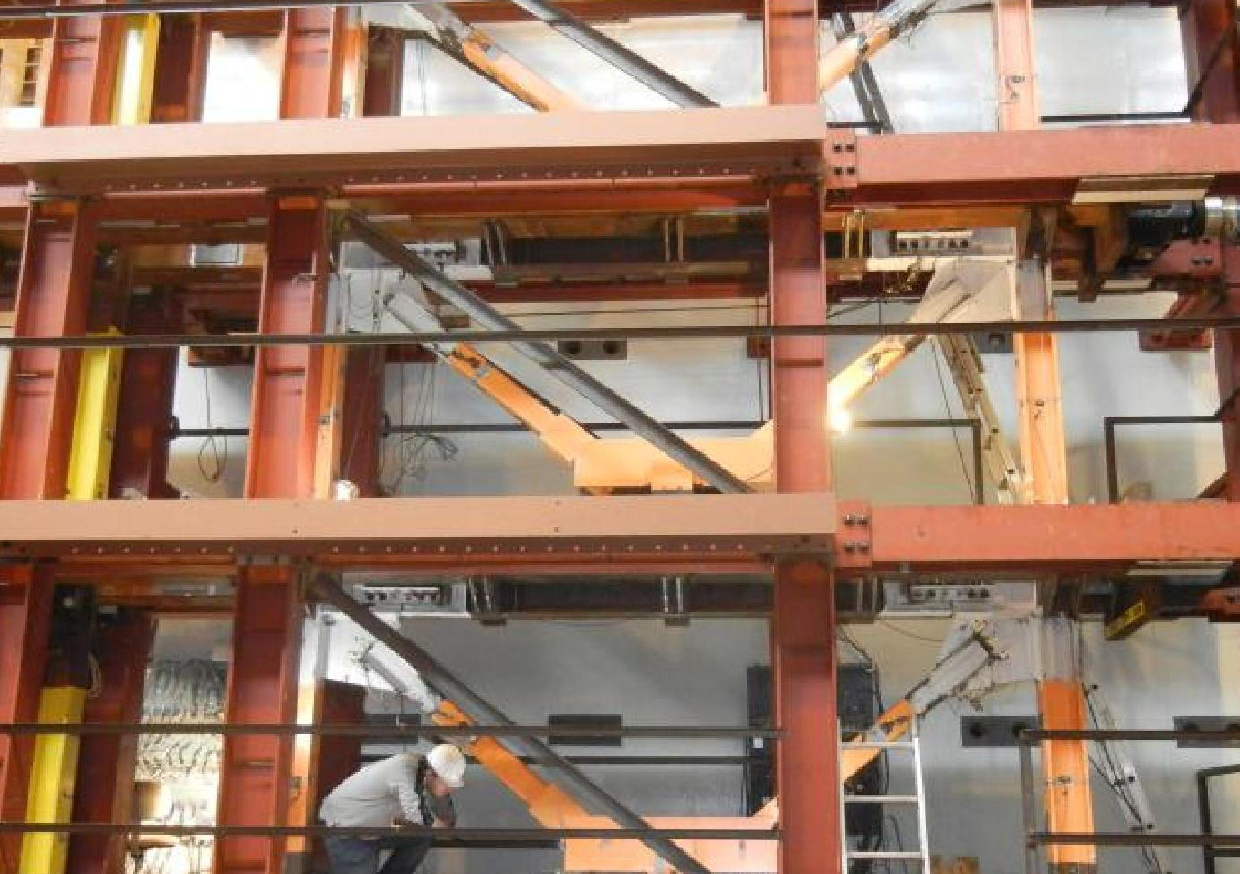
\includegraphics[width=\textwidth]{lehigh_2.pdf}}%
\\
\subfigure{%
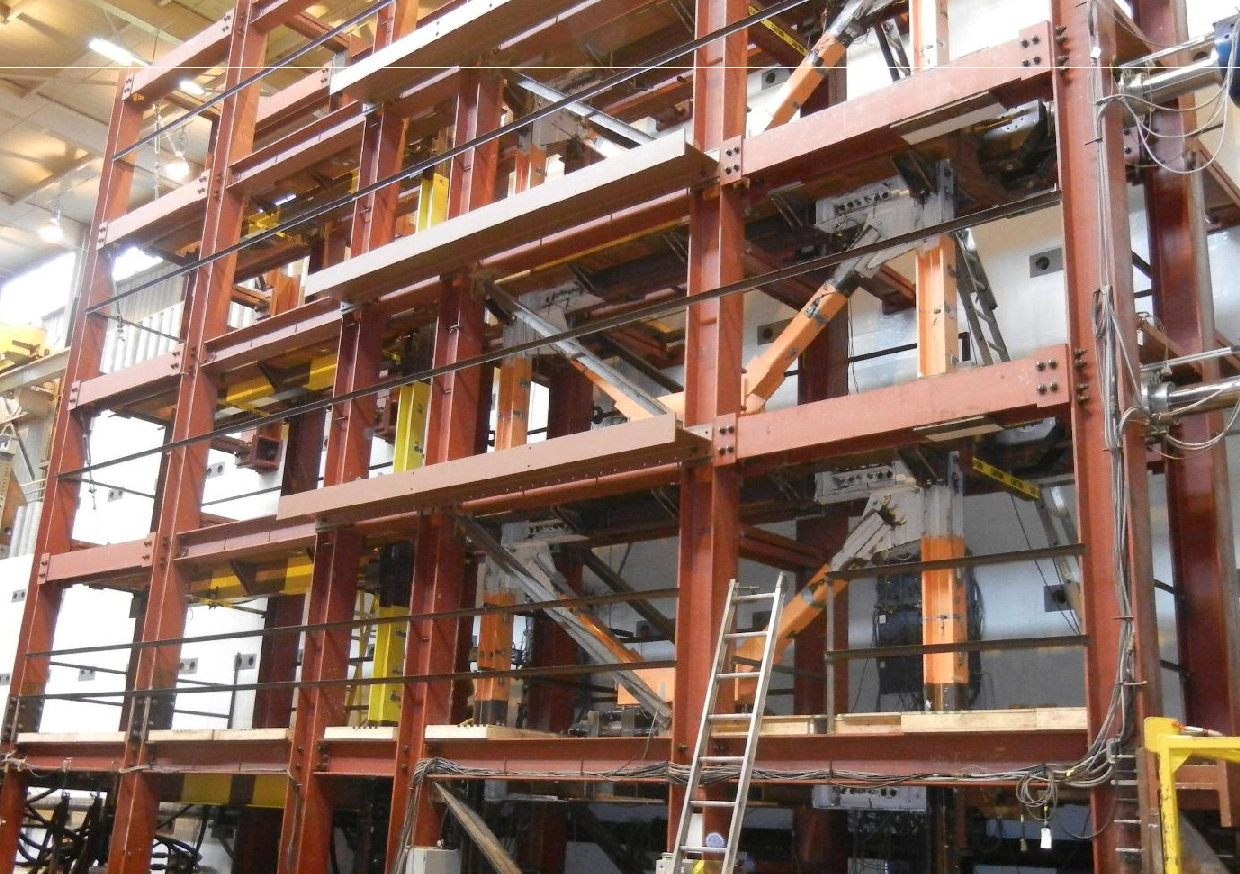
\includegraphics[width=\textwidth]{lehigh_1.pdf}}%
\caption[A Lehigh Egyetemenen végzett hibrid szimulációs kísérlet.]{A Lehigh Egyetemenen végzett hibrid szimulációs kísérlet elrendezése \cite{lehigh}.}
\label{fig:lehigh_szerk}%
\end{figure}


\newpage
\section{Előnyök és kihívások}
{\ }

A következőkben  a hibrid szimuláció főbb előnyeit mutatom be a kvázi-statikus és a rázópados vizsgálattal szemben. Emellett összefoglalom  azt a számos kihívást is, amellyel a jövőben foglalkozni kell a hibrid szimuláció kapcsán.


\subsection{Előnyök}

{\ }

A hibrid szimulációs eljárás számos előnnyel rendelkezik, mivel  a szerkezeti rendszer vizsgálatának ötvözi az analitikus és  kísérleti megközelítését, és a végrehajtható időlépték  maximum két nagyságrenddel lassabb a tényleges időléptéknél. A következő lista összefoglalja a legfontosabb előnyöket:
\begin{itemize} 
\item Egy hibrid szimulációban a teher (vagyis a mozgásegyenlet jobb oldala) analitikusan van definiálva, ami a legkülönbözőbb terhelési feltételek mellett gerjesztett szerkezetek viselkedésének vizsgálatát teszi lehetővé. A szeizmikus események, a hullámok okozta hidrodinamikus terhek, mozgó járművek miatti közlekedési terhek, szél általi aerodinamikai és a robbanásterhek mind szimulálhatók az analitikus részbe való beépítéssel, a kísérlet fizikai részeinek megváltoztatása nélkül.
\item Hibrid szimulációban lehetőség van arra, hogy egy nagyobb szerkezet részegységekre, vagyis alszerkezetekre legyen bontva: (1) a numerikus alszerkezethez a jól megértett viselkedésű szerkezeti elemek tartoznak, amelyekre biztonságosan felállítható a végeselemes modell , (2) a fizikai alszerkezethez pedig az erősen nemlineáris viselkedésű vagy numerikusan nehezen szimulálható szerkezeti elemek tartoznak, ezért ezek laboratóriumban vannak vizsgálva. A numerikus modell valós fizikai komponenssel való helyettesítése csökkenti a modellezés bizonytalanságait. A hibrid szimuláció ezért tekinthető a szerkezeti összetevők vizsgálatának egy speciális formájának is, amelynél nem kell kielégíteni olyan szigorú peremfeltételeket, mint a rázópados vizsgálatnál.
\item A teljes méretű próbatestek dinamikus vizsgálatára is lehetőség nyílik, amennyiben a hibrid szimuláció átlagos kvázi-statikus elmozdulásalapú vizsgálatként valósul meg, kiterjesztett időléptékkel végrehajtva. Továbbá a nagyméretű vizsgálatoknál megszűnnek a méretezés során felmerült nehézségek, amik a rázópadvizsgálatnál fennálltak.
\item A fizikai részegységek mérete és súlya csak a rendelkezésre álló laboratóriumi terület a padló és a megtámasztás  teherbírásától függ. Továbbá a próbatest teherbírását csak az átviteli rendszer (aktuátor) kapacitása korlátozza.
\item Mivel a hibrid szimuláció nagyobb időléptéken is végrehajtható, a kvázi-statikus vizsgáló berendezések, mint az aktuátorok, a szervoszelepek, és a hidraulikus tápegység, általában elegendőek a vizsgálathoz. Gyakran az ilyen berendezések rendelkezésre is állnak a vizsgálati létesítményekben. Ezért és amiatt, hogy fizikailag  csak a szerkezeti rendszer kritikus elemei vannak vizsgálva, a hibrid szimuláció nagyon gazdaságos laboratóriumi vizsgálati eljárás.  
\item A lassú tesztek lehetővé teszik a próbatestek pontos vizsgálatát a szimuláció közben. Lehetővé teszi a próbatest viselkedésének gondosabb megfigyelését, a károsodások megindulásának észlelését és a folyamat nyomon követését a szimuláció alatt.
\item Hibrid szimulációt a valós időléptéknél kétszer lassabb, és sokszor gyorsabb intervallum között bárhol végezhetünk a hasonlósági követelményeknek megfelelően.
\item A numerikus és a kísérleti alszerkezetek földrajzilag eloszthatók, így a szimuláció akár több különböző laborban is futhat, kihasználva a helyszínek adottságait. 
\item Az olyan hatásokat, mint a geometriai nemlinearitások, a háromdimenziós hatások, a talaj-szerkezet kölcsönhatások valamint a talajmegtámasztás hatása, mind a modell analitikus részébe kell foglalni.
\item Hibrid szimuláció alkalmazható intelligens rázópad vizsgálathoz, amelyben a szimulátor padozat valós időben irányított, olyan problémák vizsgálatára, mint a hangolt csillapító tömeg vagy a talaj-szerkezet kölcsönhatás.
\end{itemize} 

\subsection{Kihívások}

{\ }

Számos előnye és lehetősége mellett a hibrid szimulációnak szembesülnie kell számos kihívással is, ezért további kutatásokat kell folytatni a vizsgálattal kapcsolatban, és  speciális szimulációkat kell elvégezni az eredmények értékelésére és verifikálására. Néhány ilyen kihívást foglal össze a következő lista:
\begin{itemize}
\item A hibrid szimuláció fejlesztését és telepítését akadályozza a közös keretrendszer hiánya a  különböző laboratóriumokban és számítástechnikai környezetben végrehajtott vizsgálatokhoz. A vizsgálatok problémaspecifikusak, és erősen függnek a vizsgálat helyszínétől és a használt irányító- és adatgyűjtő rendszertől. Az ilyen rendkívül egyedi szoftver megvalósításokat nehéz különböző szerkezeti problémákra alkalmazni, és még nehezebb különböző laboratóriumokba átvinni. Ezért nagy szükség van egy olyan környezetfüggetlen szoftver-keretrendszerre, amely nagy teljesítményű, átlátható és könnyen bővíthető.
\item Annak biztosítására, hogy a kapott eredmények érvényesek, megbízhatóak és pontosak legyenek, rendkívül fontos, hogy a megoldás hibák miatti pontatlanságai minimalizálva, illetve javítva legyenek. A következő hibák fordulhatnak elő különböző szinteken a szimuláció során, melyek befolyásolhatják a megoldási folyamatot: (1) a diszkretizálás folyamata és az energia-disszipációról való feltételezések  miatti modellezési hibák; (2) az integráló és egyensúlyi megoldó algoritmusok okozta numerikus hibák; (3) a irányító- és átviteli rendszerek által generált kísérleti hibák; végül (4) a műszerezés és az adatgyűjtő rendszer által okozott kísérleti hibák. A kísérleti hibák energiatöbbletet vezethetnek a hibrid rendszerbe, ezáltal instabillá teszik azt,  ezért nagyon fontos minimalizálni vagy kompenzálni ezeket.
\item Az olyan hibrid szimulációk végrehajtása, ahol komplex analitikai alkotóelemek, mint az anyagi és geometriai nemlinearitások,  komplex,  rugalmatlan kísérleti alkotóelemekkel vannak kombinálva, meglehetősen bonyolult feladat. Ennek oka, hogy ezek a modellek általában implicit, iteratív integráló formulák használatát követelik, amikben a megoldási folyamat során folyamatosan ellenőrizni  kell, hogy a megoldás konvergál-e. Ráadásul a számítógépes terhelések a nemlinearitások miatt jelentősen eltérhetnek két időlépés között, megnehezítve, vagy lehetetlenné téve  a  gyors és valós idejű szimulációk végrehajtását.
\item A nagyon merev vagy felkeményedő fizikai alépítményt tartalmazó hibrid szimulációkat nehéz teljesíteni elmozdulásirányítás alatt. Ezért szükséges kihasználni az erőirányítást, a kevert erő- és elmozdulásirányítást vagy a szimuláció alatti kapcsolást az erő- és elmozdulásirányítás között. Eddig nagyon kevés kutatást végeztek ezen a területen.
\item Szükség van olyan  megközelítések kidolgozására, amik következetesen alkalmazzák a hasonlósági törvényeket akkor is, ha a szerkezeti rendszer  analitikus és kísérleti része különböző léptékű.
\item Földrajzilag elosztott hibrid szimulációk megkívánják a hálózati késésekkel és meghibásodásokkal foglalkozó, valamint a kommunikáció sebességét javító eszközöket. Ezek a funkciók elengedhetetlenek a gyenge valós idejű, földrajzilag elosztott hibrid szimulációk elvégzéséhez, ahol a valós idejű követelményeket átlagos értelemben kell kielégíteni, de nem szükséges minden egyes időlépésben. 
\item Egy másik kihívás olyan módszerek fejlesztése, amik a hibrid szimuláció pontosságát  és hatékonyságát értékelik. Ezen módszereknek lehetővé kell tenniük, hogy a hibrid szimuláció ne csak a befejezése után, hanem már a szimuláció közben is értékelhető legyen. 
\item Ahogy a hibrid modellek egyre nagyobbá válnak (egyre nő a csomópontok, elemek és szabadsági fokok száma), egyre bonyolultabbak lesznek (egyre több az anyagi és geometriai nemlinearitás), és a közel vagy ténylegesen valós idejű  vizsgálatok elterjednek, a nagy teljesítményű számítástechnikai  (High-Performance Computing - HPC)  környezet egyre nélkülözhetetlenebbé válik a hibrid szimulációk végrehajtásához. Nagy teljesítményű számítástechnikai környezetben hasznosítani lehet a többprocesszoros és/vagy többmagos párhuzamos számítástechnikai képességeket a munkaterhelés elosztására és ezáltal a teljesítmény javítására. 
\item A gyors és valós idejű hibrid szimulációkban a tehetetlenségi erőket, amik a kísérleti alkotóelemek  fizikai tömegeiből származnak, nem szabad elhanyagolni. Tehát fontos az olyan módszerek fejlesztése, amik megfelelően veszik figyelembe  ezeknek az erőknek a hozzájárulását.
\item Azért, hogy a hibrid szimuláció elérhetősége a kutatói közösség számára javuljon, hathatós, de mégis közérthető felhasználói felületet kell kidolgozni.
\end{itemize}

\section{Az eljárás  összetevői}

{\ }

A hibrid szimuláció végrehajtásához számos kulcsfontosságú összetevőre van szükség, beleértve a szoftver és hardver komponenseket is. Ezek a szimuláció során mind interakcióba lépnek. A hibrid szimuláció kulcselemeit ábrázolja a \ref{fig:hibridszim}-es ábra, és a következőkben rövid bemutatásuk olvasható.

\begin{figure}[h!]
\centering
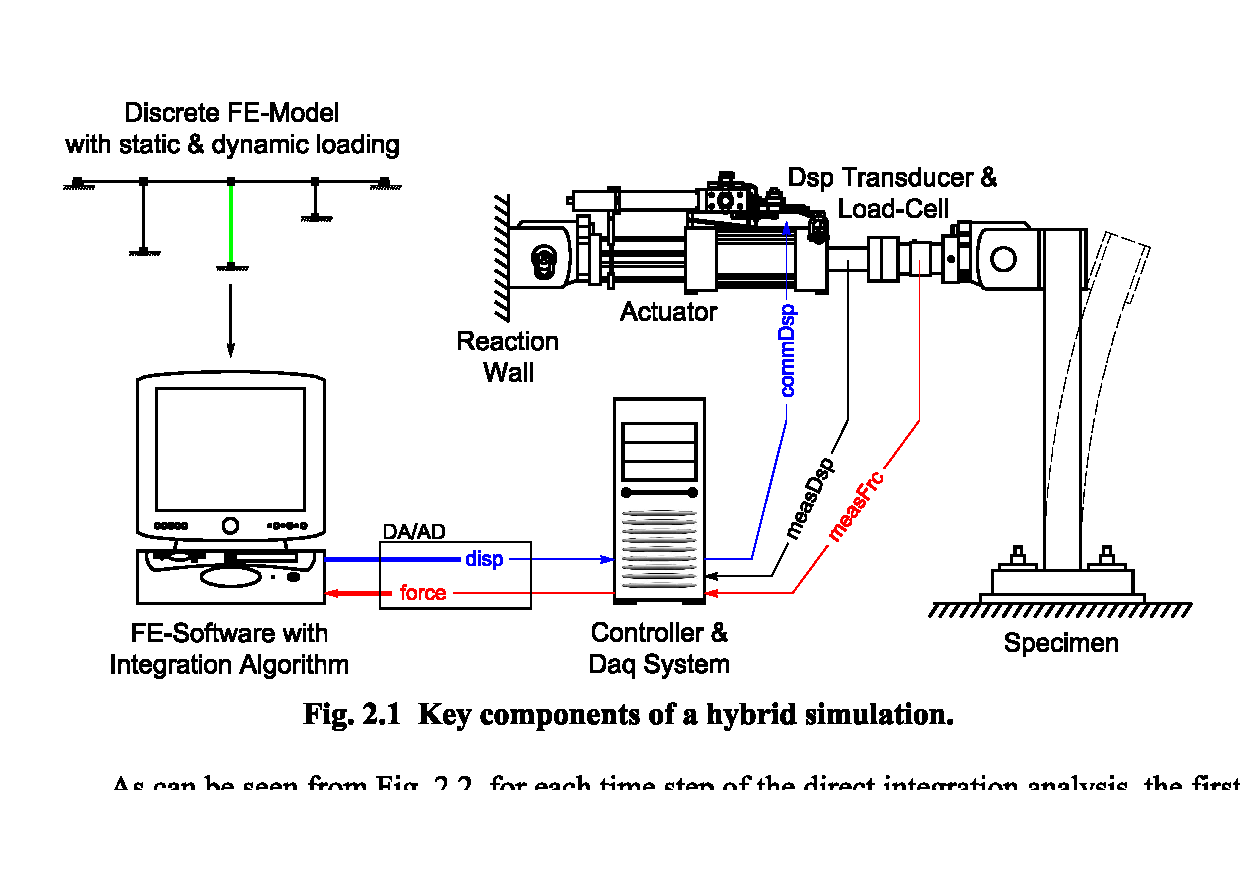
\includegraphics[trim = 0mm 30mm 0mm 0mm, clip, width=\textwidth]{hibridszim.pdf}
\caption[A hibrid szimuláció kulcselemei \cite{hibrid}]{A hibrid szimuláció kulcselemei \cite{hibrid}.(Az egyes elemek jelentésének fordítását és magyarázatát a főszöveg tartalmazza.)}
\label{fig:hibridszim}
\end{figure}

\begin{enumerate}
\item Az első komponens  a szerkezet számítógépen analizálandó diszkrét végeselemes modellje, ami tartalmazza a statikus és dinamikus terhelést is (az \ref{fig:hibridszim} ábrán: Discrete FE-Model with static and dynamic loading).  A szerkezeti analízis itt bemutatott megközelítése szerint végeselemes módszer használatos a térbeli, és  időlépéses módszer az időbeni diszkretizálásra (az \ref{fig:hibridszim} ábrán: FE-Software with Integration Algorithm). Az alternatív irányított rendszerrel való megközelítéssel összehasonlítva a végeselemes megközelítés a szerkezetépítő mérnök számára sokkal intuitívabb és könnyen kiterjeszthető megosztott hibrid szimulációk elvégzésére. A dinamikus mozgásegyenletek véges számú diszkrét szabadságfokra felírása  egy másodrendű közönséges differenciálegyenlet-rendszert eredményez, melynek szabad változója az idő.
\begin{equation}
\mathbf{M}\mathbf{\ddot{U}}_{i+1}+\mathbf{C}\mathbf{\dot{U}}_{i+1}+\mathbf{f}_s(\mathbf{U}_{i+1}) = \mathbf{P}_{i+1}-\mathbf{P}_{0,i+1}
\label{hibrid alapegyenlet}
\end{equation}
Az \eqref{hibrid alapegyenlet} egyenlet az időben diszkretizált differenciálegyenlet-rendszer a $t = t_{i+1}$ időpontra felírva, ahol az $\mathbf{M}$ a csomóponti és elemi tömegmátrixokból összeállított tömegmátrix, $\mathbf{\ddot{U}}_{i+1}$ a gyorsulásvektor a $t_{i+1}$ időpontban, $\mathbf{C}$ a képlékeny csillapítási mátrix, $\mathbf{\dot{U}}_{i+1}$ a sebességvektor a $t_{i+1}$ időpontban, $\mathbf{f}_s$ a rugalmas visszatérítő erő  az $\mathbf{U}_{i+1}$ a $t_{i+1}$ időpontban vett elmozdulásvektor függvényében, $\mathbf{P}_{i+1}$ a külső csomóponti terhek  és $\mathbf{P}_{0,i+1}$ az elemek terhei a $t_{i+1}$ időpontban.

A \ref{sec:idolepmsz} pontban bemutatott lineáris időlépéses integráló módszerek közül a \eqref{hibrid alapegyenlet} mozgásegyenlet megoldására a CR algoritmus a legalkalmasabb. A explicit, feltétel nélkül stabil eljárást a valós idejű hibrid szimulációkhoz fejlesztették, irányításelméleti módszerek alkalmazásával. 

\item A második szükséges komponens egy átviteli rendszer (Transfer System), amely egy irányítóból  és statikus vagy dinamikus aktuátorokból áll (az \ref{fig:hibridszim} ábrán: Controller, Actuator), így az időlépéses integráló formulákkal meghatározott (általában elmozdulás) növekményválaszokat alkalmazni lehet  a fizikai alépítményen. Lassú vizsgálatoknál felhasználhatók a kvázi-statikus vizsgálatokhoz is alkalmazott, relatíve olcsó eszközök. Ezek gyakran rendelkezésre állnak a szerkezetvizsgáló laboratóriumokban.

\item A harmadik fő komponens a laborban tesztelt  kísérleti próbatest, beleértve a támaszokat is (az \ref{fig:hibridszim} ábrán: Specimen, Reaction Wall), amivel az átviteli rendszer aktuátorai kapcsolódnak.

\item A negyedik és egyben utolsó komponens egy adatgyűjtő rendszer (az \ref{fig:hibridszim} ábrán: Daq System), amely olyan elemeket tartalmaz, mint az elmozdulás jeladók, az erőmérő cellák (az \ref{fig:hibridszim} ábrán: Dsp Transducer \& Load-Cell) és a gyorsulásmérők (Accelerometers). Az adatgyűjtő rendszer felelős a próbadarab válaszának méréséért és kísérleti adatként való továbbításáért a numerikus alépítmény felé, hogy a következő időlépéshez tartozó megoldás számítható legyen.
\end{enumerate}

 A hibrid szimulációs eljárásokra fejlesztették az OpenFresco (Open-source Framework for Experimental Setup and Control) környezetfüggetlen szoftver keretrendszert. Az OpenFresco  a hibrid szimulációs eljárásokban a végeselemes modellt köti össze az irányító és adatgyűjtő rendszerrel, így megkönnyíti a laboratóriumi kísérletek  elvégzését. A végeselemes modell készítésére ebben a környezetben a legelterjedtebb az OpenSEES szoftver. A programot kifejezetten szerkezetek viselkedésének vizsgálatára fejlesztették földrengés hatására  alatt.

%Mivel a szimuláció kulcselemei végeselemes megközelítés alkalmazásával lettek bemutatva,  adott a direkt integrálás végrehajtásának szempontjából  szükséges  vizsgálati eljárás. Az eljárás részleteinek egyszerűsítése végett a nemlineáris helyett lineáris egyensúlyi megoldó algoritmus kerül alkalmazásra. A vizsgálati eljárás folyamatábráját mutatja a \ref{hibrid folyamat}-es ábra. 

%Amint a \ref{hibrid folyamat}-es ábrából látható, a direkt integrálás minden egyes időlépésében az első művelet az új próba válaszmennyiségek (elmozdulások, sebességek és gyorsulások) meghatározása. Ezután a terhelés és a vizsgálati idő növekszik, és az új próba válaszmennyiségek lesznek elküldve  az analitikus és a kísérleti alszerkezetnek. Az analitikus alszerkezet tárolja az új válaszmennyiségeket, így ezek később meghatározhatják a kiegyensúlyozatlan terheket. Másrészt  a kísérleti alszerkezet kommunikál az átviteli rendszerrel a laborban, ami elkezdi az új elmozdulásokat végrehajtani.

\section{A helyi és a földrajzilag megosztott eljárás összehasonlítása}

{\ }

Ha a hibrid szimuláció előnyeit felsorakoztatjuk, láthatjuk, hogy  egy nagyon sokoldalú vizsgálati módszer, és ez sok különböző alkalmazási módot tesz lehetővé. Ezért érdemes kategorizálni a fő alkalmazási módokat és meghatározni a hozzájuk  kapcsolódó fogalmakat.

A kategorizálás első módja a szerkezeti alegységek és a különböző elemek  csoportosítása földrajzi megosztottságuk szerint. A helyi vagy lokális hibrid szimulációban a numerikus analízis és a kísérleti vizsgálat elvégzése ugyanazon a helyen, vagyis ugyanabban a laboratóriumban történik.  Mivel a végeselemes analízis  hardvere, az irányító rendszer, az adatgyűjtő rendszer mind ugyanott helyezkedik el, a csatlakozásuk megoldható helyi nagysebességű hálózati körön keresztül. Ezek drasztikusan csökkentik a késedelmeket, és lehetővé teszik a folyamatos vagy akár a valós idejű hibrid szimulációk végrehajtását. Így a helyi hibrid szimulációnak többnyire nem akadálya a szerkezeti egységek közötti kapcsolat hiánya, viszont az összes szükséges alkatrész egy laboratóriumban való elhelyezése komoly nehézségekbe ütközhet.

Ezzel szemben a földrajzilag megosztott hibrid szimulációban a szerkezet különböző részei különböző helyszíneken vannak vizsgálva és  elemezve. Ez azt jelenti, hogy a modell analitikus részei egyszerre több számítógépen is elemezhetők, és  a hibrid modell fizikai részei egyszerre több laboratóriumban is vizsgálhatók. Mivel néhány vagy az összes alegység szétszórtan helyezkedik el,  összekapcsolásukra csak nagy kiterjedésű hálózatok használhatók. Ezek általában nagyobb késéseket okoznak, mint a helyi nagysebességű hálózatok, így a gyors hibrid szimulációk végrehajtása  nagy kihívást jelent. Ráadásul szükség van egy eszközre, ami a túlzottan nagy hálózati késésekkel és a meghibásodásokkal foglalkozik. Azonban a modell  kijelölt alegységekre bontásával valamint laboratóriumok és számítási helyek hálózatán belüli eloszlásával  lehetőség nyílik a különböző adottságú helyszínek optimális kihasználására. 

\section{A lassú, a gyors és a valós idejű vizsgálatok összehasonlítása}

{\ }

A hibrid szimuláció másik fontos jellemzője  a vizsgálat végrehajtásának sebessége. A lassú vizsgálatokat a valós időléptéknél  akár két nagyságrenddel nagyobb időléptékkel hajtják vére,  míg a valós idejű vizsgálatokat a tényleges időléptékkel azonos vagy annál kisebb időléptékkel kell elvégezni a hasonlósági követelményektől függően. Így a hibrid szimuláció különböző aspektusait a végrehajtás sebességének függvényében alaposabban kell figyelembe venni és kezelni. A lassú vizsgálatnál nagyon fontos, hogy a fizikailag vizsgált szerkezeti részek nem mutathatnak sebességfüggő viselkedést kivéve, ha ezt az analitikus részben kompenzálják. Ezenkívül fontos az  aktuátor folytonos mozgásával járó megszakítás nélküli végrehajtás, a relaxációs erő és a rúd szétcsúszásának elkerülése érdekében. Másrészt a gyors hibrid szimulációhoz elengedhetetlen a fizikai részek által generált  tehetetlenségi és  csillapító erők megfelelő számítása vagy kompenzálása. Emellett fontos annak felismerése, hogy az ilyen vizsgálatokhoz nagy erejű dinamikus aktuátorok nagy akkumulátorral és hidraulikus szivattyú rendszer szükségesek, ezáltal az aktuátorok pontos irányítása sokkal nehezebbé válik a tehetetlenségi erő visszacsatolások miatt.

A hibrid szimuláció során megoldandó mozgásegyenletek némileg eltérő formákat vesznek fel a végrehajtás sebességétől függően. A lassú teszteknél nem keletkeznek tehetetlenségi erők a fizikai alegységekben, ezért az egész szerkezet tömeg és viszkózus csillapítási mátrixa numerikusan kezelhető, ugyanis a kísérleti visszatérítő erő  nem tartalmaz semmilyen inerciális vagy viszkózus csillapító erő hozzájárulást.  Így a tömeg és a csillapítási mátrix közvetlenül előállítható  az analitikus és kísérleti alszerkezet  csomópontjainak és szerkezeti elemeinek együttes figyelembevételével. 
 
Ezzel ellentétben, ha a hibrid szimulációt gyorsabban hajtják végre,  tehetetlenségi és viszkózus csillapító erők keletkeznek a szerkezet fizikailag vizsgált részeiben, ezeket figyelembe kell venni a kísérleti visszatérítő erő vektorában. A visszatérítő erő számításához szükséges tömeg és csillapítási mátrixokat a kísérleti alszerkezet alapján állítjuk össze, a gyorsulások és sebességek vektorait pedig a kísérleti részeken mérjük.

Ha elérjük a valós idejű sebességet, a kísérleti alszerkezetre a  számított gyorsulások és sebességek hatnak (a hasonlósági követelmények figyelembevételével). Így a mozgásegyenletben a tömeg és csillapítási mátrixokat elég csak a numerikus alszerkezetből számolni, a visszatérítő erőt pedig elég a kísérleti alszerkezet alapján előállítani, ami tartalmazza a szerkezet fizikai részeinek tehetetlenségi és csillapítási erőit. A kísérleti visszatérítő erő vektor teljes egészében előállítható a mért erők értékeiből. Viszont ha a valós idejű szimulációt intelligens rázópadkísérlethez alkalmazzák, ahol  nagyobb alegységeket vizsgálnak a kísérleti platón, a kísérleti visszatérítő erő nem a relatív válaszmennyiség függvénye, ehelyett az abszolút válaszmennyiséget kell a rázópad irányító rendszerének küldeni.  



\section{A hibrid szimuláció értékelése}

{\ }

Tanulmányomban bemutattam a hibrid szimulációs eljárást, és ismertettem előtérbe kerülésének okait. Összefoglaltam az előnyeit más kísérleti eljárásokkal szemben, valamint a szimuláció megvalósításához kapcsolódó kihívásokat. Bemutattam az eljárás kulcselemeit, és azt, hogy milyen műszerekkel valósítható meg. Jellemeztem az eljárást földrajzi megosztottság  és a szimuláció sebessége szerint. Ezek  alapján a hibrid szimulációs eljárás pontos, viszonylag könnyen megvalósítható, könnyen variálható  és költséghatékony kísérleti módszer, ami alkalmas a nagyobb építőmérnöki szerkezetek dinamikus teljesítményének vizsgálatára. 

 A következő fejezetben bemutatom a hibrid szimulációs eljárásra fejlesztett programomat. A valós idejű  szimulációk végrehajtására a CR algoritmus a legalkalmasabb, így  a programban én is ezt  alkalmaztam a numerikus számítások végrehajtására.













\chapter[Hibrid szimulációs program]{Hibrid szimulációs program fejlesztése és verifikálása}\label{chap: hibrid progi}

{\ }

Ebben a fejezetben az általam fejlesztett hibrid szimulációs program működését és használatát mutatom be, majd elvégzem a program verifikálását. A programot a \ref{chap: lin+nemlin progi}. fejezetben ismertetett lineáris és a nemlineáris megoldókhoz hasonlóan  MATLAB programnyelven írtam. Választásomat továbbra is azzal indokolom, hogy a MATLAB szoftver a legalkalmasabb a mátrixműveletek gyors és pontos elvégzésére, és ez a  nagy méretű mátrixokkal való számításokra is igaz. 

A programom egy szimulált hibrid szimulációs program, ami átalakítható valós hibrid szimulációs programmá. Ennek oka, hogy hibrid szimulációs kísérletek jobb megértése érdekében a  laborban történő alkalmazása előtt érdemes a kísérleti vizsgálatokat szimulálni. A program szerkezete így könnyebben átalakítható és továbbfejlesztető. 

A program feladata, hogy a hibrid szimuláció módszerét szemléltesse, és hogy a hibrid szimulációs kísérlettel végzett számítások pontosságát igazolja. A programhoz felhasználtam a lineáris és nemlineáris megoldóknál bemutatott műveleti blokkokat is. A numerikus számításokhoz a \ref{sec:idolepmsz} pontban bemutatott integráló algoritmusok közül a \ref{subsec:cr} alatt ismertetett Chen-Ricles (CR) algoritmust használja. A \ref{chap: hibrid alk}. fejezetben  alkalmazom a programot egy szeizmikus szigeteléssel ellátott épület viselkedésének vizsgálatára. A program kódját a Függelék \ref{chap: függ hibrid prog}. fejezet tartalmazza.


\section{Program szerkezete}\label{hibrid prog szerk}

{\ }

A program folyamatábrája a \ref{fig:hibridprog_folyamatabra} ábrán látható. Az indítás előtt  kézzel meg kell adni  a rendszert leíró bemeneti adatokat. Az indítást követően az első lépés   a szerkezeti rendszert és a feladatot leíró mátrixok inicializálása,  amit  a számításhoz szükséges, a vizsgálat közben állandó segédmátrixok előállítása, valamint az időlépésenként  számítandó mátrixok helyfoglalása  követ. Ezután egy for ciklus következik amiben a vizsgálat előre megadott időintervalluma alatt a laboratóriumi kísérletek és a numerikus számítások folyamata zajlik. A program minden időlépésben konvertálja a laborba a kísérleti próbatestre alkalmazandó elmozdulásokat,  és beolvassa  a próbatest nemlineáris  válaszát. Ezt követően a laboreredményeket felhasználva először számítja az aktuális gyorsulást  a mozgásegyenletből, majd a  következő időlépésben alkalmazandó elmozdulást számolja a CR algoritmussal,  és tárolja azt. Végül vizsgálatot követően a program kirajzolja az eredményül kapott diszkrét elmozdulásvektorokat a vizsgálat teljes időintervallumára.

 Hibrid szimuláció esetében a laborban a próbatestet egy időlépés alatt több lépcsőben terhelik. Erre azért van szükség, hogy a szerkezet terhelésében ne legyen szünet. Minden időlépésben az utolsó előtti teherlépcsőnél kapott adatokat extrapoláljuk, és a terhelés utolsó szakasza közben a program elvégzi a következő időlépésben történő terheléshez  szükséges számításokat, és az eredmények konvertálását, így nem kell megakasztani a kísérletet a számítások miatt.
 
  

\begin{figure}[h!]
\centering
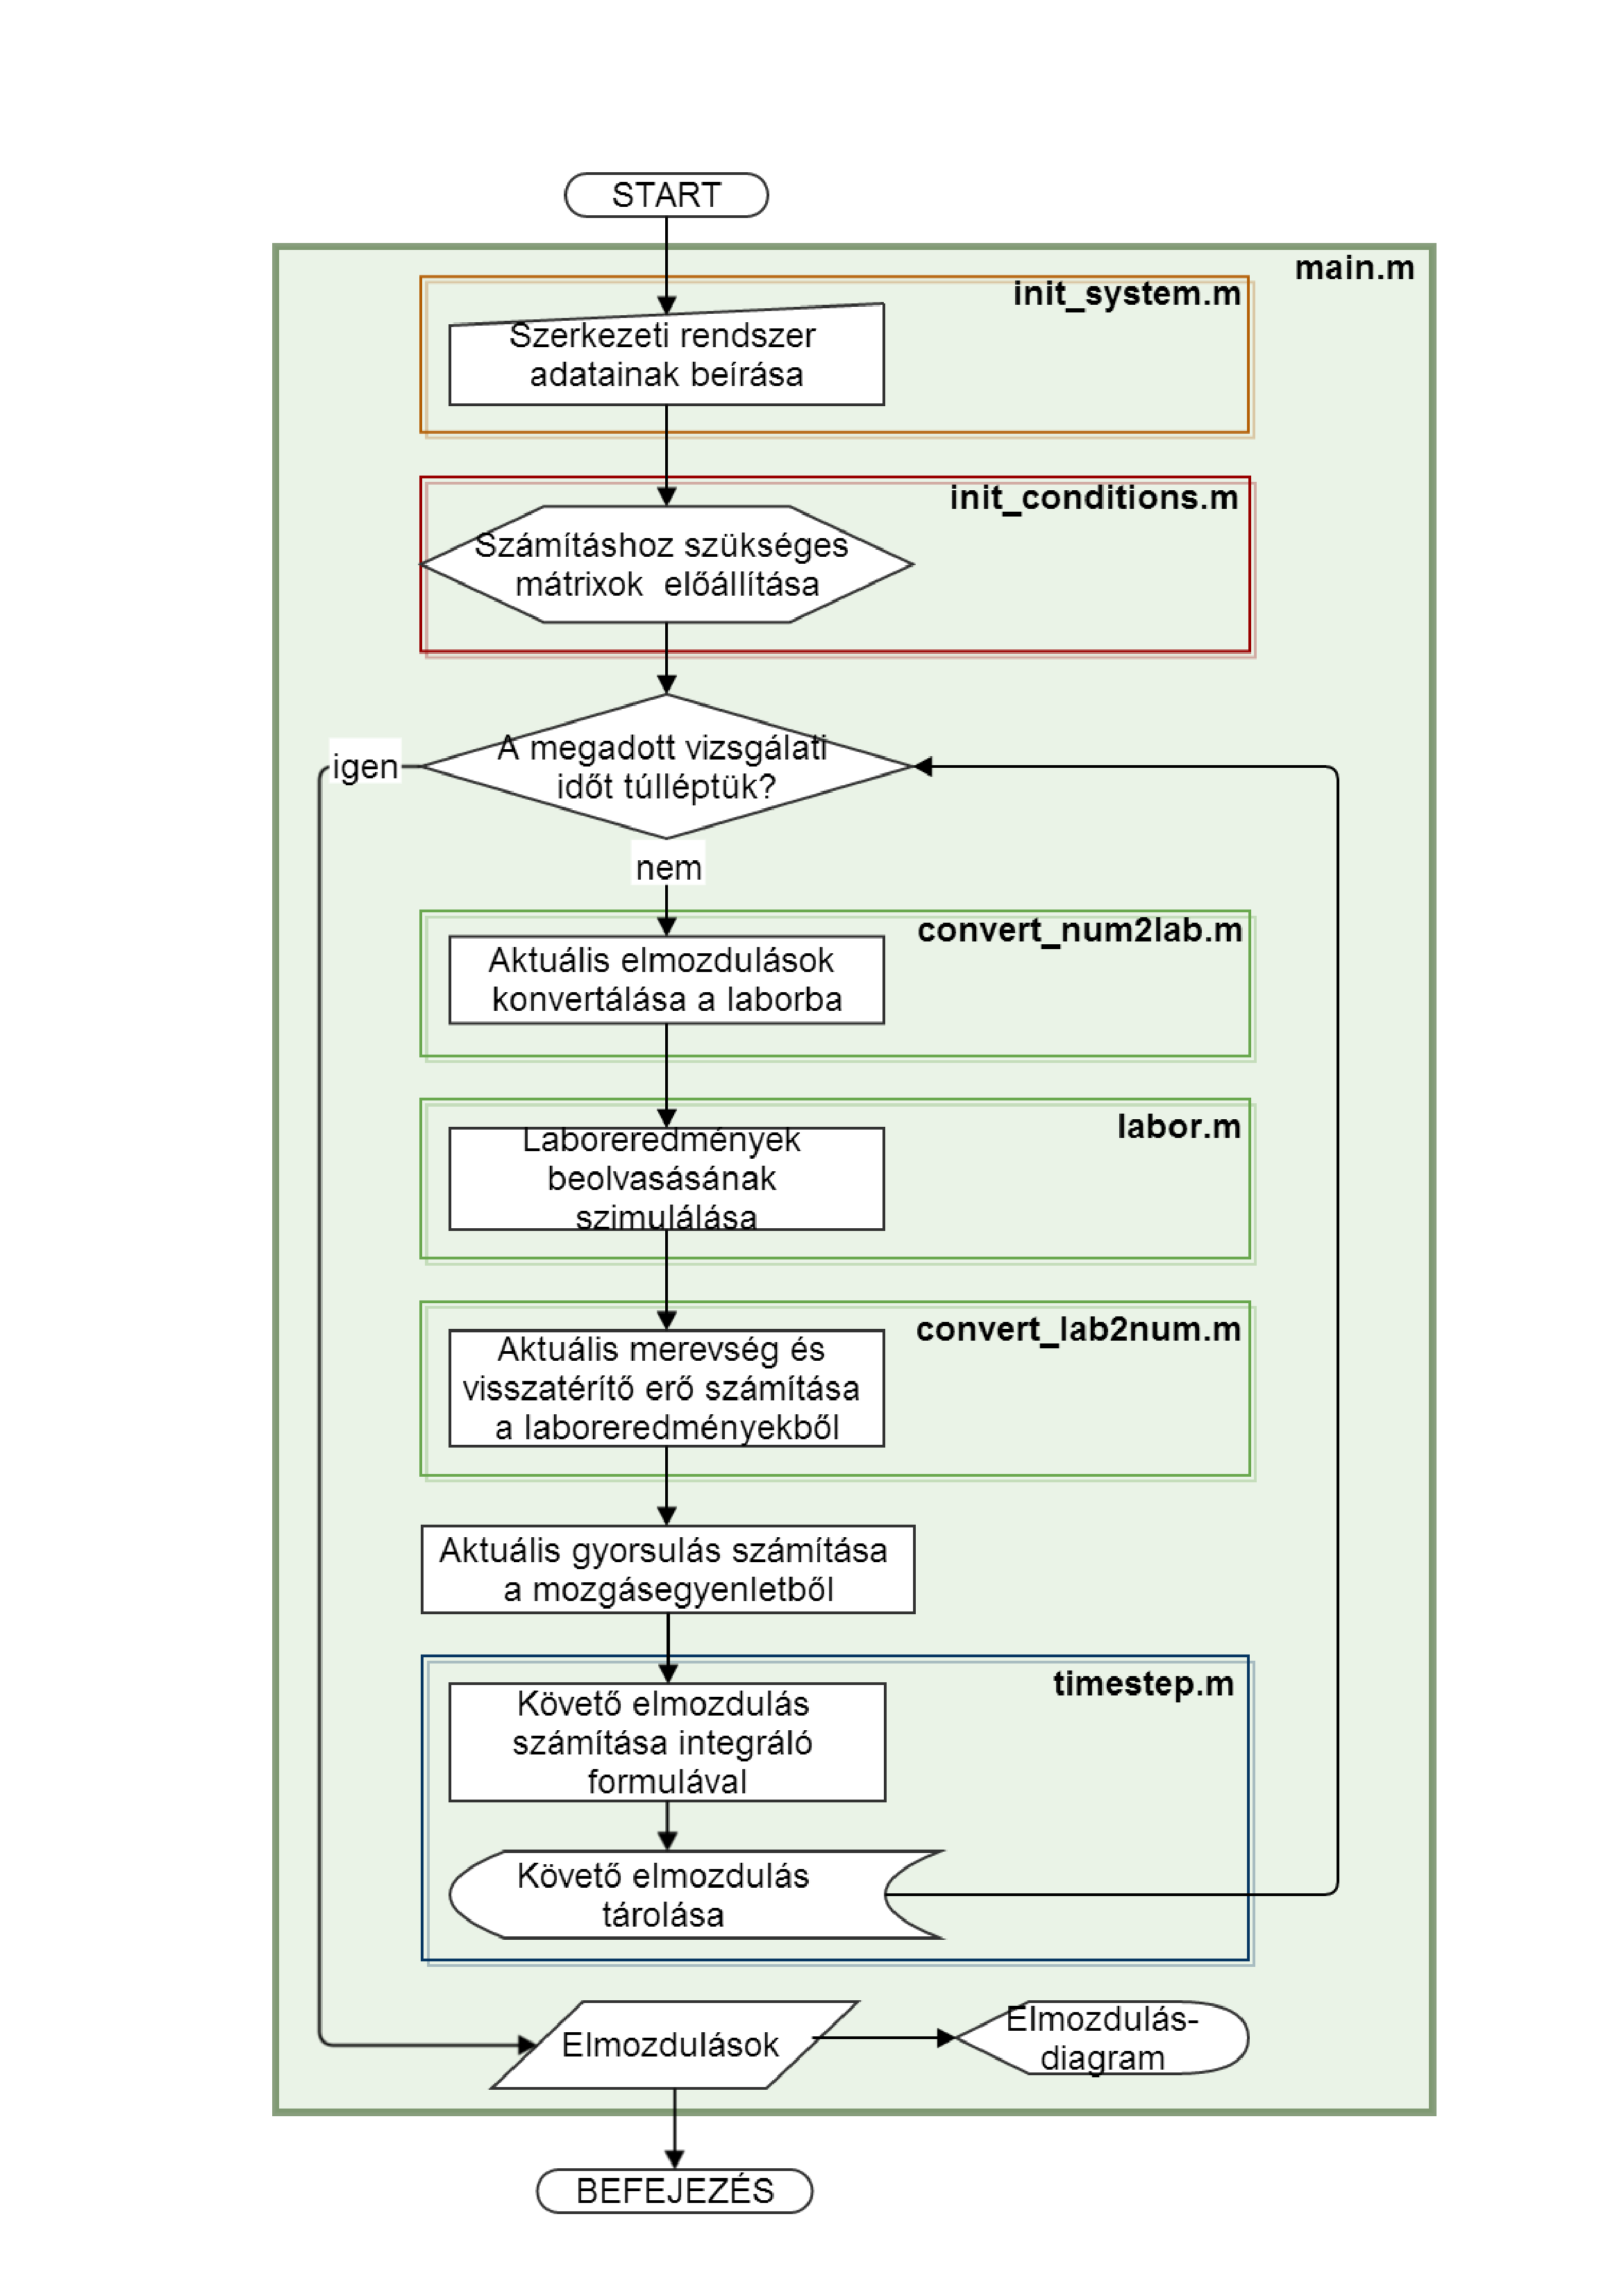
\includegraphics[trim = 0mm 5mm 0mm 40mm, clip, width=\textwidth]{hibrid_folyamatabra.pdf}
\caption{A hibrid program folyamatábrája.}
\label{fig:hibridprog_folyamatabra}
\end{figure}

A program műveleti blokkokból áll. Ezek egy része összeegyeztethető a lineáris és nemlineáris megoldóknál használtakkal. A \verb|main.m| szkript a műveleti parancssort és a beillesztett műveleti blokkokat tartalmazza. Az első lépés egy biztonsági törlés elvégzése. Ezt követően a szkript meghívja az \verb|init_system.m| fájlt, és beolvassa a vizsgált szerkezet alapadatait, majd az \verb|init_conditions.m| szkriptet hívja, ami a számítás előkészületeként a helyfoglaló és a  segédmátrixokat állítja elő. Ezt követi a kísérleti vizsgálatot és a numerikus számítást végző for ciklus. A ciklusban a \verb|convert_num2lab.m| végzi a kezdeti értékek és a numerikus számításokból adódó értékek konvertálását, a \verb|labor.m| szkript szimulálja a laboratóriumi kísérletet , a laboratóriumi kísérletekből kapott eredményeket pedig a \verb|covert_lab2num.m| fájl konvertálja a numerikus számításhoz. Ekkor az aktuális  időlépéshez tartozó gyorsulás számítása következik, majd a \verb|timestep.m| szkript elvégzi a numerikus integrálást, és elmenti az eredményül kapott, a következő időlépéshez tartozó elmozdulást. A for ciklus futása az előre megadott vizsgálati időintervallum végéig tart. Az utolsó lépés az eredmény kirajzolása egy elmozdulás - idő diagramban.

Az \verb|init_system.m| szkriptben a vizsgálat  adatait és a kezdeti feltételeket adhatjuk meg. Ezek  a vizsgálat időtartama, az időlépések nagysága, a szerkezet tömeg-, a merevségi és csillapítási mátrixa, a tehervektor, valamint a $\mathbf{u}_0$ és  $\mathbf{\dot{u}}_0$  kezdeti feltételek. Itt kell megadnunk továbbá, hogy a kísérleti próbatesten a terhelést hány lépcsőben végezzük. Ha az adott feladatban szükséges, számítjuk a szerkezet sajátkörfrekvenciáit és sajátrezgésalakjait. A csillapítási mátrix számítása is ebben a szkriptben történik. A csillapítási mátrixhoz alapvetően arányos csillapítást vesz figyelembe a program, de ezt lehet módosítani, ha a feladat megkívánja. A kezdeti feltételeken túl esetenként meg kell adni az első lépésben a labornak a  szükséges értékeket, mint a kezdeti visszatérítő erő és érintőmerevség, valamint a próbatestre alkalmazandó kezdeti elmozdulás.

Az \verb|init_conditions.m| szkript lefoglalja a helyet az elmozdulásvektoroknak, és elvégzi a számítás alatt állandó segédmátrixok előállítását és invertálását, ha szükséges. 

A \verb|convert_num2lab.m| fájl konvertálja a kezdeti feltételekből vagy a numerikus számításokból ismert aktuális elmozdulást. A program a laborban történő alkalmazáshoz szükséges geometriai összefüggéseket is itt számolja. Ehhez az \verb|U_num2lab.m| függvényt hívja meg, ami átszámolja a szerkezet globális koordináta-rendszeréből a próbatest lokális koordináta-rendszerébe az aktuális elmozdulást.

A \verb|labor.m| szkript a laborkísérletet szimulálja. Szükség esetén ezt viszonylag egyszerűen kiválthatja  a tényleges laboratóriumi vizsgálat. A  kísérletben először tároljuk az előző lépésben mért visszatérítő erőt. Az aktuális elmozdulást az \verb|init_system.m| fájlban megadott számú lépcsőben érjük el. Az utolsó előtti szakaszban mérjük az elmozduláslépcsőhöz tartozó visszatérítő erőt, majd ennek segítségével extrapolálunk az utolsó elmozduláslépcsőhöz tartozó értékre. Az elmozdulás és a visszatérítő erő változásából ekkor számíthatjuk az aktuális érintőmerevséget. A szimulált laborkísérlet annyiban különbözik a valóstól, hogy a visszatérítő erő  értékét nem mérjük, hanem számítjuk. Ehhez a \verb|resisting_force.m| függvényt hívjuk, ami a feltételezett anyagmodell alapján számítja a visszatérítő erő értékét. 

Ezt követően a laboreredményeket, az aktuális visszatérítő erőt és a próbatest aktuális érintőmerevséget konvertáljuk a numerikus számításhoz a \verb|covert_lab2num.m| szkriptben. Ekkor a próbatest lokális koordináta-rendszeréből át kell számolnunk az eredményeket a szerkezet globális koordináta-rendszerébe. Ehhez az \verb|f_s_lab2num.m| függvényt használjuk. Ha ez megtörtént, számítjuk a szerkezet aktuális merevségi mátrixát. 

A laborból konvertált adatokkal már számítható a mozgásegyenletből  az aktuális gyorsulásvektor. A \verb|timestep.m| fájl a CR algoritmus időlépéséhez tartozó lépésekkel  explicit módon számítja és tárolja a következő időponthoz tartozó elmozdulást és sebességet. Hibrid módszernél, mivel a merevségi mátrix nem állandó, az $\boldsymbol\alpha_1$
 és  $\boldsymbol\alpha_1$ integráló paramétereket is lépésenként kell számítani. 


\section{A program használatának bemutatása}\label{sec:hibr_példa}

{\ }

A hibrid szimulációs program műveleti blokkokból áll, így az egyes feladatokhoz elég néhány blokkot módosítani. Ezek általános esetben a bemeneti adatokat tartalmazó \verb|init_system.m|, valamint a globális és lokális koordináta-rendszerek közötti összefüggést meghatározó \verb|U_num2lab.m| és  \verb|f_s_lab2num.m| fájlok.  A vizsgált szerkezet paramétereit, a merevségi és tömegmátrixokat, a csillapítási mátrix előállatásának módját, a szerkezetre ható terhelést és a kezdeti feltételeket, illetve a labornak küldött kezdeti értékeket mind az \verb|init_system.m| szkriptben módosíthatjuk. A szerkezet geometriája alapján a globális koordináta-rendszer és a próbatest lokális koordináta-rendszere közötti átszámítás képleteit  az \verb|U_num2lab.m| és az \verb|f_s_lab2num.m| függvényekben adhatjuk meg. 

Szimulált hibrid szimuláció esetében megválaszthatjuk továbbá, hogy milyen anyagmodellt veszünk figyelembe a nemlineáris viselkedésű próbatestnél.  Az anyagmodell számítását a \verb|resisting_force.m| függvényben adhatjuk meg, mivel annak változása  a visszatérítő erőben jelenik meg.

A szimulált kísérletről a valós kísérleti eljárásra való áttéréshez a \verb|labor.m| szkriptben számított aktuális visszatérítő erő és érintőmerevség helyett  a laboratóriumi kísérletben mért értékeket használjuk. Ehhez a \verb|labor.m| fájlt ki kell cserélni egy olyan  szkriptre, ami ezeket az értékeket beolvassa.

\begin{figure}[h!]
\centering
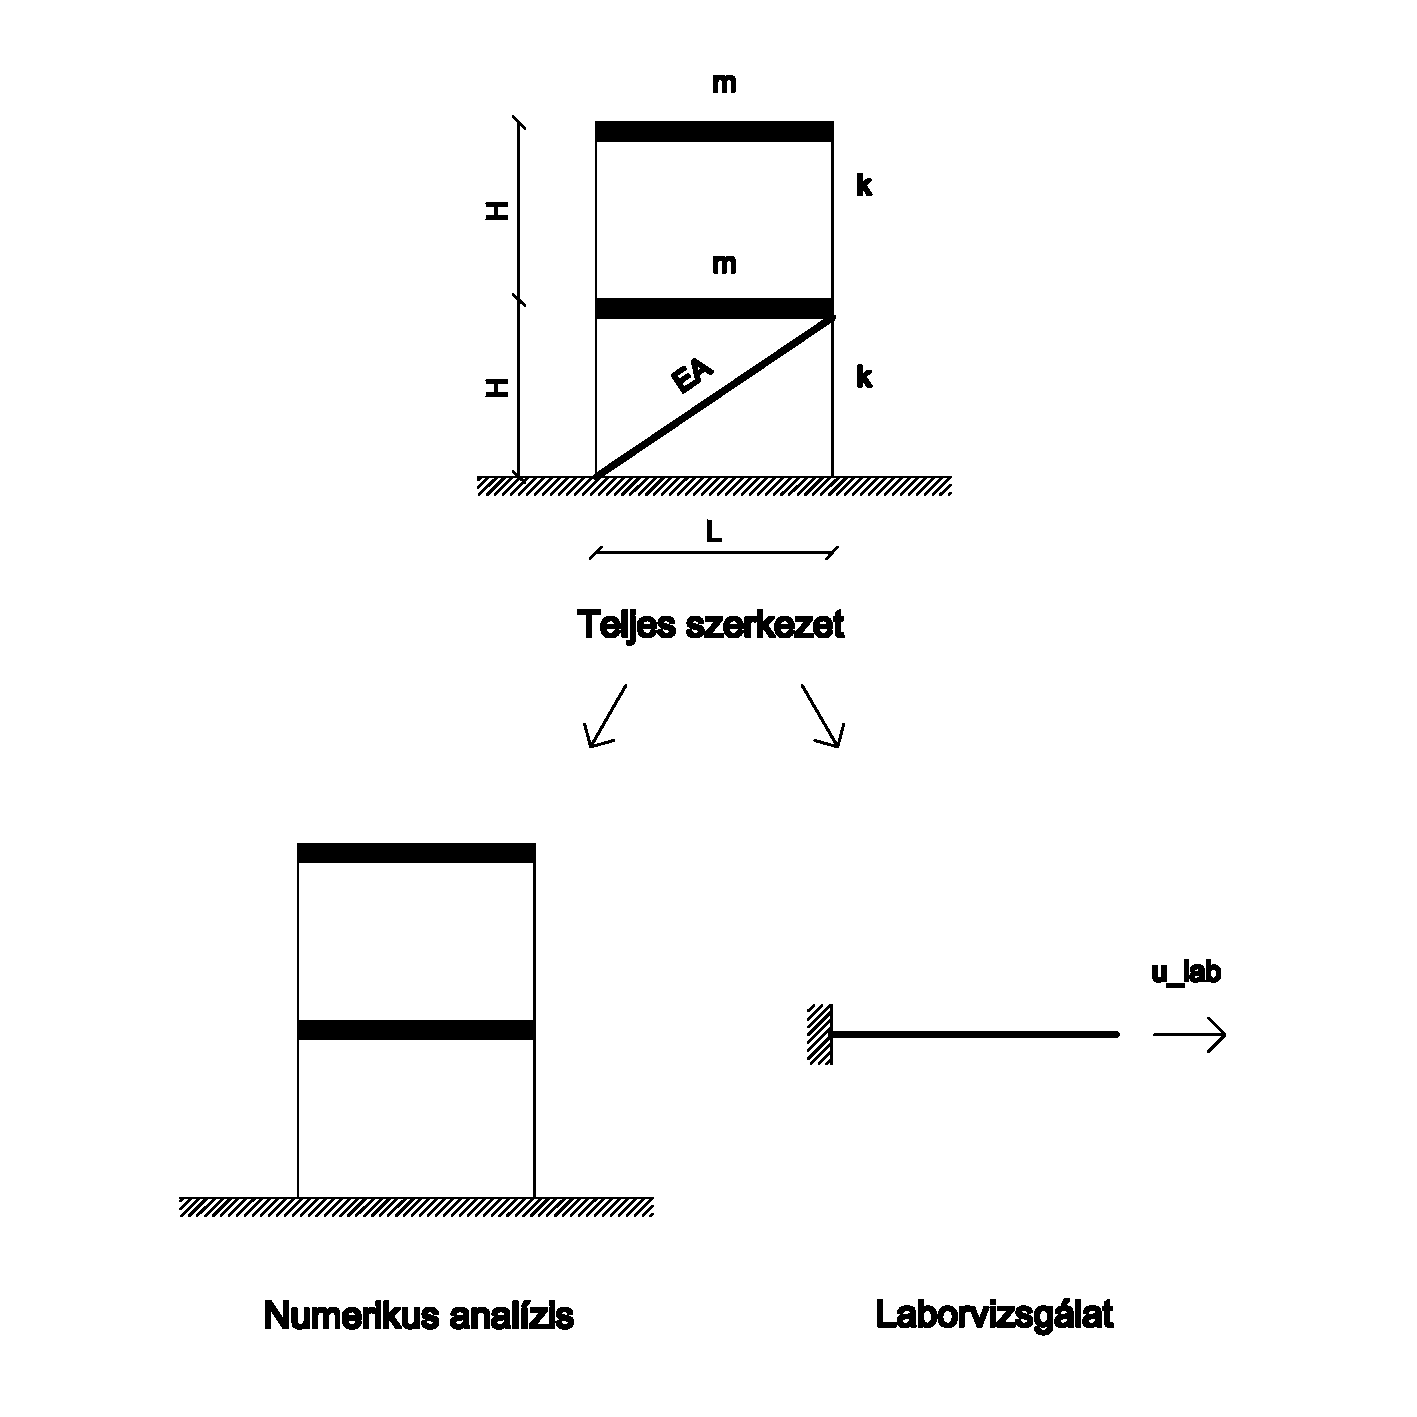
\includegraphics[ width=0.8\textwidth]{hidrid_abra.pdf}
\caption{A hibrid szimulációs programmal vizsgált szerkezet  és szétbontása.}
\label{fig:hibridprogpélda}
\end{figure}


A program használatát egy konkrét példán mutatom be. Adott a \ref{fig:hibridprogpélda} ábrán látható kétszintes keret, az alsó szinten egy ferde, nemlineáris viselkedésű merevítő rúddal. A rendszer modellezését a \ref{fig:viselkedési modell} ábrán láthatjuk. A feladatban a merevítő rúd viselkedését  szimulált laborkísérlettel, a  szerkezet többi részét pedig numerikusan vizsgáljuk. A szerkezet fesztávolsága és a szintek magassága egyaránt $3 m$. Az egyes szintek tömege $m = 45 t$, a szintenkénti merevség $k = 18000 kN/m$. A merevítő rúd merevsége $EA = 76367 kN$.  Modellezésére a \ref{subsec:nemlinstat} pontban a nemlineáris programnál bemutatott nemlineárisan rugalmas anyagmodellt használjuk, és a rúd megnyúlását pontosan számítjuk. Ezzel egy geometriai és egy anyagi nemlinearitást is figyelembe veszünk. A  szerkezeten arányos csillapítást alkalmazunk, $\alpha$ és $\beta$ értékét úgy vesszük fel, hogy mindkét módban $\xi$ tényező értéke $5\%$ legyen.   A kezdeti feltételek,  a laborvizsgálathoz szükséges  kezdeti visszatérítő erő és érintőmerevség, valamint a próbaestre alkalmazandó kezdeti elmozdulás értéke zérus.

\begin{figure}[h!]
\centering
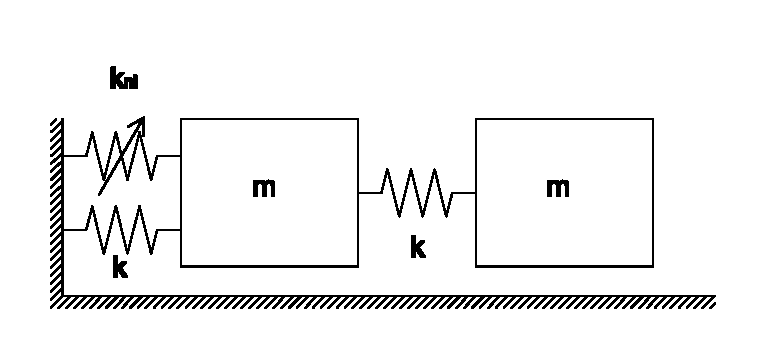
\includegraphics[ width=0.6\textwidth]{nemlin_modell.pdf}
\caption{A hibrid szimulációs programmal vizsgált szerkezet modellezése.}
\label{fig:viselkedési modell}
\end{figure}

A szerkezetet adatai képletekkel:
\begin{align*}
  & L = 3 m  & & H = 3 m   & \\
  & EA = 76367 kN & k_n = \frac{EA}{\sqrt{L^2+H^2}} & \\
  & \mathbf{M}  = \left[\begin{array}{rr}  45 & 0 \\ 0 & 45 \end{array} \right]t   &  & \mathbf{K} = 18000\left[\begin{array}{rr} 2 & -1 \\ -1 & 1 \end{array} \right]\frac{kN}{m}  &  \\
  & \mathbf{C}  = \alpha\mathbf{M}+\beta\mathbf{K}  &  & \xi = 0,05  & \\
  & \mathbf{u}(0)  = \left[\begin{array}{c} 0 \\ 0 \end{array} \right]  & & \mathbf{\dot{u}}(0) = \left[\begin{array}{c} 0 \\ 0 \end{array} \right] & \\
  & f_{s,lab,0} = 0 kN & &U_{lab,0} = 0 m   & \\
  & k_{t,lab,0} = k_n  & & f_s(\Delta{l})  = a \arctan{b\Delta{l}}&
  \end{align*}

Ezek alapján  az \verb|init_system.m| fájl a következő:

 \lstinputlisting{"MATLAB/hibrid/init_system.m"}
 
 
 A szerkezet geometrája alapján a globális és lokális koordináta-rendszerek közötti átszámítást leíró \verb|U_num2lab.m| és \verb|f_s_lab2num.m| függvények:
 
 \lstinputlisting{"MATLAB/hibrid/U_num2lab.m"}
 \lstinputlisting{"MATLAB/hibrid/f_s_lab2num.m"}


 A  \verb|resisting_force.m| függvény a szerkezet anyagmodellje alapján a következő:
 
  \lstinputlisting{"MATLAB/hibrid/resisting_force.m"}
 
  
  A példán keresztül látható, hogy a szerkezet bemeneti adatainak megadására szolgáló fájlok elkülönülnek a számítást végző műveleti blokkoktól, így a program módosítása az egyes feladatokhoz viszonylag egyszerűen elvégezhető. 
  
  
\section{Hibrid szimulációs program verifikálása}\label{sec: hibrid ver.}

{\ }

A következőkben a hibrid szimulációs program verifikálását végzem el a \ref{sec:hibr_példa} alfejezetben bemutatott kétszintes merevített kereten. A vizsgálati eredményeket ugyanazon a szerkezeten végzett nemlineáris számítás eredményeivel hasonlítom össze.


\subsection{Kijelölt szerkezet vizsgálata hibrid szimulációval}\label{subsec:71_hibrid}

{\ }

A szerkezetre teherként az El Centro földrengés gyorsulásaiból számított földrengésterhet működtetem.  A földrengés a valóságban már lezajlott 1940-ben  Kalifornia államban. Az El Centro-t gyakran alkalmazzák a földrengésszámítások során.  A \ref{fig:ec gyors}  ábrán az El Centro földrengés gyorsulásai  láthatók az idő függvényében. Az adatok a Vibrationdata  \cite{elcentro} honlapjáról származnak.

\begin{figure}[h!]
\centering
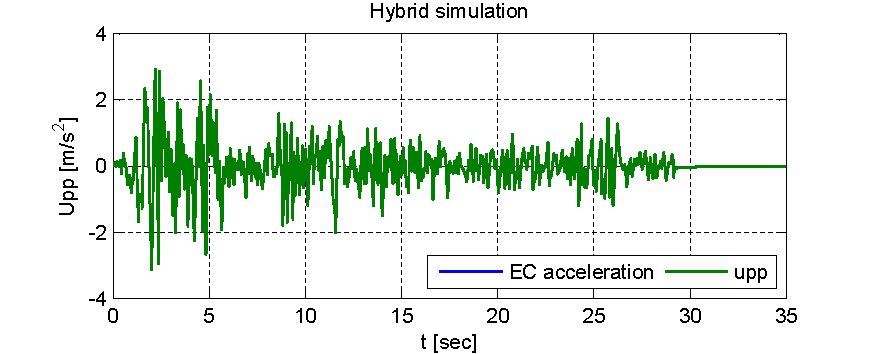
\includegraphics[width=\textwidth]{72_gyorulas_EC.pdf}
\caption{Az El Centro földrengés gyorsulásai.}
\label{fig:ec gyors}
\end{figure}

Az El Centro gyorsulásadatait  a programba az \verb|EQ_load.m| függvénnyel töltöm be. A függvény a  gyorsulásadatok beolvasását  és a vizsgált diszkrét időpontbeli értékek interpolálását végzi el.  A függvény a Függelék \ref{chap: függ hibrid prog}. pontjában látható. 

A tehervektor számítása a gyorsulásokból a \eqref{támrezg1} támaszrezgés  egyenletéből adódik:

\begin{equation}
 \mathbf{q} = -\mathbf{M}\mathbf{\ddot{u}}_g(t)
\end{equation} 

Az \verb|init_system.m| fájlban a tehervektor megadása  a következőképpen alakul:
 \lstinputlisting[firstline=53, lastline=66]{"MATLAB/hibrid_72/init_system.m"}
 
A szimulációból kapott elmozdulásokat az idő függvényében a \ref{fig:ec_elm-a} ábrán láthatjuk.


\subsection{Kijelölt szerkezet vizsgálata nemlineáris analízissel}

{\ }

A nemlineáris programban ugyanazt a \ref{fig:hibridprogpélda} ábrán látható kétszintes keretet számoltuk. Az elmozdulásokat a Newmark módszer elmozdulásos változatával számoltuk. A szerkezetre a nemlineáris programban is az El Centro-t működtetem. A gyorsulásadatok betöltését ugyanúgy az \verb|EQ_load.m| függvénnyel végeztem. Az \verb|init_system.m| szkriptben csak a kezdeti feltételek megadása különbözik a hibrid szimulációnál látottaktól:

 \lstinputlisting[firstline=69, lastline=84]{"MATLAB/nonlinear_system_71/init_system.m"}

A nemlineáris merevítő rúd  anyagmodellje megegyezik a hibrid számításnál alkalmazottal, így ugyanazt a geometriai és anyagi nemlinearitást vesszük figyelembe. Ez alapján programban a visszatérítő erő számítása a \verb|resisting_force.m| és az érintőmerevségé a \verb|tangent_stiffness.m| függvényekben a következő:

\lstinputlisting{"MATLAB/nonlinear_system_71/resisting_force.m"}
\lstinputlisting{"MATLAB/nonlinear_system_71/tangent_stiffness.m"}


\subsection{A nemlineáris és a hibrid szimulációs program eredményeinek összehasonlítása}

{\ }

A feladat hibrid és nemlineáris számításából a \ref{fig:ec_elm-a} és \ref{fig:ec_elm-b} ábrákat összehasonlítva szemre hasonló eredményeket kaptunk. A két ábra között igazán nincs  különbség,  ha egymás fölé vetítjük ezeket, akkor is csak minimális  eltérés figyelhető meg. 

\begin{figure}[h!]%
\centering
\subfigure[][]{%
\label{fig:ec_elm-a}%
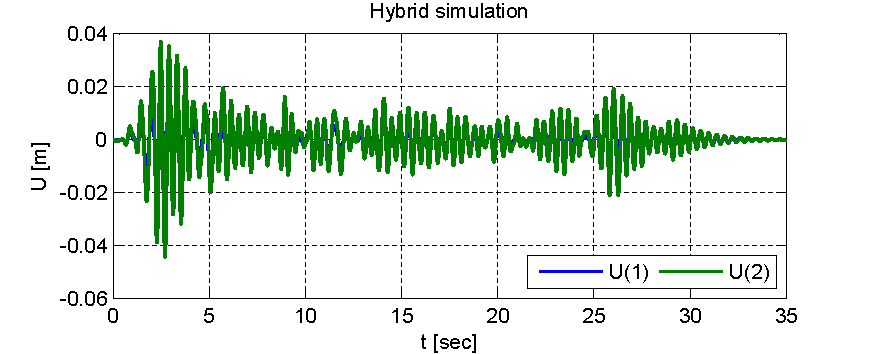
\includegraphics[width=\textwidth]{72_elmozdulas.pdf}}%
\\
\subfigure[][]{%
\label{fig:ec_elm-b}%
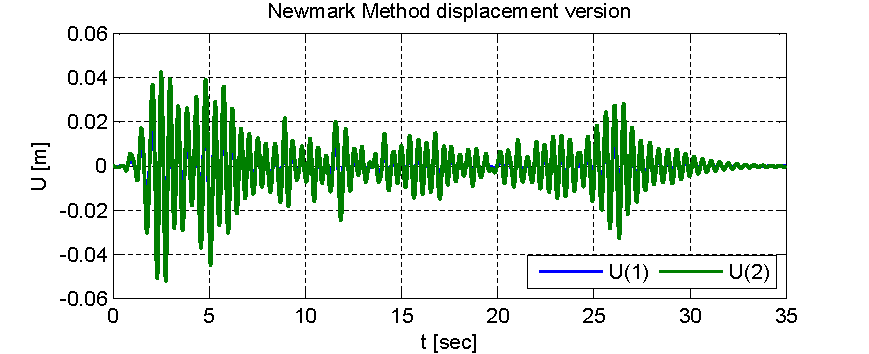
\includegraphics[width=\textwidth]{71_elmozdulas.pdf}}%
\caption[Kétszintes merevített keret elmozdulásai.]{Kétszintes merevített keret elmozdulásai az El Centro földrengés hatására:
\subref{fig:ec_elm-a} hibrid szimulációval;
\subref{fig:ec_elm-b} nemlineáris számítással.}%
\label{fig:ec_elm}%
\end{figure}

Azonban méretezési feladatokban  nem annyira az időbeni lefutás fontos, hanem az eredmények  maximum (abszolút)értékei, ezért kiválogattam ezeket, és összegyűjtöttem a \ref{7_table} táblázatba. Fontos megjegyezni, hogy ezek tényleges értékek, nem pedig a modálanalízis egyes eredményeinek valamilyen közelítésen alapuló összegzése. 
A táblázatból látszik, hogy a számítások között minimális a különbség. A maximális elmozdulások között az eltérés nagyságrendileg néhány milliméter.

\begin{table}[h!]
\centering
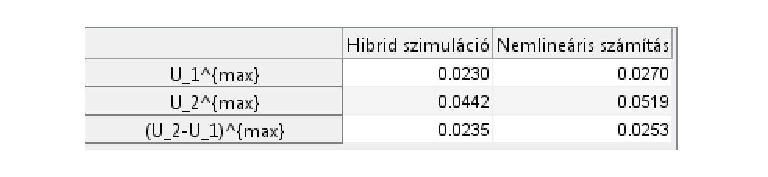
\includegraphics[width=0.7\textwidth]{7_table.pdf}
\caption{A hibrid és a nemlineáris programmal számított maximális elmozdulások.}
\label{7_table}
\end{table}


\chapter[Hibrid szimulációs program alkalmazása]{Hibrid szimulációs program alkalmazása szeizmikus szigeteléssel ellátott szerkezeten}\label{chap: hibrid alk}

\section {Szeizmikus szigetelés}

{\ }

A földrengésekből adódó károsodások kockázatának csökkentésére különféle technológiák léteznek. A hagyományos megerősítési módok mellett megjelentek a  rezgést csökkentő és elszigetelő szerkezeti rendszerek. Az aktív kontroll rendszereknél (Active Control System - ACS) olyan számítógép vezérlésű lengés-kiegyensúlyozó szerkezetet építenek be, ami külső energia  hatására végez munkát (pl. változtatják a szerkezet merevségét a lökésekkel összhangban). A passzív kontroll rendszerek (Passive Control Systems - PCS) esetében  olyan szerkezetek beépítése történik, amelyek hatással vannak az építmény rezgés-jellemzőire. Léteznek hibrid kontroll rendszerek is ( Hybrid Control Systems - HCS), ahol ACS és PCS rendszereket kombinálnak. Szél és kisebb földrengések esetén PCS rendszerként, nagyobb amplitúdójú dinamikus terhelésnél pedig az ACS rendszerként viselkednek. 

A leggyakrabban használt rendszerek ezek közül a passzív kontroll rendszerek. Ha az építménybe PCS rendszert építenek be elérhető, hogy a  szerkezet és a földrengés periódusa elkülönüljön, így elkerülhető a rezonancia jelensége. A PCS rendszerek két osztályba sorolhatók: szeizmikus szigetelők (Base Isolators) és lengéscsillapítók (Energy Dampers). Ezek közül a továbbiakban a szeizmikus szigetelést mutatom be. 

A szeizmikus szigetelések beépítése viszonylag új technológia. Az első elméletek körülbelül száz éve jelentek meg, azonban  csak a '70-es évek óta  kutatják. Bár csak néhány évtizede vált kivitelezhetővé, mégis rendkívül  elterjedt az alkalmazása.

 A szeizmikus szigetelő rendszerek különösen nagy  jelentősséggel bírnak a már meglévő szerkezetek megerősítésénél, mivel ezeknél a bizonytalan anyagjellemzők és merevségi viszonyok körülményessé  teszik a hagyományos megerősítési módok alkalmazását. Ezekben az esetekben a szeizmikus szigetelés utólagos beépítése megoldást jelent a problémára.
 
 A már meglévő épületek szeizmikus teher elleni megerősítésére több esetben is szükség lehet:
 \begin{itemize}
 \item a kiemelt jelentősségű épületeknél, mint kórházak, mentőállomások, telefonközpontok
 \item műemlék jellegű épületeknél
 \item hidaknál
 \item nagy kihasználtságú épületek, irodaházak, szállodák esetében
 \item veszélyes ipari létesítményeknél, beleértve a víz- és benzintartályokat, atomreaktorokat
 \end{itemize}
 


Szeizmikus szigetelések beépítésénél \cite{simon vigh}  célunk nem a kritikus elemek teherbírásának növelése, hanem a szerkezet válaszának módosításával, energiaelnyeléssel, csillapítással, az igénybevételek és az épületre jutó szeizmikus hatások csökkentése .  
A szeizmikus szigetelőket az alépítmény és a felépítmény közé építik be, mereven rögzítve. Vízszintes merevségük kicsi, ezért a domináns  szeizmikus erők hatása a szerkezetre jelentősen csökken. Az energiát súrlódás vagy hiszterézis viselkedés útján nyelik el. A \ref{fig:szig} ábrán a szeizmikus szigetelés alapelve látható.

\begin{figure}[h!]
\centering
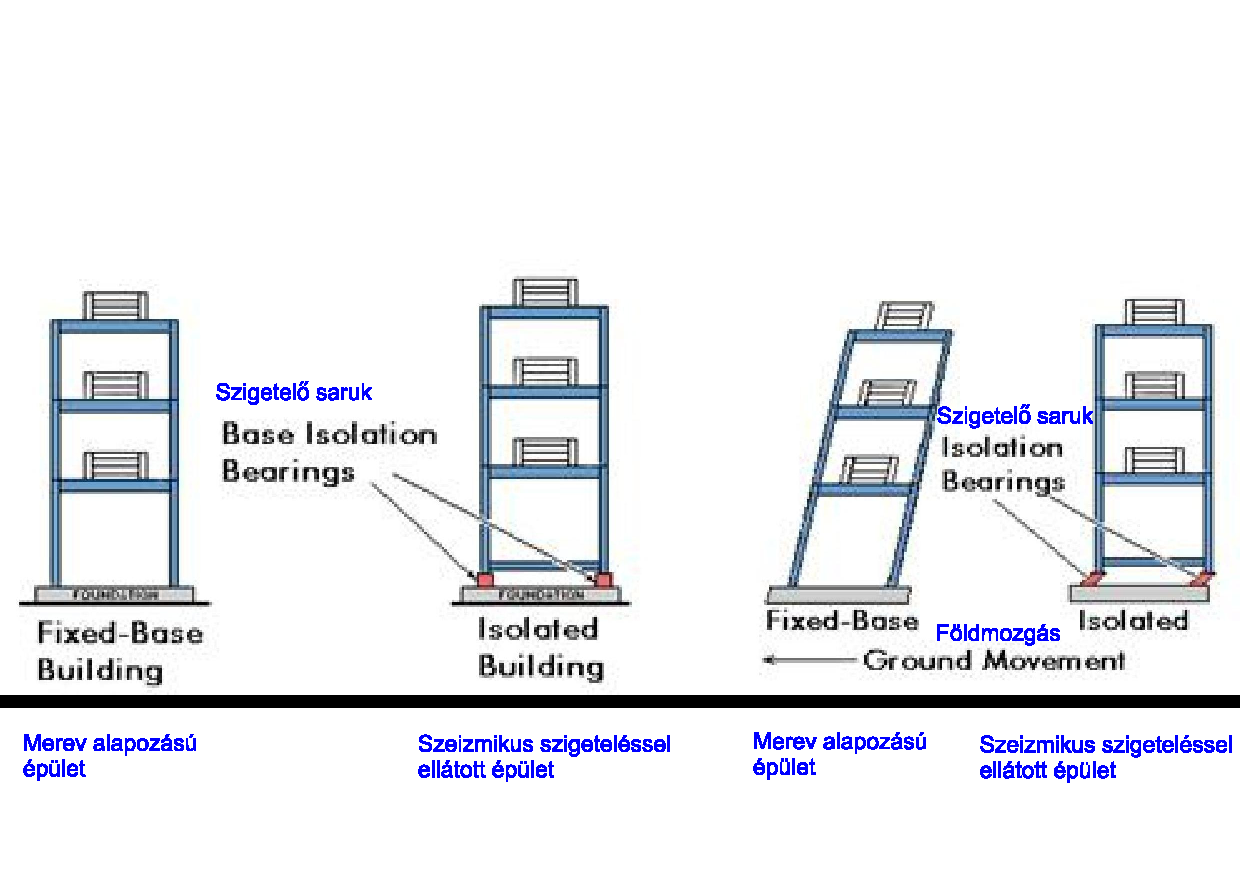
\includegraphics[trim = 0mm 15mm 0mm 25mm, clip, width=0.8\textwidth]{base_isolation.pdf}
\caption{A szeizmikus szigetelés alapelve \cite{hibrid wiki}.}
\label{fig:szig}
\end{figure}

 

Az EN 15129 \cite{antiizé} szerint a szeizmikus szigetelőket  a következőképpen csoportosíthatjuk:
\begin{itemize}
\item elasztomer saru
\item ólom- vagy acélmagos gumi saru
\item egyenes felszínű csúszó saru
\item görbe felszínű csúszó saru
\end{itemize}

Az elasztomer szigetelő saruk természetes vagy  szintetikus gumiból készülnek hengerelt  acéllemezekkel erősítve. Általában rugalmas viselkedésűek. A külső behatásokkal szemben, mint az UV sugárzás, a szerkezet védelméről gondoskodni kell. A berendezések csillapítási mértéke 6-20\% között mozoghat. 
 
A merevítő maggal ellátott gumi saru (Lead Rubber  Bearing -  LRB) az egyszerű elasztomer sarutól annyiban különbözik, hogy a saru belsejében egy acél- vagy ólommag kerül elhelyezésre. Az elhelyezett mag nagyobb vízszintes terhek felvételére képes, így a saru vízszintes irányban merevebbé válik, hiszterézis viselkedése viszont jóval kedvezőbb lesz. A csillapítási mértéke elérheti akár a  40\%-ot is.
 
A csúszólapos saruknál az energiaelnyelés súrlódással történik. A  maximális csillapítási mérték 5-35\% között mozog. Kialakítás szempontjából két fajtájuk van. A  lapos csúszófelülettel kialakított saruk (sliding isolators) hátránya, hogy képtelenek újraközpontosítani (recentering) önmagukat és a felépítményt a terhelés után, erre külön rugalmas elemeket kell beépíteni. A görbe felületű csúszólapos sarunál ezzel ellentétben a konkáv felületnek köszönhetően a vízszintes mozgás  függőlegessel jár együtt. Ezért terhelés közben  a potenciális energia megnő, ami arra készteti a sarut, hogy visszatérjen eredeti, kisebb potenciállal rendelkező helyzetébe. 
  
 
\begin{figure}[h!]
\centering
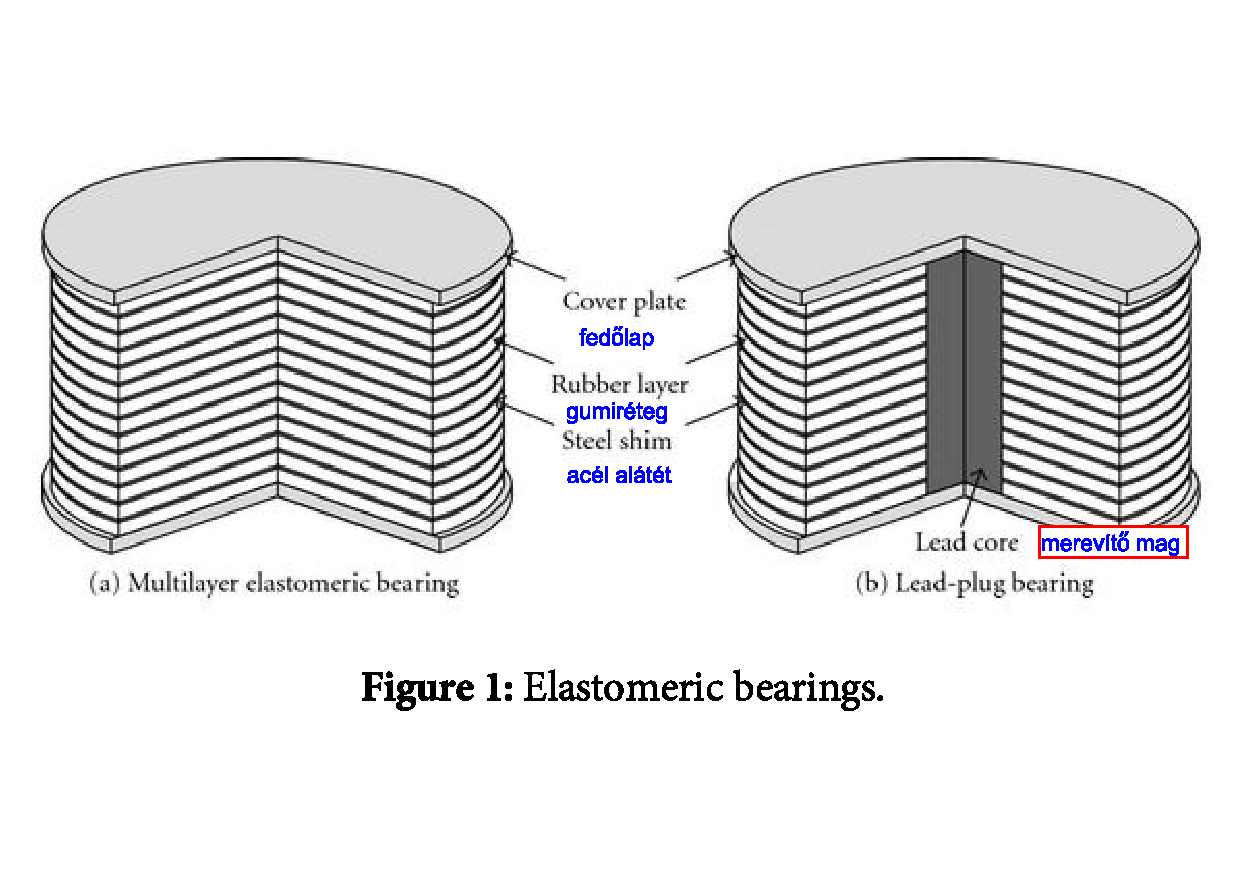
\includegraphics[trim = 0mm 53mm 0mm 15mm, clip, width=0.85\textwidth]{Assessment.pdf}
\caption{Egyszerű és merevítő maggal ellátott elasztomer saru \cite{rubber}.}
\label{fig:linprog}
\end{figure}
 
A szeizmikus szigeteléssel utólag ellátott épületek között az első a Salt Lake City-ben található Város- és Megyeháza volt. A munkálatokat 1989-ben végezték, egyszerű és merevített elasztomer sarukat építettek be. A híres szeizmikus szigeteléssel ellátott épületek között  szerepel a Dél Kaliforniai Egyetem Oktató Kórháza is, amit a merevített gumi szigetelő saruk sikeresen megvédtek az  1994-es Los Angeles-i földrengésben.
 
A következőkben bemutatom a szeizmikus szigetelés csillapító hatását egy konkrét példán keresztül. A szerkezetet összehasonlítom a nem elválasztott szerkezet viselkedésével.
% \url{ http://eda.eme.ro/bitstream/handle/10598/14508/02_FMTU1997%20_%20Gabor%20Aron%20_%20221-224%20old.pdf?sequence=1} }

\section{Szeizmikus szigetelés  csillapító hatásának vizsgálata}

{\ }

A szeizmikus szigetelés csillapító hatását a Chopra könyv \cite{chopra} 23.4.1. pontjában bemutatott ötszintes épületen vizsgáltam  úgy, hogy összehasonlítottam ugyanannak  a szerkezetnek a viselkedését fix megtámasztással és  izoláltan.  A  fix megtámasztású szerkezet elmozdulásait   a \ref{subsec: lin prog szerk} pontban bemutatott  lineáris megoldó programban számítottam,  a szeizmikus szigeteléssel ellátott szerkezetet pedig vizsgáltam a lineáris megoldó programban, illetve a \ref{chap: hibrid progi}. fejezetben ismertetett szimulált hibrid szimulációs programban is. A lineáris megoldó programban  a szigetelés egy lineárisan rugalmas anyagmodellt követ. A hibrid programban egy lineárisan rugalmas - lineárisan felkeményedő képlékeny anyagmodellt alkalmaztam.  A szerkezet többi részét mindhárom esetben lineárisnak feltételeztük. A számításokat ezúttal metrikus rendszerben végeztem.


\begin{figure}%
\centering
\subfigure[][]{%
\label{fig:8rajz-a}%
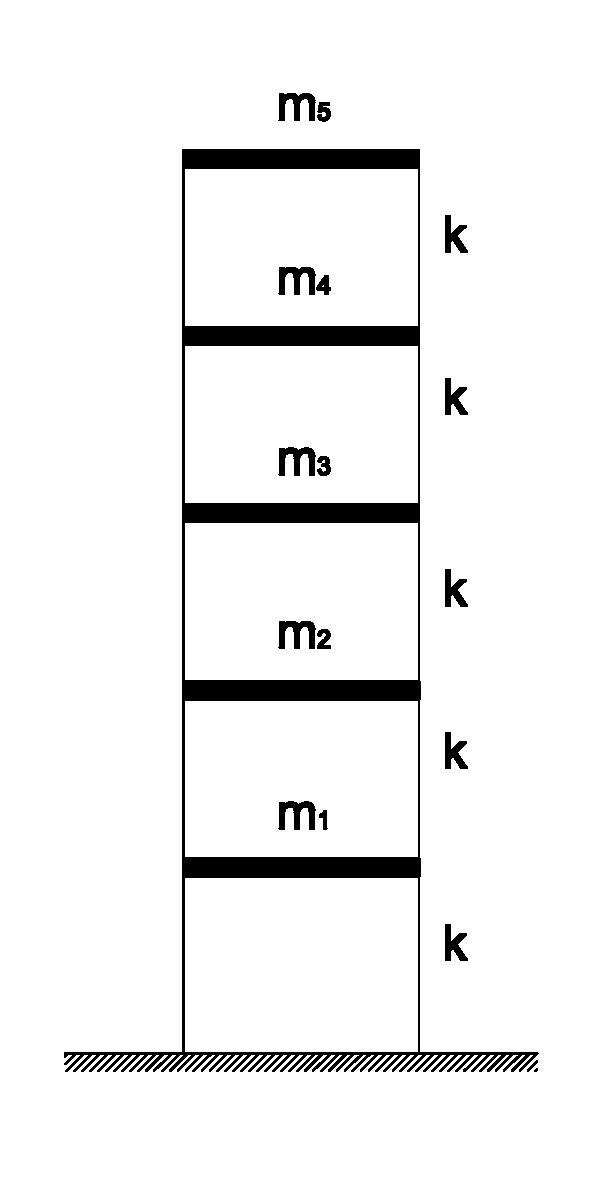
\includegraphics[width=0.3\textwidth]{fix.pdf}}%
\hspace{8pt}%
\subfigure[][]{%
\label{fig:8rajz-b}%
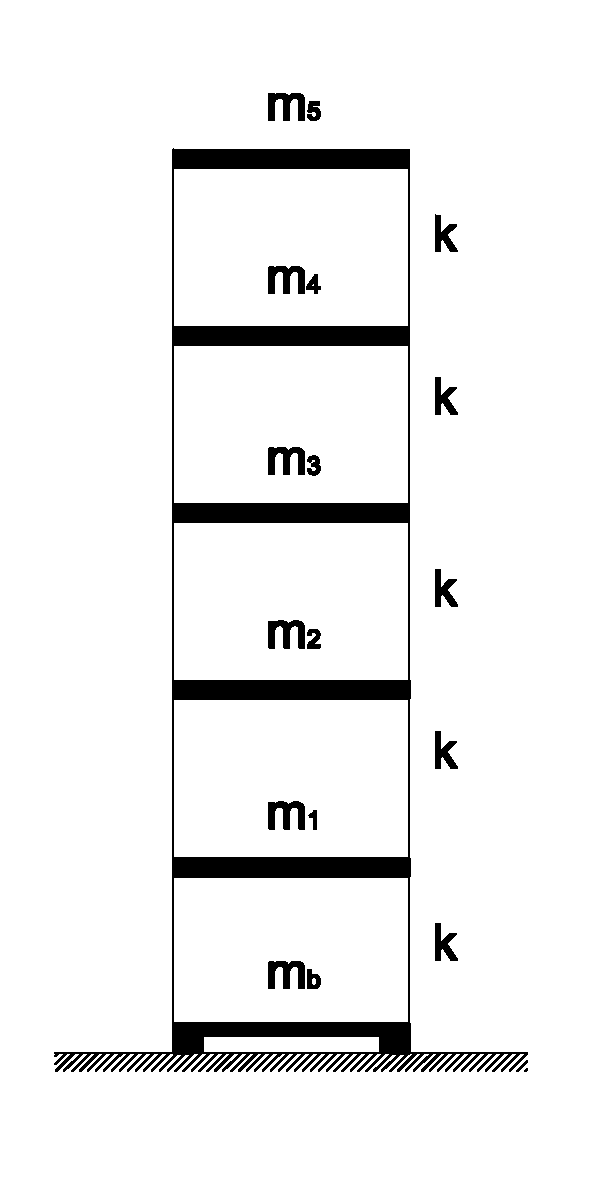
\includegraphics[width=0.3\textwidth]{base.pdf}}%
\caption[A \cite{chopra} 23.4.1 feladatban vizsgált ötszintes keretek.]{A \cite{chopra} 23.4.1 feladatban vizsgált ötszintes keretek: 
\subref{fig:8rajz-a} fix megtámasztású szerkezet;
\subref{fig:8rajz-b} szeizmikus szigeteléssel ellátott szerkezet.}
 \label{fig:8rajz}%
\end{figure}


A szerkezetre mindhárom esetben az El Centro földrengésterhet működtettem. Ennek számítása megegyezik a \ref{subsec:71_hibrid} pontban ismertetettel.


\subsection{Fix megtámasztású szerkezet  lineáris vizsgálata}

{\ }

A fix megtámasztású idealizált szerkezet  a \ref{fig:8rajz-a} ábrán látható. A szerkezetet $\mathbf{M}_{fix}$ tömegmátrix, a $\mathbf{K}_{fix}$ merevségi és $\mathbf{C}_{fix}$ csillapítási mátrixok határozzák meg. Az egyes szintek tömege $m = 100 kips/g = 45,359 t$,  $k$ merevségüket pedig úgy választjuk meg, hogy  a sajátrezgésidő $T_{1,fix} = 0.4 sec$. A szerkezet csillapítását a klasszikus formulával számoljuk, az n-edik szinten $\xi_{fix,n}$ csillapítási tényezővel. A klasszikus csillapítási mátrix $\mathbf{C}_{fix} = \alpha_1\mathbf{K}_{fix}$, $\alpha_1$ értékét $\xi = 2\%$  csillapítási tényezővel számolva.  

A szerkezetet leíró mátrixok számítása:
\begin{align*}
  & \mathbf{M}_{fix}  = m\left[\begin{array}{rrrrr}  1 & 0 & 0 & 0 & 0  \\ 0 & 1 & 0 & 0 & 0 \\ 0 & 0 & 1 & 0 & 0 \\ 0 & 0 & 0 & 1 & 0 \\ 0 & 0 & 0 & 0 & 1  \end{array} \right] t   &  & \mathbf{K}_{fix} = k \left[\begin{array}{rrrrr} 2 & -1 & 0 & 0 & 0  \\ -1 & 2 & -1 & 0 & 0 \\ 0 & -1 &2 & -1 & 0 \\ 0 & 0 & -1 & 2 & -1 \\ 0 & 0 & 0 & -1 & 1 \end{array} \right]\frac{kN}{m}  &  \\
  & \mathbf{C}_{fix}  = \alpha_K\mathbf{K}_{fix}  &  & \alpha_K = \frac{\xi}{\sqrt{\omega_1}} & \\
  & \xi_{fix,n} = \alpha_K\sqrt{\omega_n}& & T_{fix,n} = \frac{2\pi}{\sqrt{\omega_n}} &  
\end{align*} 

\lstinputlisting[firstline=29, lastline=51]{"MATLAB/linear_system_8_fix/init_system.m"}
\lstinputlisting[firstline=74, lastline=89]{"MATLAB/linear_system_8_fix/init_system.m"}

A fix megtámasztású szerkezet első szintjének abszolút (illetve ebben az esetben relatívnak is tekinthető) és tetőponti elmozdulásai a \ref{fig:8_linfix} ábrán láthatók.



\subsection{Szeizmikus szigeteléssel ellátott szerkezet lineáris vizsgálata}

{\ }

A szeizmikus szigeteléssel ellátott épület idealizált modelljét a \ref{fig:8rajz-b} ábra mutatja. A szigetelő szerkezet jellemzésére bevezetjük a következő összefüggéseket:
\begin{subequations}
\label{eq:tb}
\begin{align}
& T_b = \frac{2\pi}{\omega_b}, &  & \omega_b = \sqrt{\frac{k_b}{\mathbf{M}_{fix}+m_b}}; & \\
& \xi_b = \frac{c_b}{2(\mathbf{M}_{fix}+m_b)\omega_b}.&
\end{align}
\end{subequations}

A $T_b$ értéket értelmezhetjük a szigetelő rendszer sajátrezgésidejeként, és $\xi_b$-t a csillapítási tényezőjeként. Ahhoz, hogy a szeizmikus szigetelés hatékonyan csökkentse az épületben a földrengés által kiváltott erőket, $T_b$-nek sokkal hosszabbnak kell lennie, mint $T_{1,fix}$-nek, a merev alátámasztású épület sajátrezgésidejének. Az N emeletes szeizmikus szigeteléssel ellátott szerkezet modellje egy $N+1$ szabadságfokú rendszer nem-klasszikus csillapítással, mivel a szigetelő rendszer csillapítása sokkal nagyobb, mint az épületé.

 Az alaplemez tömege $m_b = m = 45,359 t$ és a szigetelő rendszer merevsége és csillapítása a \eqref{eq:tb} alatti kifejezéseket felhasználva olyan, hogy a sajátrezgésideje $T_b = 2.0 sec$ és a csillapítási tényező $\xi = 10\%$. Az $N+1$ szabadságfokú rendszer tömeg-, merevségi és csillapítási mátrixát rendre $\mathbf{M}$, $\mathbf{K}$ és $\mathbf{C}$ jelöli.


A szerkezetre jellemző mátrixok számítása a fix rendszert leíró mátrixokból:
\begin{align*}
& k_b = \pi^2m6 & & c_b = 0.1m\pi6& \\
& \mathbf{M}_{b}  = \left[\begin{array}{rr}  m & 0 \\ 0 & \mathbf{M}_{fix} \end{array} \right] kg   &  & \mathbf{K}_{b} =  \left[\begin{array}{rr} k_b & -k \\ -k & \mathbf{K}_{fix} \end{array} \right]\frac{kN}{m}  &  \\
& \mathbf{C}_{b}  = \left[\begin{array}{rr} c_b+\mathbf{C}_{fix}(5,5) & -\alpha_Kk \\ -\alpha_Kk & \mathbf{C}_{fix} \end{array} \right] &  \\
  & \xi_{b,n} = \frac{\mathbf{u}_{b,n}^T\mathbf{C}_{b}\mathbf{u}_{b,n}}{\sqrt{\omega_n}}& & T_{b,n} = \frac{2\pi}{\sqrt{\omega_n}} &  
\end{align*}
% & \mathbf{M}_{b}  = m\left[\begin{array}{rrrrrr}  1 & 0 & 0 & 0 & 0 & 0 \\ 0 & 1 & 0 & 0 & 0 & 0 \\ 0 & 0 & 1 & 0 & 0 & 0 \\ 0 & 0 & 0 & 1 & 0 & 0 \\ 0 & 0 & 0 & 0 & 1 & 0 \\ 0 & 0 & 0 & 0 & 0 & 1 \end{array} \right] kg   &  & \mathbf{K}_{b} =  \left[\begin{array}{rrrrrr} k_b & -k & 0 & 0 & 0 & 0 \\ -k & 2k & -k & 0 & 0 & 0 \\ 0 & -k &2k & -k & 0 & 0 \\ 0 & 0 & -k & 2k & -k & 0 \\ 0  & 0 & 0 & -k & 2k -k \\ 0 & 0 & 0 & 0 & -k & k \end{array} \right]\frac{kN}{m}  &  \\

\lstinputlisting[firstline=56, lastline=92]{"MATLAB/hibrid_8/init_system.m"}

A lineárisan számolt szeizmikus szigetelés abszolút, relatív és tetőponti elmozdulásait a \ref{fig:8_linbase} grafikonok mutatják.


\subsection{ Szeizmikus szigeteléssel ellátott szerkezet vizsgálata hibrid szimulációval}

{\ }

A hibrid szimulációban a szerkezet alapadatai és  mátrixai megegyeznek az előbb a szeizmikus szigetelés lineáris vizsgálatánál bemutatottakkal. A lineáris modellhez képest csak a szeizmikus szigetelés anyagában van különbség. A hibrid szimulációs vizsgálat során egy képlékeny anyagot alkalmaztunk a szeizmikus szigetelésnek.

A hibrid programban, konzulensem javaslatára, egy lineárisan rugalmas - lineárisan felkeményedő képlékeny anyagmodellt használtam. Az anyagmodell erő-elmozdulás diagramja a \ref{fig:kepl} ábrán látható. Az  anyag képlékeny állapotban az ábrán jelölt $h$ illetve az $n$ egyenesek mentén változik, attól függően, hogy húzás vagy nyomás áll fenn. Tehermentesítéskor és rugalmas állapotban az ábrán látható $l$ egyenessel párhuzamosan változik. 

\begin{figure}[h!]
\centering
\includegraphics[ width=\textwidth]{kepl_diagramm.pdf}
\caption{A szeizmikus szigetelő elem  képlékeny anyagmodellje a hibrid programban.}
\label{fig:kepl}
\end{figure}

A modell állandó paraméterei a következők:
\begin{description}
\item  [$k_b$]: a kezdeti merevség,
\item  [$k_{pl}$]: aktív képlékeny állapotban a merevség (a kezdeti merevségből számolva: $k_{pl} = \alpha_pk_b$),
\item  [$u_0$]: az első folyáshoz tartozó megnyúlás.
\end{description}
A modell pillanatnyi állapotjellemzője:
\begin{description}
\item  [$u_p$]: az eddig felhalmozott képlékeny alakváltozás (tehermentesítés után a maradó alakváltozás).
\end{description}

A visszatérítő erő számításának lépései időlépésenként:
\begin{enumerate}
\item A felhalmozott alakváltozásból ($u_p$) kiszámoljuk, hogy az $l$ és $h$ illetve $n$ egyenesek hol metszik egymást. A metszéspontokat $u_{h}$ és $u_n$ jelöli.
\begin{align*}
& u_n = -u_0+\frac{1}{1-\alpha_p}u_p & & u_h = u_0+\frac{1}{1-\alpha_p}u_p 
\end{align*}
\item A metszéspontokat ismerve attól függően számítjuk a visszatérítő erőt, hogy az anyag húzott, nyomott, vagy rugalmas illetve passzív képlékeny állapotban van.
\begin{equation*}
f_s = \left\{ \begin{array}{lll} f_s^h, & $ha $  u_h < u & $ (húzott képlékeny állapot)$ \\
								 f_s^l, & $ha $  u_n < u < u_h & $ (rugalmas vagy passzív képlékeny állapot)$ \\ 
								 f_s^n, & $ha $  u < u_n & $ (nyomott képlékeny állapot)$ \end{array}\right.
 \end{equation*}
 
 Ez alapján a visszatérítő erőt az egyes esetekben a következő formulákkal számíthatjuk:
 \begin{align*}
 & f_s^h = k_b((1-\alpha_p)u_0 + \alpha_pu), & \\
 & f_s^l = k_b(u-u_p), & \\
 & f_s^n = k_b((\alpha_p-1)u_0 + \alpha_pu). &
 \end{align*}
\item Ha az anyag aktív képlékeny állapotban van, akkor a képlékeny felhalmozott alakváltozás változik. Új értéke:
\begin{equation*}
u_p = u - \frac{f_s}{k_b}.
\end{equation*}
\end{enumerate}


A hibrid programban az anyagmodell hatása a visszatérítő erő számításánál jelenik meg. Ehhez az  \verb|init_system.m| fájlban definiáltuk a szükséges paramétereket a anyagmodell számításához:
 \lstinputlisting[firstline=134, lastline=142]{"MATLAB/hibrid_8/init_system.m"}
A \verb|resisting_force.m| függvény a következő lesz:
 \lstinputlisting{"MATLAB/hibrid_8/resisting_force.m"}
 
A \ref{fig:hiszt} ábra a szeizmikus szigetelés hibrid programban számolt hiszterézis viselkedését mutatja.
 
\begin{figure}[h!]
\centering
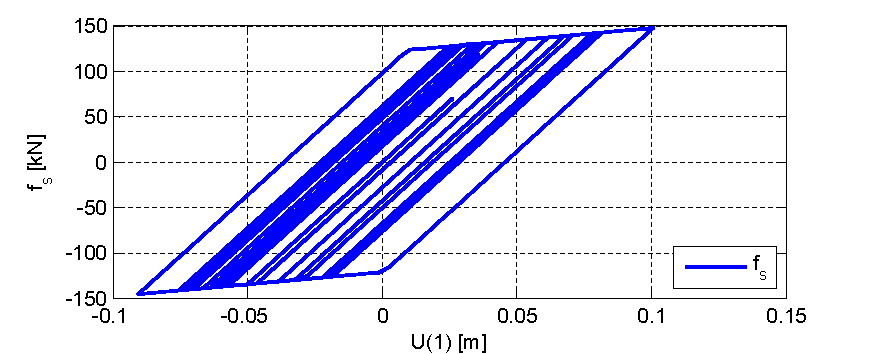
\includegraphics[ width=\textwidth]{83_hiszter.pdf}
\caption{A szeizmikus szigetelő elem  hiszterézis viselkedése a hibrid program számításai alapján.}
\label{fig:hiszt}
\end{figure}

  
A hibrid szimulációs programmal számított képlékeny anyagú szeizmikus szigeteléssel ellátott szerkezet abszolút, relatív és tetőponti elmozdulásait mutatja a \ref{fig:8_hibrid} ábra.





\subsection{Az eredmények összehasonlítása}

{\ }

A következőkben a fix megtámasztású szerkezet, a lineárisan rugalmas és a képlékeny szeizmikus szigeteléssel ellátott szerkezet számítási eredményeit hasonlítjuk össze az abszolút, a relatív és a tetőponti elmozdulások, valamint a keletkező  nyíróerők szerint. Ezeknek az egyes számításokból származó maximális értékeit a \ref{8_table} táblázat foglalja össze.

Az eredményekből kitűnik, hogy a szeizmikusan szigetelt épületek maximális abszolút elmozdulásai képlékeny esetben 5-ször, lineárisan rugalmas esetben több, mint 8-szor nagyobbak, mint a fix megtámasztású szerkezetnél, azonban a relatív elmozdulások esetében ez az arány fordított. A merev megtámasztású épület maximális relatív elmozdulása több, mint négyszerese a képlékeny, és majdnem nyolcszorosa a lineárisan rugalmas szigetelésű szerkezetnél számított relatív elmozdulásoknak. Ebből az következik, hogy  a maximális nyíróerők is ugyanakkora arányban csökkennek szeizmikus szigetelés esetében. A tetőponti elmozdulások fix megtámasztásnál az első szint elmozdulásainak többszörösére adódnak, míg szeizmikus szigetelésnél minimális az eltérés a tetőpont és az első szint maximális elmozdulásai között.

Mindez azt mutatja, hogy szeizmikus szigetelés esetében az épület inkább merevtest-szerűen eltolódik, a nagy deformációkat a szigetelés veszi fel, így a szerkezetben sokkal kisebb igénybevételek keletkeznek. 

\begin{figure}[!ht]%
\centering
\subfigure[][]{%
\label{fig:8_linfix-a}%
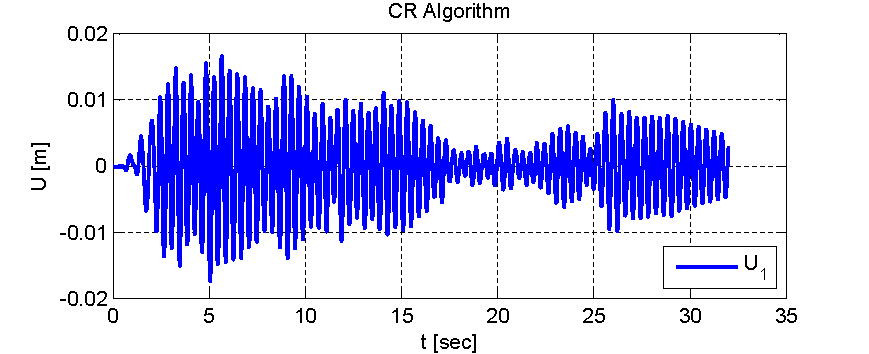
\includegraphics[width=0.9\textwidth]{81_u2.pdf}}%
\\
\subfigure[][]{%
\label{fig:8_linfix-b}%
\includegraphics[width=0.9\textwidth]{81_u5.pdf}}%
\caption[A lineáris programban vizsgált merev alapú  szerkezet elmozdulásai.]{A lineáris programban vizsgált merev alapú  szerkezet elmozdulásai:
\subref{fig:8_linfix-a} az első szint abszolút elmozdulásai; 
\subref{fig:8_linfix-b} tetőponti elmozdulások.}%
\label{fig:8_linfix}%
\end{figure}

\begin{figure}[!ht]%
\centering
\subfigure[][]{%
\label{fig:8_linbase-a}%
\includegraphics[width=0.9\textwidth]{82_u2.pdf}}%
\\
\subfigure[][]{%
\label{fig:8_linbase-b}%
\includegraphics[width=0.9\textwidth]{82_u_rel.pdf}}%
\\
\subfigure[][]{%
\label{fig:8_linbase-c}%
\includegraphics[width=0.9\textwidth]{82_u5.pdf}}%
\caption[A lineáris programban vizsgált szeizmikus szigeteléssel ellátott szerkezet elmozdulásai.]{A lineáris programban vizsgált szeizmikus szigeteléssel ellátott szerkezet elmozdulásai:
\subref{fig:8_linbase-a} az első szint abszolút elmozdulásai;
\subref{fig:8_linbase-b} az első szint relatív elmozdulásai; 
\subref{fig:8_linbase-c} tetőponti elmozdulások.}%
\label{fig:8_linbase}%
\end{figure}



\begin{figure}[!ht]%
\centering
\subfigure[][]{%
\label{fig:8_hibrid-a}%
\includegraphics[width=0.9\textwidth]{83_u2.pdf}}%
\\
\subfigure[][]{%
\label{fig:8_hibrid-b}%
\includegraphics[width=0.9\textwidth]{83_u_rel.pdf}}%
\\
\subfigure[][]{%
\label{fig:8_hibrid-c}%
\includegraphics[width=0.9\textwidth]{83_u5.pdf}}%
\caption[A hibrid programban vizsgált szeizmikus szigeteléssel ellátott szerkezet elmozdulásai.]{A hibrid programban vizsgált szeizmikus szigeteléssel ellátott szerkezet elmozdulásai:
\subref{fig:8_hibrid-a} az első szint abszolút elmozdulásai;
\subref{fig:8_hibrid-b} az első szint relatív elmozdulásai; 
\subref{fig:8_hibrid-c} tetőponti elmozdulások.}%
\label{fig:8_hibrid}%
\end{figure}



\begin{table}[h!]
\centering
\includegraphics[trim = 20mm 0mm 0mm 0mm, clip, width=\textwidth]{8_table.pdf}
\caption{A fix megtámasztású és a szeizmikus szigeteléssel ellátott épület maximális elmozdulásai és nyíróerői.}
\label{8_table}
\end{table}

Elmondható továbbá, hogy a szeizmikus szigetelés elsősorban a szigetelő rendszer  módjának sajátrezgésideje  miatt csökkenti a maximális nyíróerők értékét, mert a legtöbb válasz esetében ez sokkal hosszabb, mint a merev  épület sajátrezgésideje, és ez sokkal kisebb válaszspektrum ordinátához vezet.  A tervezési válaszspektrumot szilárd talajon, merev megtámasztású szerkezet esetében  a válaszspektrum  gyorsulásérzékeny területének lapos részében  a sajátperiódusidővel jellemezhetjük. A magasabb  módokat a földmozgás nem gerjeszti (még ha a pszeudo-gyorsulások nagyok is), mert a modális válaszok nagyon kicsik. 

Az eredményekből arra következtethetünk, hogy a szeizmikus szigetelés hatékonyan csökkenti a földrengés okozta erőket a szerkezetekben. Ennek elsődleges oka az  első mód periódusának meghosszabbodása. A szigetelő rendszer csillapító hatása és a járulékos energia disszipáció csak másodlagos tényező a strukturális válasz csökkentésében. 




\chapter{Összefoglalás}

{\ }

Dolgozatomban egy összefoglaló tanulmányban bemutattam a mozgásegyenletek megoldására alkalmazható időlépéses integrálás elméleti hátterét. Ismertettem a módszerek általános jellemzőit, majd a legfontosabb lineáris és nemlineáris integráló formulákat is. Összefoglaltam, hogy a különböző numerikus számításokat végző programok ezek közül mely integráló formulákat használják.

Az integráló algoritmusok  segítségével saját programokat fejlesztettem a lineáris és a nemlineáris dinamikus  feladatok megoldására, majd prezentáltam használatukat. A lineáris program használatát először egy gerjesztett rezgéses feladaton mutattam be, ahol a gerjesztés és a csillapítás hatását vizsgáltam, majd egy szabadrezgéses feladaton keresztül bemutattam, hogy a program hogyan használható az időlépéses módszerek stabilitásának és pontosságának vizsgálatára. A nemlineáris programnál először azt mutattam meg, hogy a program hogyan használható statikus  probléma vizsgálatára.  A feladatban az adott szerkezetet különböző csillapítási   tényezők  mellett alkalmaztam. Ezek után ismertettem a program használatát dinamikus probléma megoldására is. Szemléltettem a nemlinearitás hatását, valamint vizsgáltam a teherfüggvény módosításának hatását a rendszer elmozdulásaira.

Elvégeztem a lineáris és a nemlineáris programok verifikálását   Chopra  könyvében \cite{chopra} ismertetett szakirodalmi példákkal. A verifikáció mindkét esetben sikeres volt. A lineáris programban ugyanazok az eredmények születtek, mint a könyvben. A nemlineáris program esetében az eredmények között eltérések adódtak, de ezek egyértelműen betudhatók a feladatban alkalmazott anyagmodell hiányos ismertetésének.

Ezek után egy összefoglaló tanulmányban bemutattam a szerkezetek két különálló részre osztott, de összekapcsolt vizsgálatán alapuló  hibrid szimulációs eljárást. Összehasonlítottam más kísérleti eljárásokkal, bemutattam a módszer előnyeit, és a hozzá kapcsolódó főbb kihívásokat. Részleteztem az eljárás  lépéseit, és a szimuláció kivitelezésének különböző módjait.

A Chen-Ricles algoritmus alapján  hibrid programot fejlesztettem. Bemutattam a program használatát egy kétszintes,  nemlineáris merevítéssel ellátott szerkezeten. A szerkezeten az El Centro földrengésterhet működtettem. Elvégeztem a vizsgálatot, majd verifikáltam az eredményeket ugyanennek a szerkezetnek a nemlineáris megoldó programban végzett számításai alapján.

Végül alkalmaztam a hibrid szimulációs eljárást a szeizmikus szigetelések hatásának bemutatására. Az épület viselkedését összehasonlítottam egy a lineáris megoldó programban számított fix megtámasztású szerkezet, valamint egy a szintén a lineáris megoldóval számított szeizmikus szigeteléssel ellátott szerkezet viselkedésével. A hibrid programban vizsgált szerkezetre egy képlékeny anyagmodellt alkalmaztam. Láthattuk, hogy a szeizmikus szigetelés hatása jelentősen csökkenti az épületekben keletkező igénybevételeket.

Diplomamunkámban, a kiírt célkitűzéseknek megfelelően, vizsgálataimban bemutattam a mozgásegyenletek numerikus számításainak lehetőségeit, továbbá ismertettem a hibrid szimuláció elméleti hátterét, részleteztem az előnyeit, programommal pedig demonstráltam az alkalmazhatóságát. A földrengésre való tervezés előtérbe kerülése miatt szükség van új szerkezetek fejlesztésére, és azok viselkedésének vizsgálatára. Erre jelenleg a hibrid szimulációs eljárás a legalkalmasabb. A fentiek alapján elmondhatjuk, hogy az eljárást érdemes  hazánkban is megvalósítani, mert nagy előrelépést jelenthet a szeizmológiai védekezés  magyarországi kutatásaiban. 

\appendix

% \renewcommand{\chaptermark}[1]{%
% \markboth{\thechapter.%
% \ \chaptername.\ #1}{}}

\chapter{A lineáris megoldó program kódja}\label{chap: függ linprog}


 \lstinputlisting{"MATLAB/linear_system/main.m"}
 \lstinputlisting{"MATLAB/linear_system/init_system.m"}
  \lstinputlisting{"MATLAB/linear_system/integration_parameters.m"}
  \lstinputlisting{"MATLAB/linear_system/init_conditions.m"}
 \lstinputlisting{"MATLAB/linear_system/timestep.m"}
 

\chapter{A nemlineáris megoldó program kódja}\label{chap: függ nemlinprog}

\lstinputlisting{"MATLAB/nonlinear_system/main.m"}
 \lstinputlisting{"MATLAB/nonlinear_system/init_system.m"}
 \lstinputlisting{"MATLAB/nonlinear_system/integration_parameters.m"}
 \lstinputlisting{"MATLAB/nonlinear_system/init_conditions.m"}
 \lstinputlisting{"MATLAB/nonlinear_system/timestep.m"}
 \lstinputlisting{"MATLAB/nonlinear_system/resisting_force.m"}
 \lstinputlisting{"MATLAB/nonlinear_system/tangent_stiffness.m"}

\chapter{A lineáris megoldó program eredményei}\label{chap: függ eredmények}

\section{A \ref{subsec:lingerj} gerjesztett rezgéses  feladat elmozdulásai}\label{sec:függ_lingerj}

\begin{figure}[H]
\centering
\includegraphics[width=\textwidth]{312_Euler.pdf}
\caption{A \ref{subsec:lingerj} gerjesztett rezgéses példa elmozdulásai Euler módszerrel.}
\label{fig:függlingerjeredm_euler}
\end{figure}
\begin{figure}[H]
\centering
\includegraphics[width=\textwidth]{312_RK.pdf}
\caption{A \ref{subsec:lingerj} gerjesztett rezgéses példa elmozdulásai Runge-Kutta módszerrel.}
\label{fig:függlingerjeredm_rk}
\end{figure}
\begin{figure}[H]
\centering
\includegraphics[width=\textwidth]{312_cendiff.pdf}
\caption{A \ref{subsec:lingerj} gerjesztett rezgéses példa elmozdulásai centrális differenciák módszerével.}
\label{fig:függlingerjeredm_centdiff}
\end{figure}

\begin{figure}[H]
\centering
\includegraphics[width=\textwidth]{312_Newmark.pdf}
\caption{A \ref{subsec:lingerj} gerjesztett rezgéses példa elmozdulásai Newmark módszerrel.}
\label{fig:függlingerjeredm_newmark}
\end{figure}
\begin{figure}[H]
\centering
\includegraphics[width=\textwidth]{312_Wilson.pdf}
\caption{A \ref{subsec:lingerj} gerjesztett rezgéses példa elmozdulásai Wilson-$\boldsymbol\theta$ eljárással.}
\label{fig:függlingerjeredm_wilson}
\end{figure}
\begin{figure}[H]
\centering
\includegraphics[width=\textwidth]{312_HHT.pdf}
\caption{A \ref{subsec:lingerj} gerjesztett rezgéses példa elmozdulásai HHT-$\alpha$ módszerrel.}
\label{fig:függlingerjeredm_hht}
\end{figure}
\begin{figure}[H]
\centering
\includegraphics[width=\textwidth]{312_CR.pdf}
\caption{A \ref{subsec:lingerj} gerjesztett rezgéses példa elmozdulásai CR algoritmussal.}
\label{fig:függlingerjeredm_cr}
\end{figure}

\begin{figure}[H]
\centering
\includegraphics[width=\textwidth]{312_Newmark_Ku.pdf}
\caption{A \ref{subsec:lingerj} gerjesztett rezgéses példa elmozdulásai Newmark módszerrel és a statikus elmozdulás.}
\label{fig:függlingerjeredm_newmark_Ku}
\end{figure}


\section{A \ref{subsec:szabrezg} szabadrezgéses feladat eredményei}\label{sec:függ_szabrezg}

\subsection{A \ref{subsec:szabrezg} szabadrezgéses feladat elmozdulásai}\label{sec:függ_szabrezg_elm}

\begin{figure}[H]
\centering
\includegraphics[width=\textwidth]{313_Euler.pdf}
\caption{A \ref{subsec:szabrezg} szabadrezgéses példa elmozdulásai Euler módszerrel.}
\label{fig:függszabrezg_er_euler}
\end{figure}

\begin{figure}[H]
\centering
\includegraphics[width=\textwidth]{313_RK.pdf}
\caption{A \ref{subsec:szabrezg} szabadrezgéses példa elmozdulásai Runge-Kutta módszerrel.}
\label{fig:függszabrezg_er_rk}
\end{figure}

\begin{figure}[H]
\centering
\includegraphics[width=\textwidth]{313_cendiff.pdf}
\caption{A \ref{subsec:szabrezg} szabadrezgéses példa elmozdulásai centrális differenciák módszerével.}
\label{fig:függszabrezg_er_centdiff}
\end{figure}

\begin{figure}[H]
\centering
\includegraphics[width=\textwidth]{313_Newmark.pdf}
\caption{A \ref{subsec:szabrezg} gerjesztett rezgéses példa elmozdulásai Newmark módszerrel.}
\label{fig:függszabrezg_er_newmark}
\end{figure}

\begin{figure}[H]
\centering
\includegraphics[width=\textwidth]{313_Wilson.pdf}
\caption{A \ref{subsec:szabrezg} szabadrezgéses példa elmozdulásai Wilson-$\boldsymbol\theta$ eljárással.}
\label{fig:függszabrezg_er_wilson}
\end{figure}

\begin{figure}[H]
\centering
\includegraphics[width=\textwidth]{313_HHT.pdf}
\caption{A \ref{subsec:szabrezg} szabadrezgéses példa elmozdulásai HHT-$\alpha$ módszerrel.}
\label{fig:függszabrezg_er_hht}
\end{figure}

\begin{figure}[H]
\centering
\includegraphics[width=\textwidth]{313_CR.pdf}
\caption{A \ref{subsec:szabrezg} szabadrezgéses példa elmozdulásai CR algoritmussal.}
\label{fig:függszabrezg_er_cr}
\end{figure}

\subsection{A \ref{subsec:szabrezg} szabadrezgéses feladat mechanikai energiái}\label{sec:függ_szabrezg_mechen}

\begin{figure}[H]
\centering
\includegraphics[width=\textwidth]{313_Euler_mechen.pdf}
\caption{A \ref{subsec:szabrezg} szabadrezgéses példa mechanikai energiája Euler módszerrel.}
% \label{fig:függszabrezg_er_mechen_euler}
\end{figure}

\begin{figure}[H]
\centering
\includegraphics[width=\textwidth]{313_RK_mechen.pdf}
\caption{A \ref{subsec:szabrezg} szabadrezgéses példa mechanikai energiája Runge-Kutta módszerrel.}
% \label{fig:függszabrezg_er_mechen_rk}
\end{figure}

\begin{figure}[H]
\centering
\includegraphics[width=\textwidth]{313_cendiff_mechen.pdf}
\caption{A \ref{subsec:szabrezg} szabadrezgéses példa mechanikai energiája centrális differenciák módszerével.}
% \label{fig:függszabrezg_er_mechen_centdiff}
\end{figure}

\begin{figure}[H]
\centering
\includegraphics[width=\textwidth]{313_Newmark_mechen.pdf}
\caption{A \ref{subsec:szabrezg} szabadrezgéses példa mechanikai energiája Newmark módszerrel.}
% \label{fig:függszabrezg_er_mechen_newmark}
\end{figure}

\begin{figure}[H]
\centering
\includegraphics[width=\textwidth]{313_Wilson_mechen.pdf}
\caption{A \ref{subsec:szabrezg} szabadrezgéses példa mechanikai energiája Wilson-$\boldsymbol\theta$ eljárással.}
% \label{fig:függszabrezg_er_mechen_wilson}
\end{figure}

\begin{figure}[H]
\centering
\includegraphics[width=\textwidth]{313_HHT_mechen.pdf}
\caption{A \ref{subsec:szabrezg} szabadrezgéses példa mechanikai energiája HHT-$\alpha$ módszerrel.}
% \label{fig:függszabrezg_er_mechen_hht}
\end{figure}

\begin{figure}[H]
\centering
\includegraphics[width=\textwidth]{313_CR_mechen.pdf}
\caption{A \ref{subsec:szabrezg} szabadrezgéses példa mechanikai energiája CR algoritmussal.}
% \label{fig:függszabrezg_er_mechen_cr}
\end{figure}

\subsection{A \ref{subsec:szabrezg} szabadrezgéses feladat elmozdulásai fázistérben ábrázolva}\label{sec:függ_szabrezg_fázis}


\begin{figure}[H]
\centering
\includegraphics[width=\textwidth]{313_Euler_elm.pdf}
\caption{A \ref{subsec:szabrezg} szabadrezgéses példa elmozdulásai Euler módszerrel, fázistérben ábrázolva.}
% \label{fig:függszabrezg_er_elm_euler}
\end{figure}

\begin{figure}[H]
\centering
\includegraphics[width=\textwidth]{313_RK_elm.pdf}
\caption{A \ref{subsec:szabrezg} szabadrezgéses példa elmozdulásai Runge-Kutta módszerrel, fázistérben ábrázolva.}
% \label{fig:függszabrezg_er_elm_rk}
\end{figure}

\begin{figure}[H]
\centering
\includegraphics[width=\textwidth]{313_cendiff_elm.pdf}
\caption{A \ref{subsec:szabrezg} szabadrezgéses példa elmozdulásai centrális differenciák módszerével, fázistérben ábrázolva.}
% \label{fig:függszabrezg_er_elm_centdiff}
\end{figure}

\begin{figure}[H]
\centering
\includegraphics[width=\textwidth]{313_Newmark_elm.pdf}
\caption{A \ref{subsec:szabrezg} szabadrezgéses példa megoldása fázistérben ábrázolva Newmark módszerrel.}
% \label{fig:függszabrezg_er_elm_newmark}
\end{figure}

\begin{figure}[H]
\centering
\includegraphics[width=\textwidth]{313_Wilson_elm.pdf}
\caption{A \ref{subsec:szabrezg} szabadrezgéses példa elmozdulásai Wilson-$\boldsymbol\theta$ eljárással, fázistérben ábrázolva.}
K\label{fig:függszabrezg_er_elm_wilson}
\end{figure}

\begin{figure}[H]
\centering
\includegraphics[width=\textwidth]{313_HHT_elm.pdf}
\caption{A \ref{subsec:szabrezg} szabadrezgéses példa elmozdulásai HHT-$\alpha$ módszerrel, fázistérben ábrázolva.}
% \label{fig:függszabrezg_er_elm_hht}
\end{figure}

\begin{figure}[H]
\centering
\includegraphics[width=\textwidth]{313_CR_elm.pdf}
\caption{A \ref{subsec:szabrezg} szabadrezgéses példa elmozdulásai CR algoritmussal, fázistérben ábrázolva.}
% \label{fig:függszabrezg_er_elm_cr}
\end{figure}

\section{A nemlineáris megoldó program eredményei}

\subsection{A \ref{subsec:nemlinstat} statikus vizsgálat eredményei}\label{sec:függ 322}


\begin{figure}[H]
\centering
\includegraphics[width=\textwidth]{322_centdiff_kszi_0_1.pdf}
\caption{A \ref{subsec:nemlinstat} statikus probléma elmozdulásai centrális differenciák módszerével, $\xi = 0.1$-re.}
\label{fig:függ322_centdiff_0_1}
\end{figure}

\begin{figure}[H]
\centering
\includegraphics[width=\textwidth]{322_newmark_acc_kszi_0_1.pdf}
\caption{A \ref{subsec:nemlinstat} statikus probléma elmozdulásai a Newmark módszer gyorsulásos változatával, $\xi = 0.1$-re.}
\label{fig:függ322_newmark_acc_0_1}
\end{figure}

\begin{figure}[H]
\centering
\includegraphics[width=\textwidth]{322_newmark_disp_kszi_0_1.pdf}
\caption{A \ref{subsec:nemlinstat} statikus probléma elmozdulásai a Newmark módszer elmozdulásos változatával, $\xi = 0.1$-re.}
\label{fig:függ322_newmark_disp_0_1}
\end{figure}

\begin{figure}[H]
\centering
\includegraphics[width=\textwidth]{322_centdiff_kszi_0_5.pdf}
\caption{A \ref{subsec:nemlinstat} statikus probléma elmozdulásai centrális differenciák módszerével, $\xi = 0.5$-re.}
\label{fig:függ322_centdiff_0_5}
\end{figure}

\begin{figure}[H]
\centering
\includegraphics[width=\textwidth]{322_newmark_acc_kszi_0_5.pdf}
\caption{A \ref{subsec:nemlinstat} statikus probléma elmozdulásai a Newmark módszer gyorsulásos változatával, $\xi = 0.5$-re.}
\label{fig:függ322_newmark_acc_0_5}
\end{figure}

\begin{figure}[H]
\centering
\includegraphics[width=\textwidth]{322_newmark_disp_kszi_0_5.pdf}
\caption{A \ref{subsec:nemlinstat} statikus probléma elmozdulásai a Newmark módszer elmozdulásos változatával, $\xi = 0.5$-re.}
\label{fig:függ322_newmark_disp_0_5}
\end{figure}

\begin{figure}[H]
\centering
\includegraphics[width=\textwidth]{322_centdiff_kszi_1_1.pdf}
\caption{A \ref{subsec:nemlinstat} statikus probléma elmozdulásai centrális differenciák módszerével, $\xi = 1.1$-re.}
\label{fig:függ322_centdiff_1_1}
\end{figure}

\begin{figure}[H]
\centering
\includegraphics[width=\textwidth]{322_newmark_acc_kszi_1_1.pdf}
\caption{A \ref{subsec:nemlinstat} statikus probléma elmozdulásai a Newmark módszer gyorsulásos változatával, $\xi = 1.1$-re.}
\label{fig:függ322_newmark_acc_1_1}
\end{figure}

\begin{figure}[H]
\centering
\includegraphics[width=\textwidth]{322_newmark_disp_kszi_1_1.pdf}
\caption{A \ref{subsec:nemlinstat} statikus probléma elmozdulásai a Newmark módszer elmozdulásos változatával, $\xi = 1.1$-re.}
\label{fig:függ322_newmark_disp_1_1}
\end{figure}


\subsection{A \ref{subsec:nemlindin} dinamikus vizsgálat eredményei}\label{sec:függ 323}


\begin{figure}[H]
\centering
\includegraphics[width=\textwidth]{323_centdiff.pdf}
\caption{A \ref{subsec:nemlindin} dinamikus probléma elmozdulásai centrális differenciák módszerével.}
\label{fig:függ323_centdiff}
\end{figure}

\begin{figure}[H]
\centering
\includegraphics[width=\textwidth]{323_Newmark_acc.pdf}
\caption{A \ref{subsec:nemlindin} dinamikus probléma elmozdulásai a Newmark módszer gyorsulásos változatával.}
\label{fig:függ323_newmark_acc}
\end{figure}

\begin{figure}[H]
\centering
\includegraphics[width=\textwidth]{323_Newmark_disp.pdf}
\caption{A \ref{subsec:nemlindin} dinamikus probléma elmozdulásai a Newmark módszer elmozdulásos változatával.}
\label{fig:függ323_newmark_disp}
\end{figure}


\begin{figure}[H]
\centering
\includegraphics[width=\textwidth]{323_centdiff_q_var.pdf}
\caption{A \ref{subsec:nemlindin} dinamikus probléma megoldásai az első csomópontra  centrális differenciák módszerével különböző terhelésekre.}
\label{fig:függ323_newmark_disp_q_var_1}
\end{figure}

\begin{figure}[H]
\centering
\includegraphics[width=\textwidth]{323_Newmark_acc_q_var.pdf}
\caption{A \ref{subsec:nemlindin} dinamikus probléma megoldásai az első csomópontra a Newmark módszer gyorsulásos változatával különböző terhelésekre.}
\label{fig:függ323_newmark_disp_q_var_1}
\end{figure}

\begin{figure}[H]
\centering
\includegraphics[width=\textwidth]{323_Newmark_disp_q_var.pdf}
\caption{A \ref{subsec:nemlindin} dinamikus probléma megoldásai az első csomópontra a Newmark módszer elmozdulásos változatával különböző terhelésekre.}
\label{fig:függ323_newmark_disp_q_var_1}
\end{figure}



\chapter{A hibrid szimulációs program kódja}\label{chap: függ hibrid prog}

\lstinputlisting{"MATLAB/hibrid/main.m"}
 \lstinputlisting{"MATLAB/hibrid_72/init_system.m"}
 \lstinputlisting{"MATLAB/hibrid/init_conditions.m"}

 \lstinputlisting{"MATLAB/hibrid/convert_num2lab.m"}
 \lstinputlisting{"MATLAB/hibrid/labor.m"}
 \lstinputlisting{"MATLAB/hibrid/convert_lab2num.m"}
 \lstinputlisting{"MATLAB/hibrid/timestep.m"}
 \lstinputlisting{"MATLAB/hibrid/resisting_force.m"}
 \lstinputlisting{"MATLAB/hibrid/U_num2lab.m"}
 \lstinputlisting{"MATLAB/hibrid/f_s_lab2num.m"}
 
 Az  földrengések adatait beolvasó függvény:
 \lstinputlisting{"MATLAB/hibrid_72/EQ_load.m"}

 

\begin{thebibliography}{1}
\thispagestyle{empty}

\bibitem{gyorgyi} Györgyi József: Szerkezetek dinamikája. Műegyetemi Kiadó, Budapest (2006).
  
\bibitem{chopra} Chopra, A. K.: Dynamics of Structures: Theory and Applications to Earthquake Engineering (4th edn).  Prentice-Hall, Upper Saddle River, New Jersey (2001).

% \bibitem{veges} Bojtár I., Gáspár Zs.: Végeselemmódszer építőmérnököknek. Terc Kft., Budapest (2003).

\bibitem{crcontthe} Chen C., Ricles JM.: Development of direct integration algorithms for structural dynamics using discrete control theory. Journal of Engineering Mechanics \textcopyright ASCE / August (2008).

\bibitem{crhybrid} Chen C., Ricles JM., Marullo TM., Mercan O.: Real-time hybrid testing using the unconditionalli stable explicit CR integration algorithm. Earthquake Engineering and Structural Dynamics, 38:23-44 (2009). 

\bibitem{molnar} Molnár Gergely, Bojtár Imre: 1D nemlineáris feladatok végeselemes vizsgálata explicit időintegrálással. Építés-Építészettudomány, 40 (1-2), 5-32  (2012).

\bibitem{hht} D. Negrut, R. Rampalli, G. Ottarsson, A. Sajdak: On the Use of the HHT Method in the Context of Index 3
Differential Algebraic Equations of Multibody Dynamics. Int. J. Numer. Meth. Engng., 00:1-6 , (2000).

\bibitem{hht_wiki}\url{ http://opensees.berkeley.edu/wiki/index.php/Hilber-Hughes-Taylor_Method}, (2014.03.11.).

\bibitem{nummat} Faragó István, Horváth Róbert: Numerikus módszerek.\url{tankonyvtar.ttk.bm.hu}, (2013).

\bibitem{hibrid} Andreas H. Schellenberg,  Stephen A. Mahin, Gregory L. Fenves: Advanced Implementation of Hybrid Simulation. PEER Report.Pacific Earthquake Engineering Research Center.  (2009).

\bibitem{hibrid wiki}\url{http://nees.org}, (2014.04.10.).

\bibitem{mónus} Tóth L, Mónus P, Zsíros T, Kiszely M: A Pannon-medence szeizmicitása. Földtani Közlöny 132/különszám, 327-337, (2002).

\bibitem{évkönyv} Tóth L., Mónus P., Kiszely M.: Magyarországi földrengések évkönyve 2013. GeoRisk, Budapest, HU ISSN: 1589-8326, (2014).

\bibitem{shaking}\url{http://www.seasva.gwu.edu/gwu/research_centers/lisr/Shake%20Table.html}, (2014.05.03.).

\bibitem{quasi}\url{http://www.ibk.ethz.ch/masonry/research/dcsm}(2014.05.03.).

\bibitem{elcentro}\url{http://www.vibrationdata.com/elcentro.dat}(2014.05.12.)

\bibitem{simon vigh} Simon József, Vigh L. Gergely: Hidak megerősítése szeizmikus hatásokkal szemben. Építményeink védelme 2013. Ráckeve, Magyarország (2013).

\bibitem{ec8} CEN: EN 1998-1:2008 Eurocode 8: Design of structures for earthquake resistance - Part 1: General rules, seismic actions and rules for buildings (2008).

\bibitem{antiizé}  CEN: EN 15129:2009 : Anti-seismic devices (2009).

\bibitem{rubber} Aykut Erkal, Semih S. Tezcan, Debra F. Laefer: Assessment and Code Considerations for the Combined Effect of Seismic Base Isolation and Viscoelastic Dampers. ISRN Civil Engineering, Article ID 861451 (2011).

\bibitem{lehigh} \url{http://www.nees.lehigh.edu/}(2014.05.20.)

 \thispagestyle{empty}
\end{thebibliography}

\end{document}
